% !TEX root = ../../Tesi_Triennale_PMNS.tex
\chapter{Analisi}
\label{chapter:analisi}
\begin{wrapfigure}{r}{0.4\textwidth}
	\vspace{-10pt}
	\begin{center}
		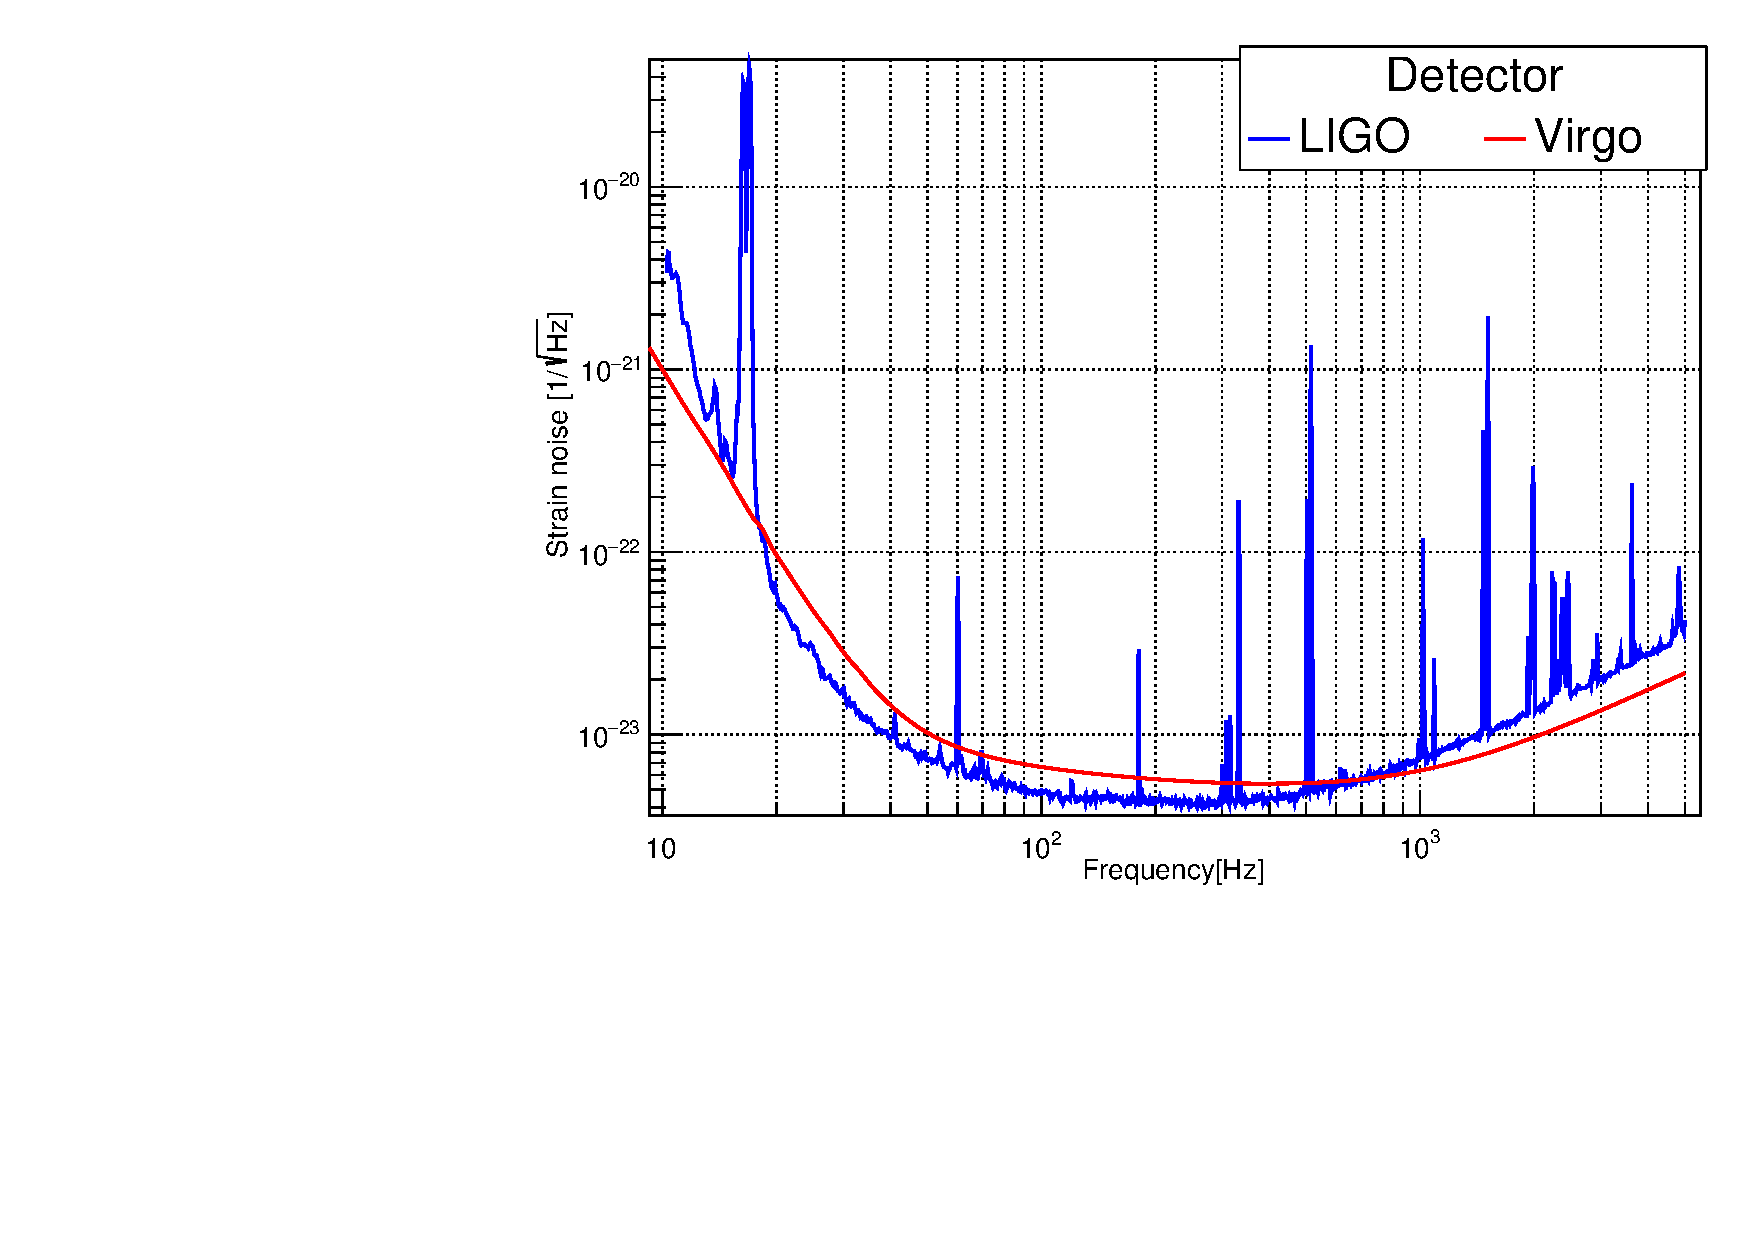
\includegraphics[width=0.4\textwidth]{figures/Capitolo_4/report/pds.pdf}
	\end{center}
	\vspace{-5pt}
	\caption{Sensibilità della rete}
	\label{fig:sensitivity_O4}
	\vspace{-10pt}
\end{wrapfigure}
Verrà presentata in questo capitolo un'analisi basata su un grande numero di forme d'onda iniettate in posizioni celesti generiche e ricostruite con cWB. Dopo aver mostrato preliminarmente un esempio di analisi di un evento singolo, verrà presentata l'analisi obiettivo di questa tesi: nella prima parte verrà fatta l'analisi delle curve di sensibilità e degli overlap, mentre la seconda parte sarà un'analisi volta a stimare sistematicamente la frequenza della post-coaelescenza, in particolare utilizzata sulle EOS APR4 e SHT2.
Le simulazioni utilizzano stime intermedie per le sensibilità che raggiungerà la rete LIGO-Virgo nel run O4 le cui sensibilità si possono osservare nel grafico delle PSD in Figura \ref{fig:sensitivity_O4}, non si considera invece il rivelatore Kagra, nonostante sia previsto il suo utilizzo ben prima.\\
Si osserva che per i rivelatori LIGO-Hanford e LIGO-Livingstone le curve risultano ben caratterizzate avendo, oltre alla curva teorica, foreste di picchi frutto di risonanze e altri fenomeni che ne compromettono in parte la sensibilità; per Virgo invece tale caratterizzazione non è stata fatta, motivo per il quale si lavorerà con una sensibilità generalmente sovrastimata rispetto ai risultati che si potranno ottenere nel run O4.\\
Si osserva inoltre che la curva per LIGO risulta più performante a frequenze intermedie, nella quale si presentano gli eventi di coalescenza di buchi neri e la parte dello spiraleggiamento per la coalescenza di stelle di neutroni; le due curve si scambiano invece ad alte frequenze, dove il rivelatore Virgo risulta più performante grazie alla tecnica dello squeezing che permette di guadagnare sensibilità ad alte frequenze.
\section{Esempi di analisi utilizzando cWB}
\label{section:examples}
Vengono ora riportati alcuni esempi di analisi di eventi simulati e ricostruiti utilizzando cWB, partendo da forme d'onda simulate a partire da due diverse EOS: APR4 e SHT2. Per quest'ultima in particolare viene presentata l'analisi per due condizioni iniziali: SHT2.0 e SHT2.2, che differiscono solo per le masse iniziali: la prima parte da masse delle stelle progenitrici tali da portare il sistema in ipermassiva, mentre la seconda ha il ringdown che porta il sistema in buco nero. Per la EOS APR4 la forma d'onda è in Figura \ref{fig:forma_onda_APR4} e non si riporterà di nuovo per ragioni di spazio, si riportano invece in Figura \ref{fig:forme_onda} le forme d'onda iniettate negli altri casi
\begin{figure}[ht]
	\vspace{-10pt}
	\centering
	\subfloat[][\emph{SHT2.0}]
	{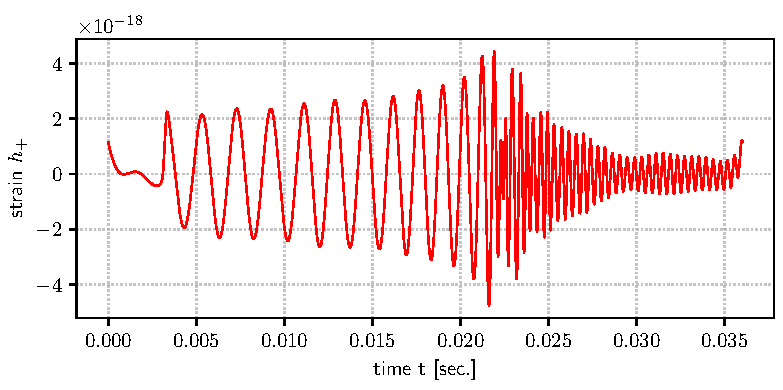
\includegraphics[width=.45\textwidth]{figures/Capitolo_4/SHT2.0.pdf}}\quad
	\subfloat[][\emph{SHT2.2}]
	{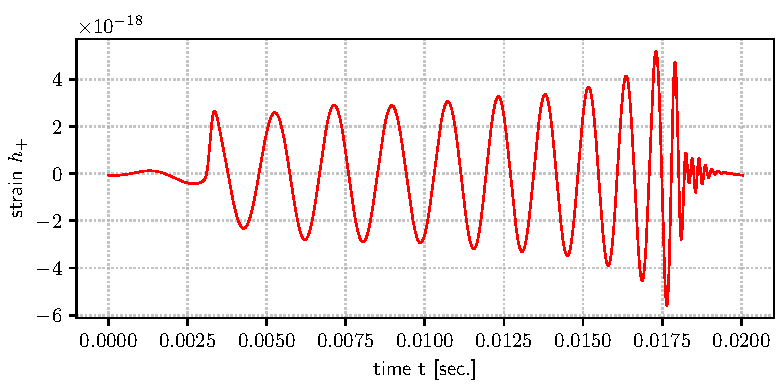
\includegraphics[width=.45\textwidth]{figures/Capitolo_4/SHT2.2.pdf}}
	\vspace{-5pt}
	\caption{Forme d'onda iniettate per l'equazione di stato SHT2, per le due configurazioni massive}
	\label{fig:forme_onda}
	\vspace{-15pt}
\end{figure}
\subsection{Equazione di stato APR4}
\label{subsection:APR4}
\begin{wraptable}{r}{0.4\textwidth}
	\vspace{-8pt}
	\begin{tabular}{cccccc}
		\toprule
		SNR	&$\rho$	&$c_{net}$	&ED	&$\theta$	&$\phi$	\\
		\midrule
		103.1	&50.8	&0.97	&-0.1	&101.6	&-28.6	\\
		\bottomrule
	\end{tabular}
	\vspace{-5pt}
\end{wraptable}
Si riportano i principali coefficienti per identificare l'evento: il rapporto segnale su rumore (SNR); il valore del coefficiente $\rho$, ovvero una ranking statistic che esprime la significanza del segnale descrivendo l'ampiezza correlata effettiva; il coefficiente $c_{net}$ descritto in equazione \ref{eqn:coefficient_energy}; ED che descrive lo sbilanciamento dell'energia tra i rivelatori nella rete e, infine, $\theta$ e $\phi$ che descrivono la posizione celeste della sorgente.
\begin{figure}[ht]
	\vspace{-10pt}
	\centering
	\subfloat[][\emph{LIGO-Livingstone}]
	{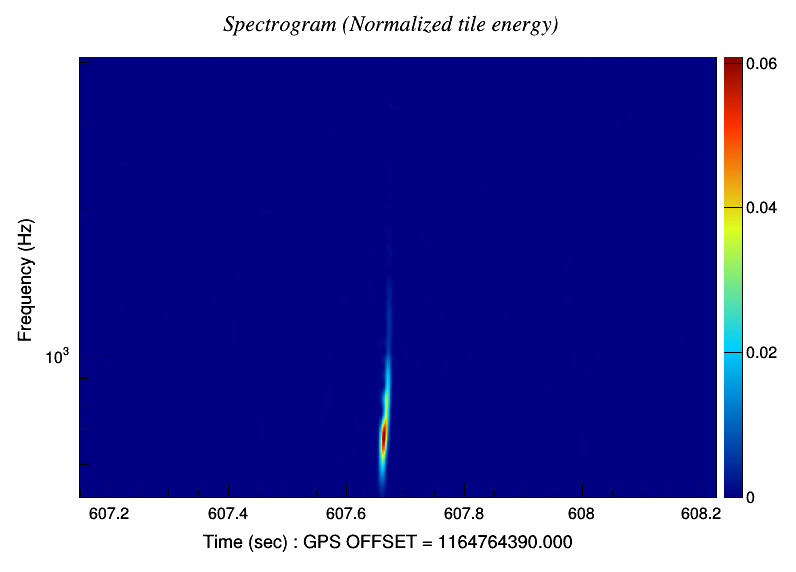
\includegraphics[width=.333333333\textwidth]{figures/Capitolo_4/APR4_q09/L1_spectrogram_logy_0.png}}
	\subfloat[][\emph{LIGO-Hanford}]
	{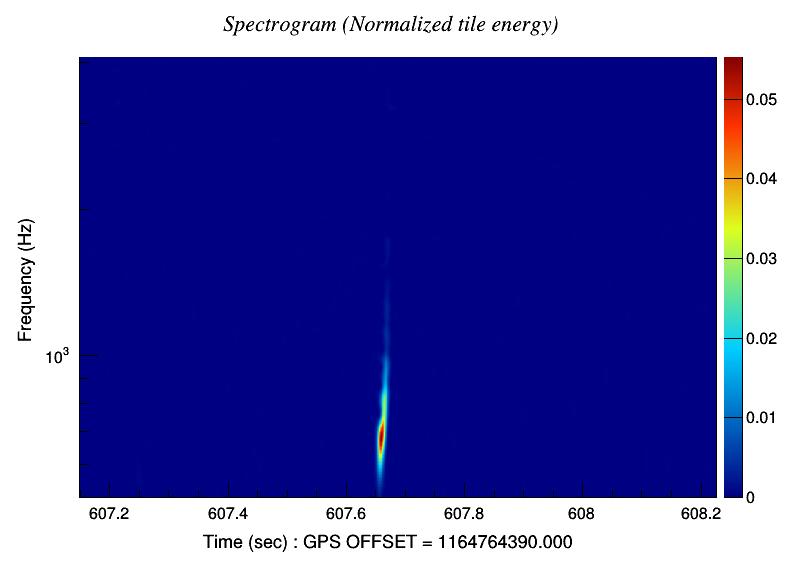
\includegraphics[width=.333333333\textwidth]{figures/Capitolo_4/APR4_q09/H1_spectrogram_logy_0.png}}
	\subfloat[][\emph{Virgo}]
	{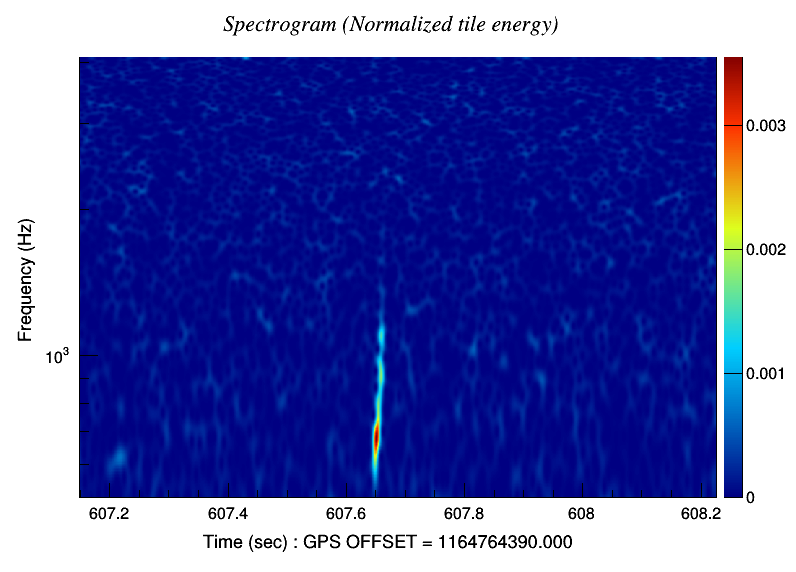
\includegraphics[width=.333333333\textwidth]{figures/Capitolo_4/APR4_q09/V1_spectrogram_logy_0.png}}
	\vspace{-5pt}
	\caption{Spettrogrammi per ciascun rivelatore, che mostrano una rappresentazione sul piano tempo-frequenza del trigger, basandosi sulla scomposizione di Fourier}
	\label{fig:spettrogramma_apr4}
	\vspace{-15pt}
\end{figure}

Il segnale che si mostra è particolarmente energetico, perché simulato a distanza ravvicinata ($d \simeq 1.25$Mpc). Si osservano quindi coefficienti particolarmente elevati.
Come si può osservare in Figura \ref{fig:spettrogramma_apr4}, mentre i rivelatori LIGO-Livingstone e LIGO-Handford rivelano in modo evidente un segnale già ad un'analisi visiva, senza eccessi di rumore significativi a sporcare la rivelazione, nella mappa di Virgo risulta distinguibile il segnale, tuttavia con rumore significativo e si può notare anche come guardando la scala di significanze del segnale questo risulti di un ordine di grandezza inferiore per Virgo, rispetto ai due rivelatori LIGO. 
\begin{wrapfigure}{r}{0.4\textwidth}
	\vspace{-15pt}
	\begin{center}
		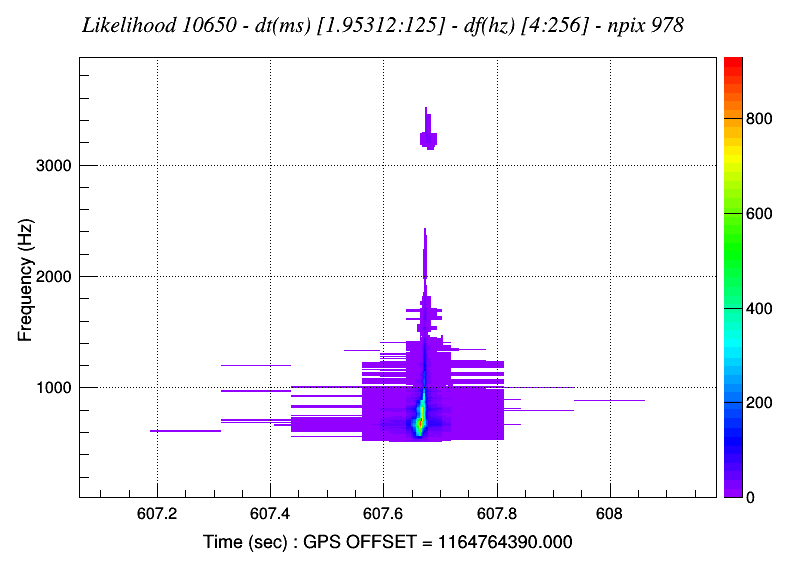
\includegraphics[width=0.4\textwidth]{figures/Capitolo_4/APR4_q09/l_tfmap_scalogram.png}
	\end{center}
	\vspace{-8pt}
	\caption{Mappa di verosimiglianza nel piano tempo-frequenza, che descrive il contributo dell'energia totale del campione associato all'evento ricostruito}
	\label{fig:Likelihood_APR4}
	\vspace{-15pt}
\end{wrapfigure}
Questo è probabilmente dovuto al fatto che i rivelatori LIGO sono allineati tra loro, mentre disallineati rispetto a Virgo e soprattutto alla posizione celeste della sorgente, favorevole ai primi due.\\
Nel grafico della likelihood in Figura \ref{fig:Likelihood_APR4}, si osserva un tipico andamento a chirp, in cui la parte inferiore, a basse frequenze, rappresenta lo spiraleggiamento fino alla coalescenza, mentre il cluster di dati in alto, a frequenze particolarmente elevate ($\smallsim 3.3$KHz) corrisponde all'emissione della post-coalescenza.
Infine nei grafici che seguono in Figura \ref{fig:strain_apr4} si osservano le ricostruzioni della forma d'onda, in particolare in nero è plottato il segnale iniettato nella simulazione, mentre in rosso il segnale ricostruito. In particolare osservando il grafico delle frequenze si può notare come non sia stato ricostruito tra $\smallsim$2.5KHz e $\smallsim3$KHz, giustificando la separazione tra i cluster nel grafico della likelihood.
\begin{figure}[H]
	\vspace{-25pt}
	\centering
	\subfloat[][\emph{Dominio dei tempi}]
	{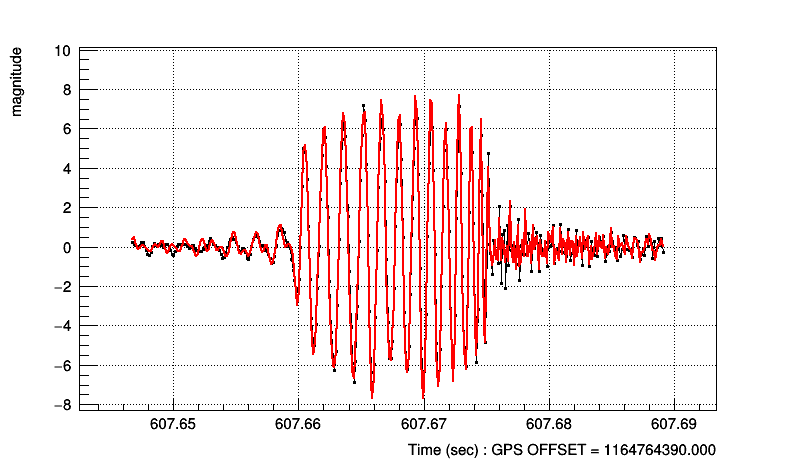
\includegraphics[width=.4\textwidth]{figures/Capitolo_4/APR4_q09/L1_wf_white_inj_rec.png}} \quad\quad
	\subfloat[][\emph{Dominio delle frequenze}]
	{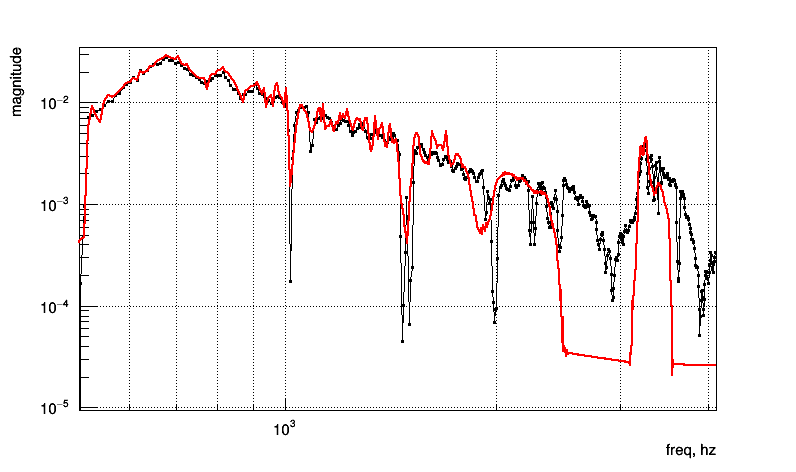
\includegraphics[width=.4\textwidth]{figures/Capitolo_4/APR4_q09/L1_wf_white_inj_rec_fft.png}}
	\vspace{-5pt}
	\caption{Ampiezza di strain ricostruita nel dominio dei tempi e nel dominio delle frequenze relative a un solo rivelatore}
	\label{fig:strain_apr4}
	\vspace{-15pt}
\end{figure}
\subsection{Equazione di stato SHT2}
\label{subsection:SHT2}
Per motivi di spazio non verranno presentate le analisi complete, come per l'equazione di stato precedente, ma si mostreranno solo i grafici delle likelihood: le due forme d'onda iniettate differiscono per la massa delle NS per la coalescenza, in particolare nella Figura \ref{fig:likelihood_sht2}(a), con masse tali da andare in ipermassiva, si può notare come sia presente un segnale di post-merger a $\smallsim 2.5$kHz mentre nella Figura \ref{fig:likelihood_sht2}(b), che ha masse tali da andare direttamente in buco nero, non vi è nessun segnale di post-merger ma solo un segnale di merger che arriva ad alte frequenze. 
\begin{figure}[H]
	\vspace{-20pt}
	\centering
	\subfloat[][\emph{SHT2.0}]
	{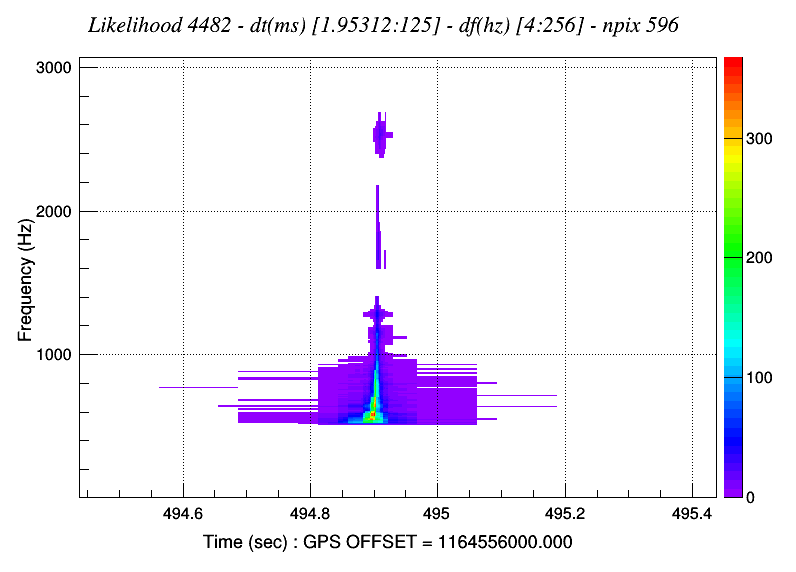
\includegraphics[width=.5\textwidth]{figures/Capitolo_4/SHT2.0spinf1_1/l_tfmap_scalogram.png}}
	\subfloat[][\emph{SHT2.2}]
	{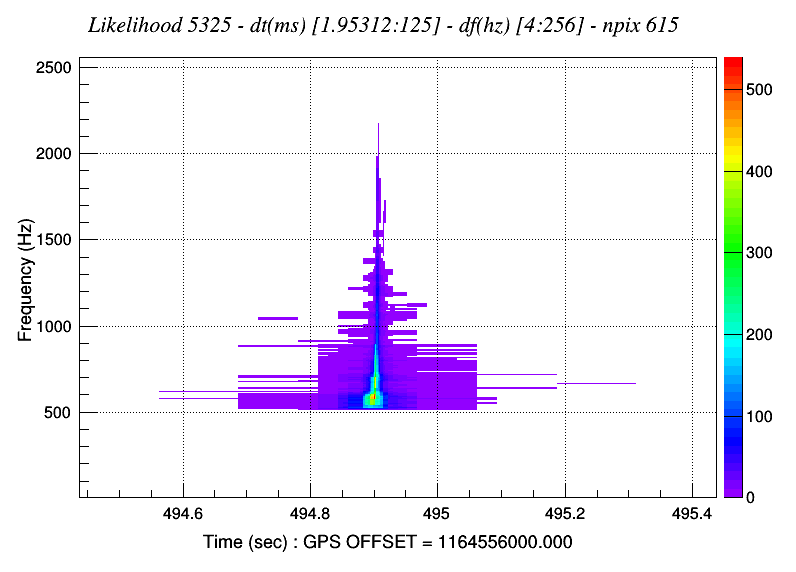
\includegraphics[width=.5\textwidth]{figures/Capitolo_4/SHT2.2spinf1_1/l_tfmap_scalogram.png}}
	\vspace{-5pt}
	\caption{Mappe di verosimiglianza ricostruite per le due forme d'onda iniettate}
	\label{fig:likelihood_sht2}
	\vspace{-15pt}
\end{figure}

\section{Curve di sensibilità e analisi dell'overlap}
\label{section:overlap}
\subsection{Caratteristiche degli eventi simulati}
\label{subsection:cwb_injections}
La post coalescenza, come già detto, è allo stato attuale difficile da rivelare a causa della scarsa sensibilità dei rivelatori a tali frequenze, per questo le analisi che vengono fatte in questa tesi non coivolgeranno dati misurati, ma dati simulati che vengono iniettati in rumore gaussiano, anch'esso simulato.\\
In particolare è stato simulato un considerevole numero di eventi ($\smallsim 5000$ eventi), che vengono poi ricostruiti con l'algoritmo cWB per verificarne la capacità di ricostruzione e studiare questi eventi.\\
Gli eventi simulati vengono prodotti a 5 diverse distanze [20, 10, 5, 2.5, 1.25]Mpc e distribuiti in modo uniforme nel cielo, in particolare i grafici di tali distribuzioni sono riportati in Figura \ref{fig:skypos}. Inoltre gli eventi vengono simulati in modo che anche le polarizzazioni siano distribuite uniformemente.
\begin{figure}[ht]
	\vspace{-20pt}
	\centering
	\subfloat[][\emph{Distribuzione distanze}]
	{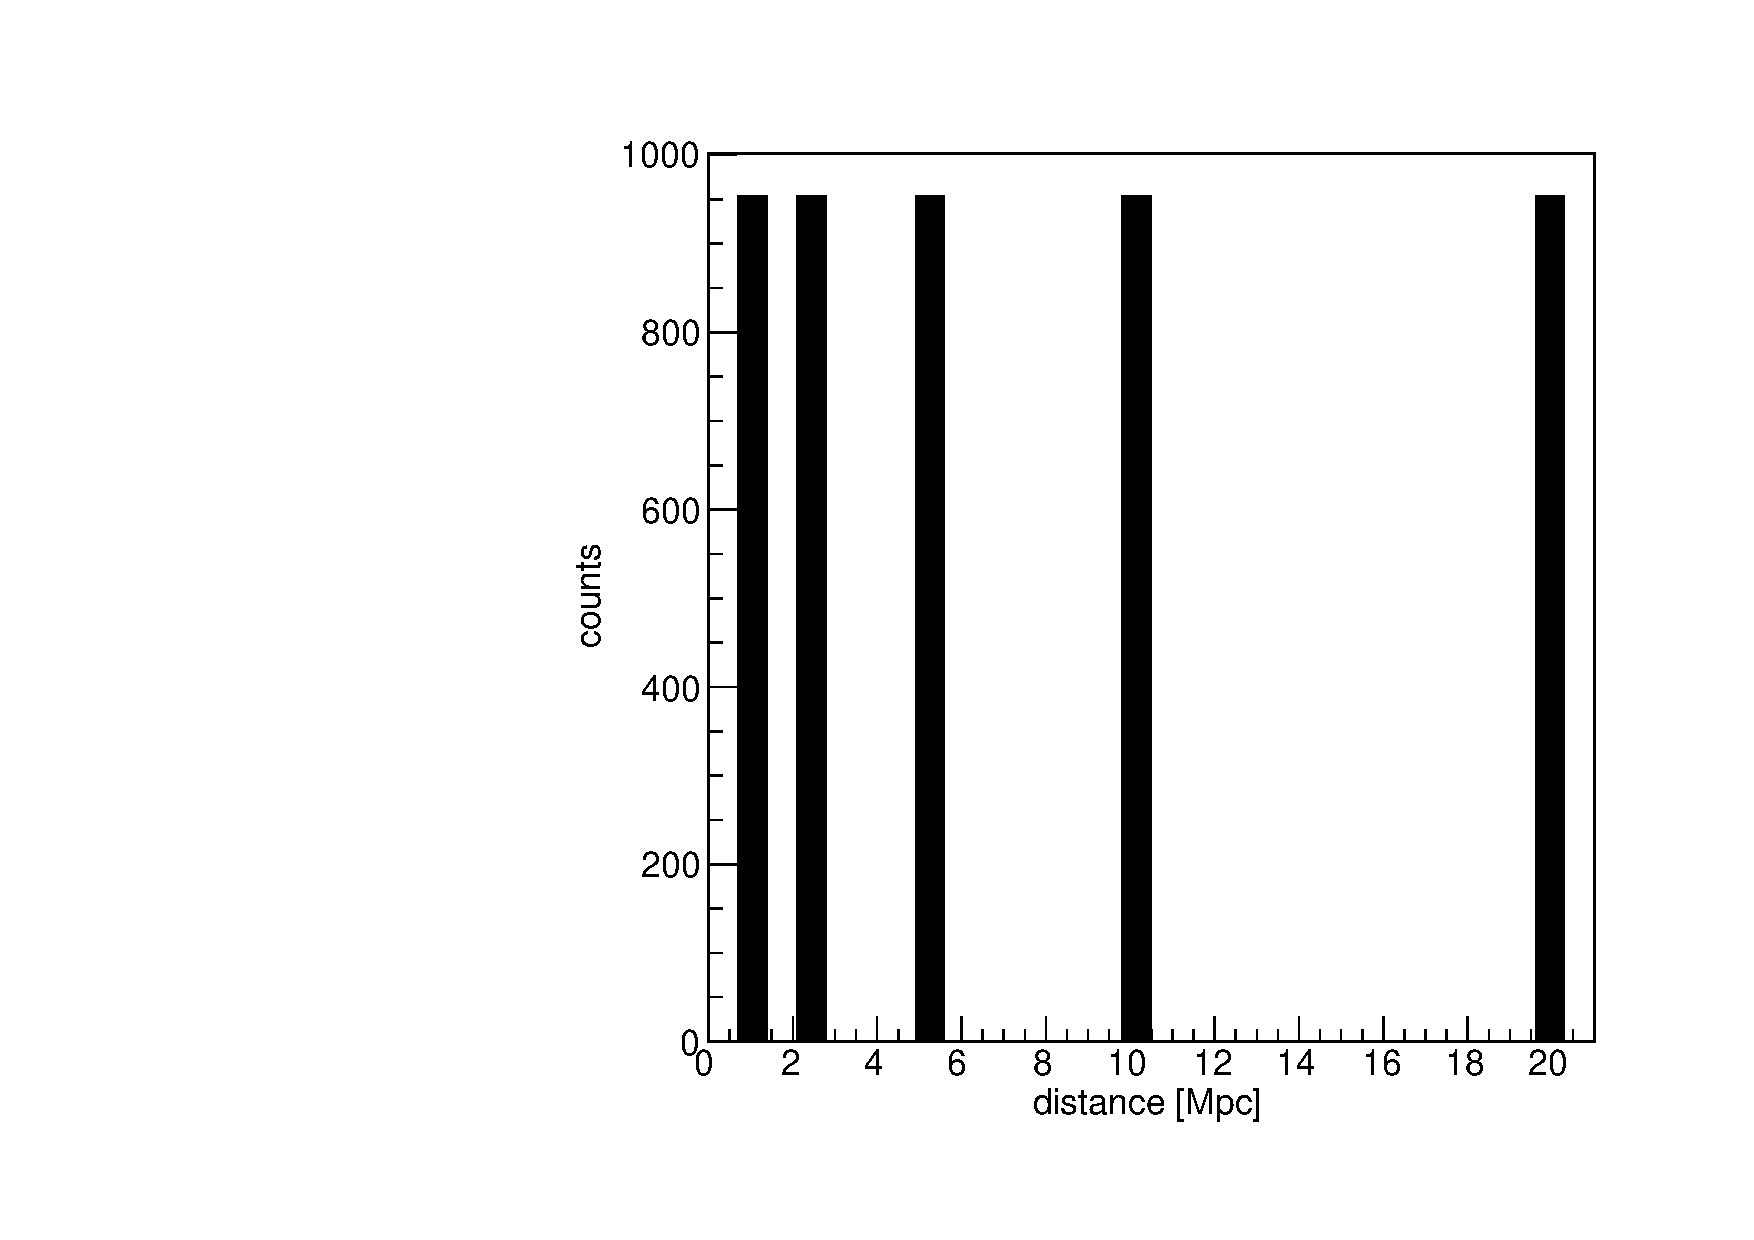
\includegraphics[width=.3\textwidth]{figures/Capitolo_4/report/factorsSHT2_0spin1.pdf}}\quad
	\subfloat[][\emph{Distribuzione celeste}]
	{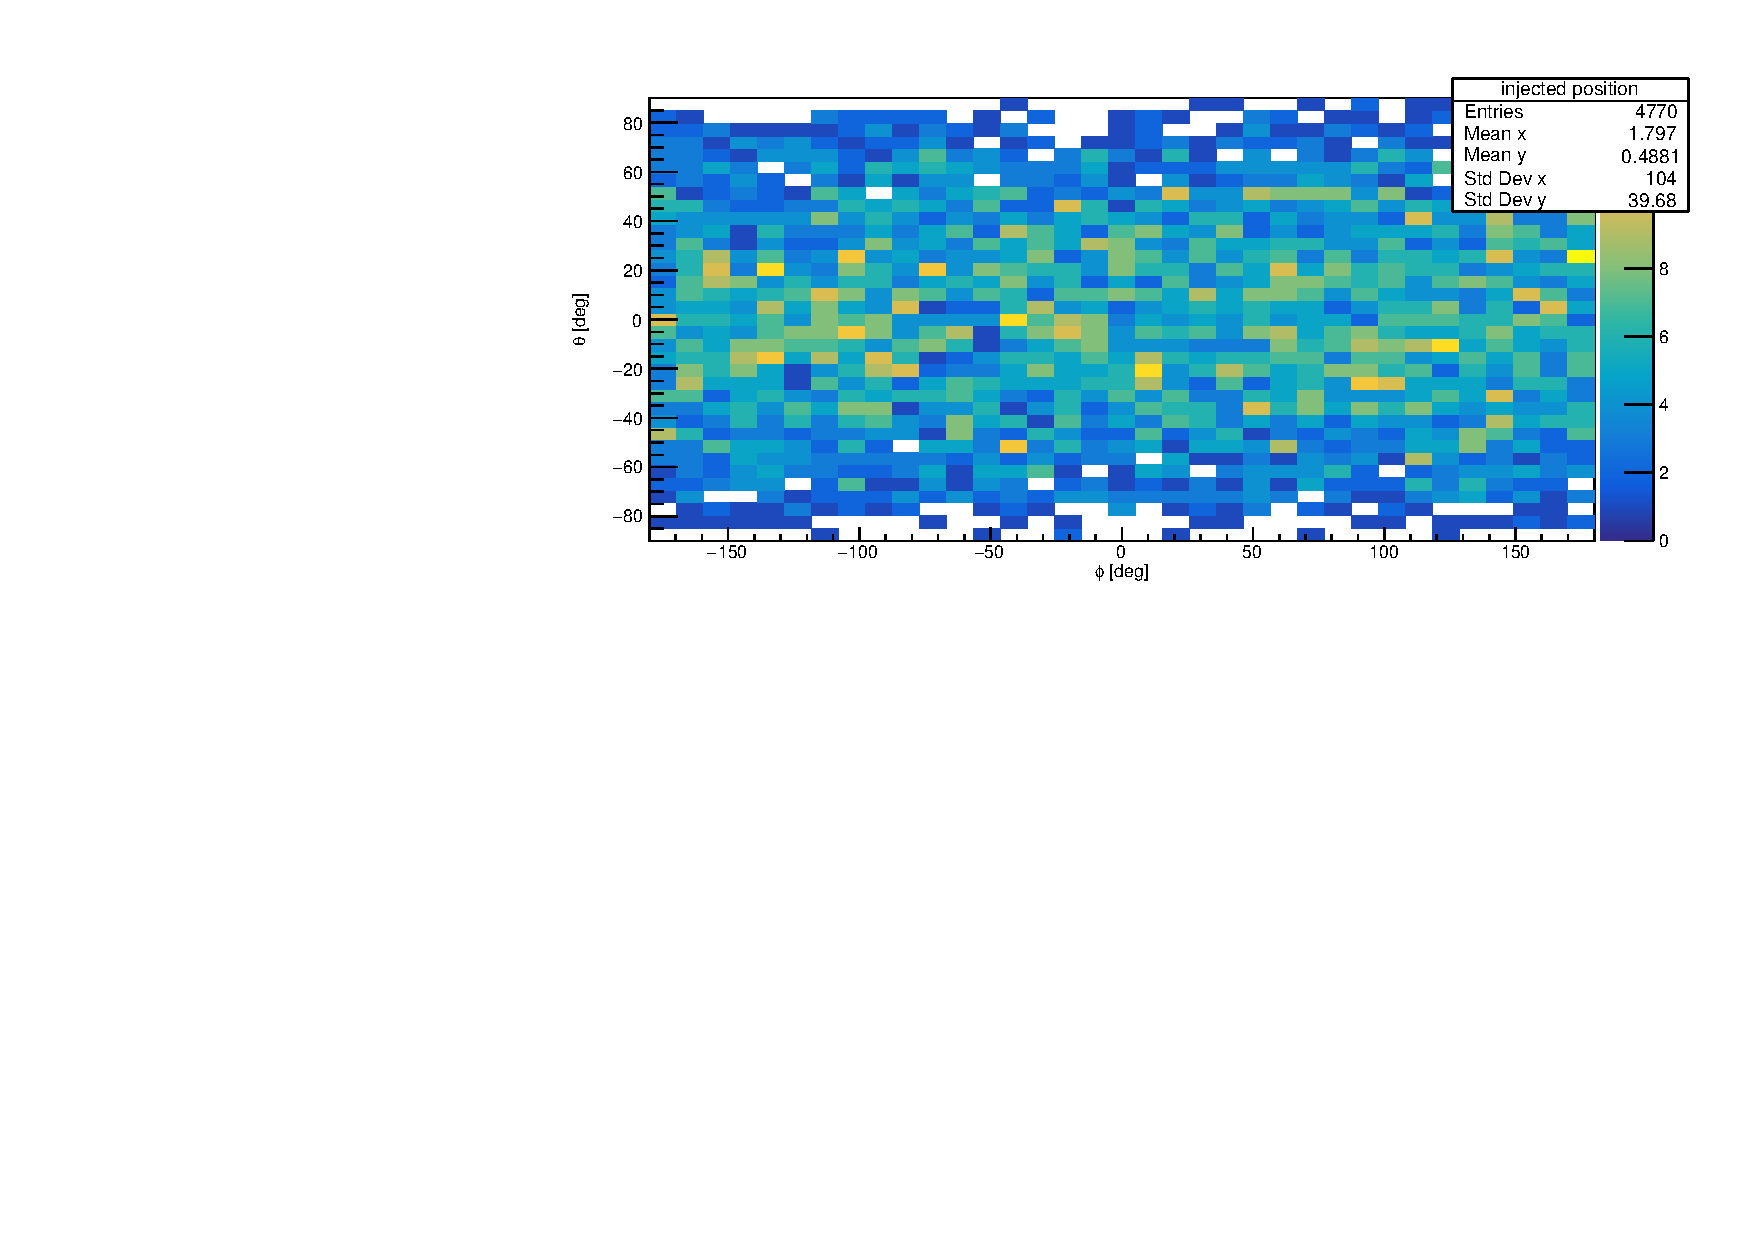
\includegraphics[width=.6\textwidth]{figures/Capitolo_4/report/ipositionSHT2_0spin1.pdf}}
	\vspace{-5pt}
	\caption{Distribuzione degli eventi simulati per l'EOS SHT2.0}
	\label{fig:skypos}
	\vspace{-10pt}
\end{figure}
Si riporta poi, in Figura \ref{fig:SNR_INJ_REC_COUNTS}, la distribuzione dei rapporti segnale su rumore, divisi per le distanze. Si nota immediatamente come al crescere della distanza gli eventi siano meno energetici, mentre per gli eventi molto vicini gli SNR arrivino a grandezze considerevoli. \\
\begin{figure}[ht]
	\vspace{-10pt}
	\centering
	\subfloat[][\emph{SHT2.0}]
	{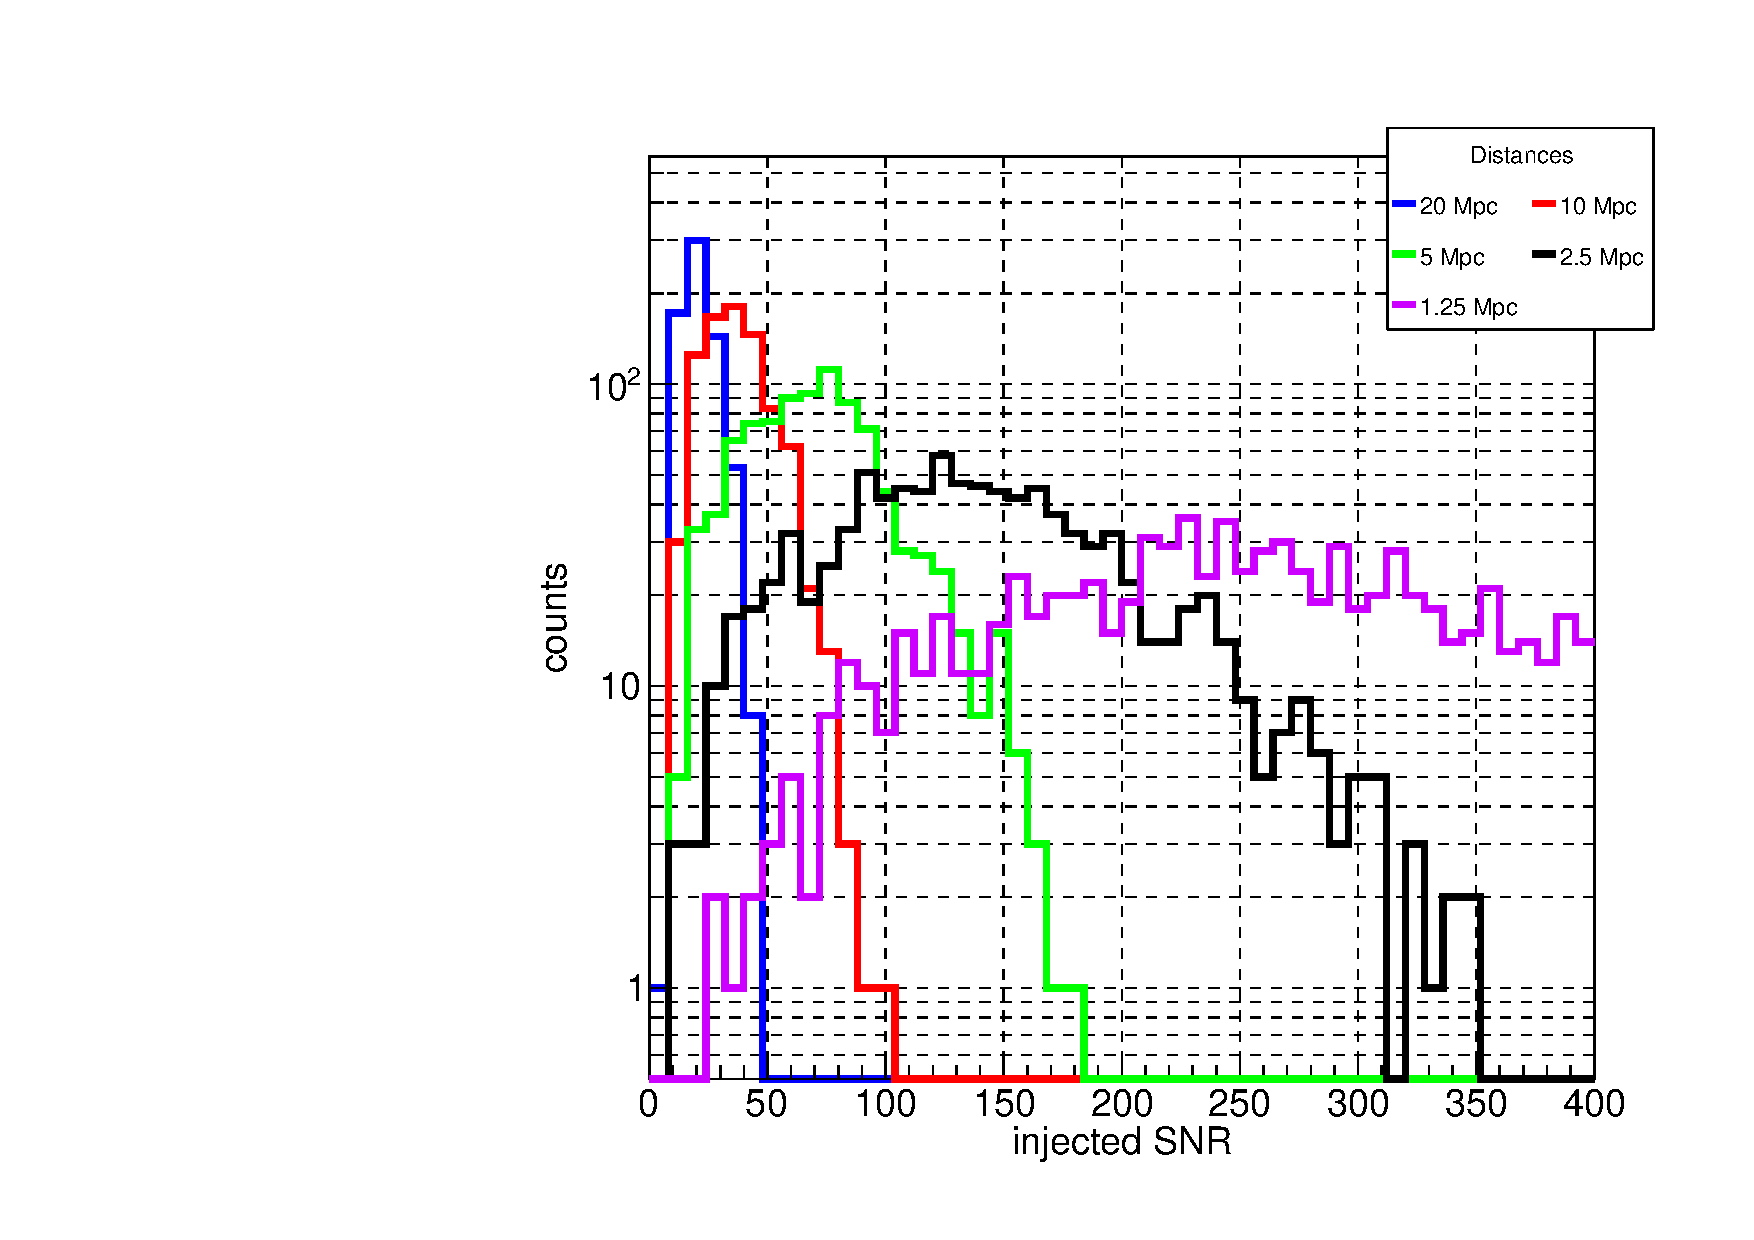
\includegraphics[width=.333333333333333333\textwidth]{figures/Capitolo_4/report/Network_iSNR_FactorsSHT2_0spin1.pdf}}
	\subfloat[][\emph{SHT2.2}]
	{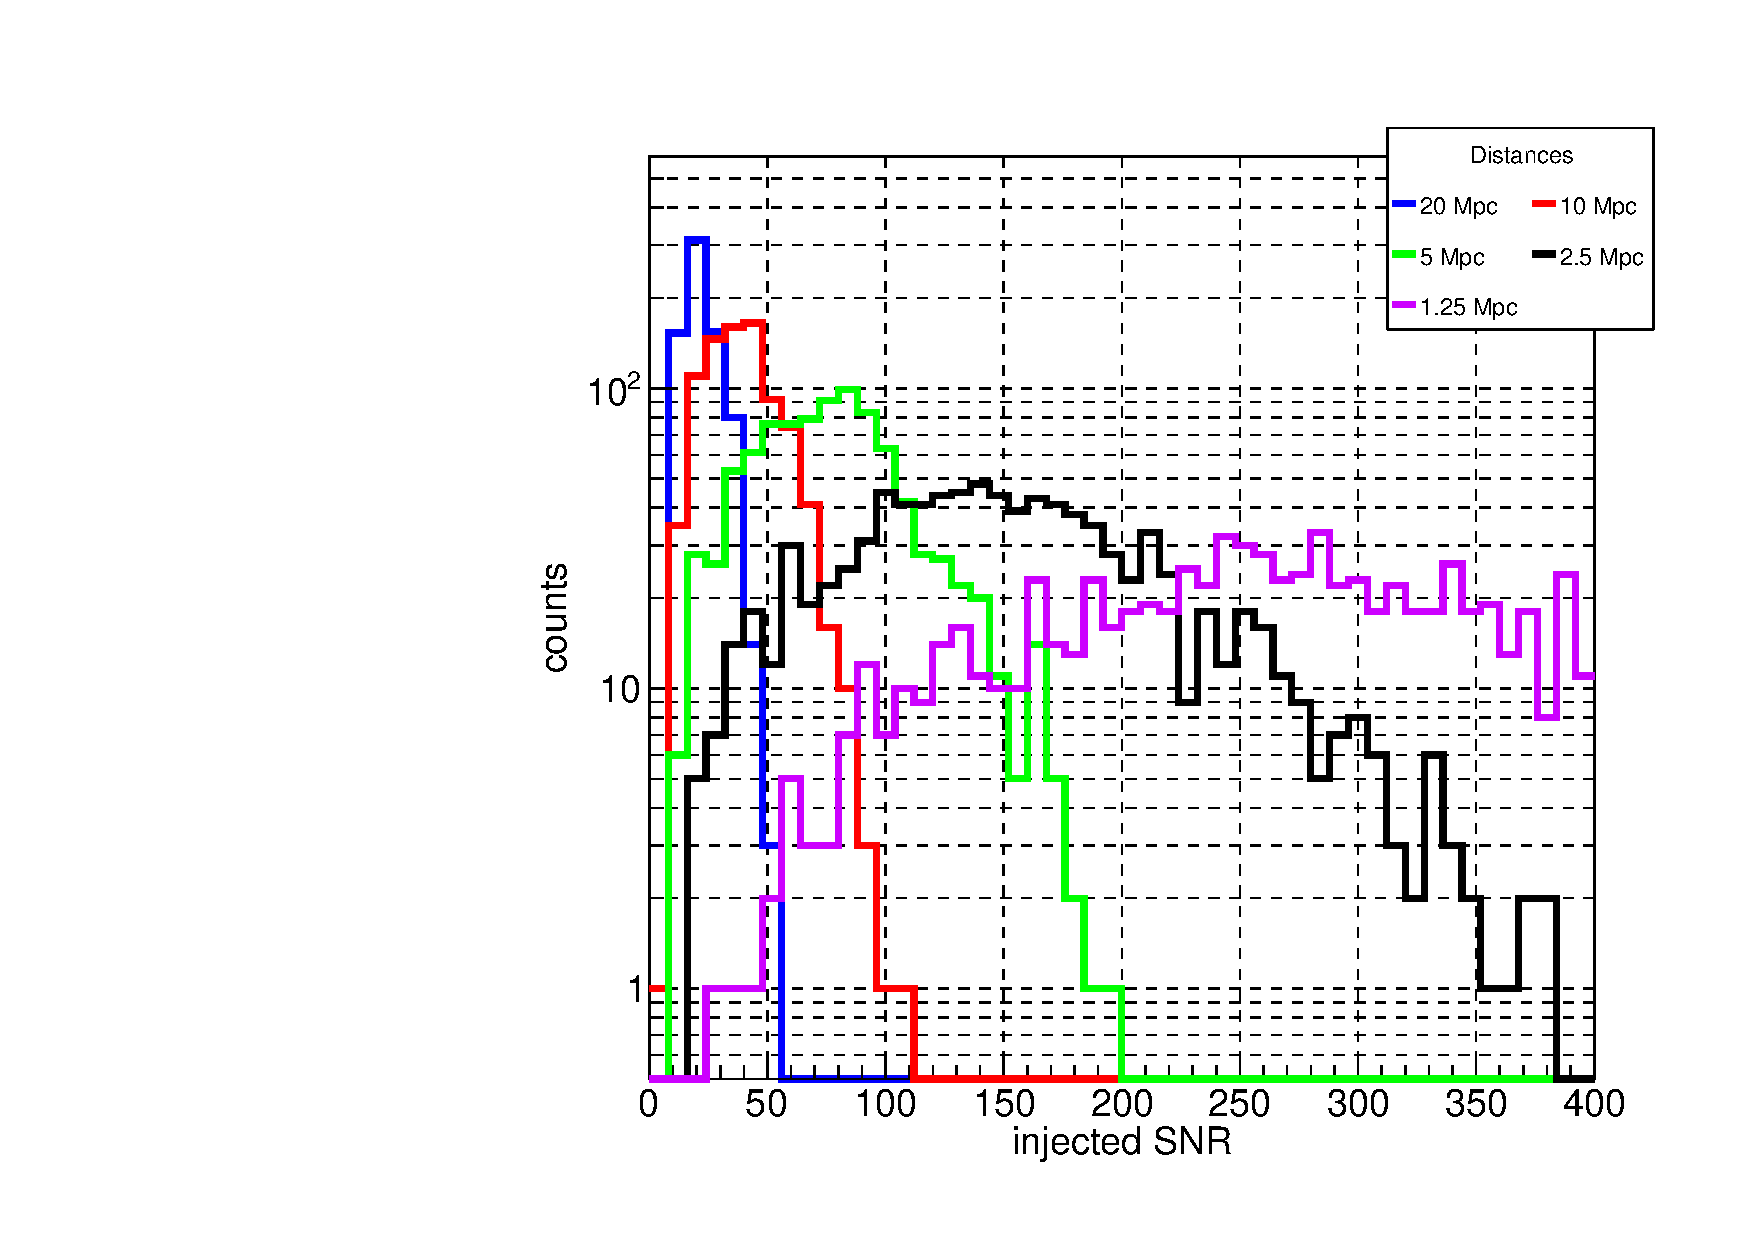
\includegraphics[width=.333333333333333333\textwidth]{figures/Capitolo_4/report/Network_iSNR_FactorsSHT2_2spin1.pdf}}
	\subfloat[][\emph{APR4}]
	{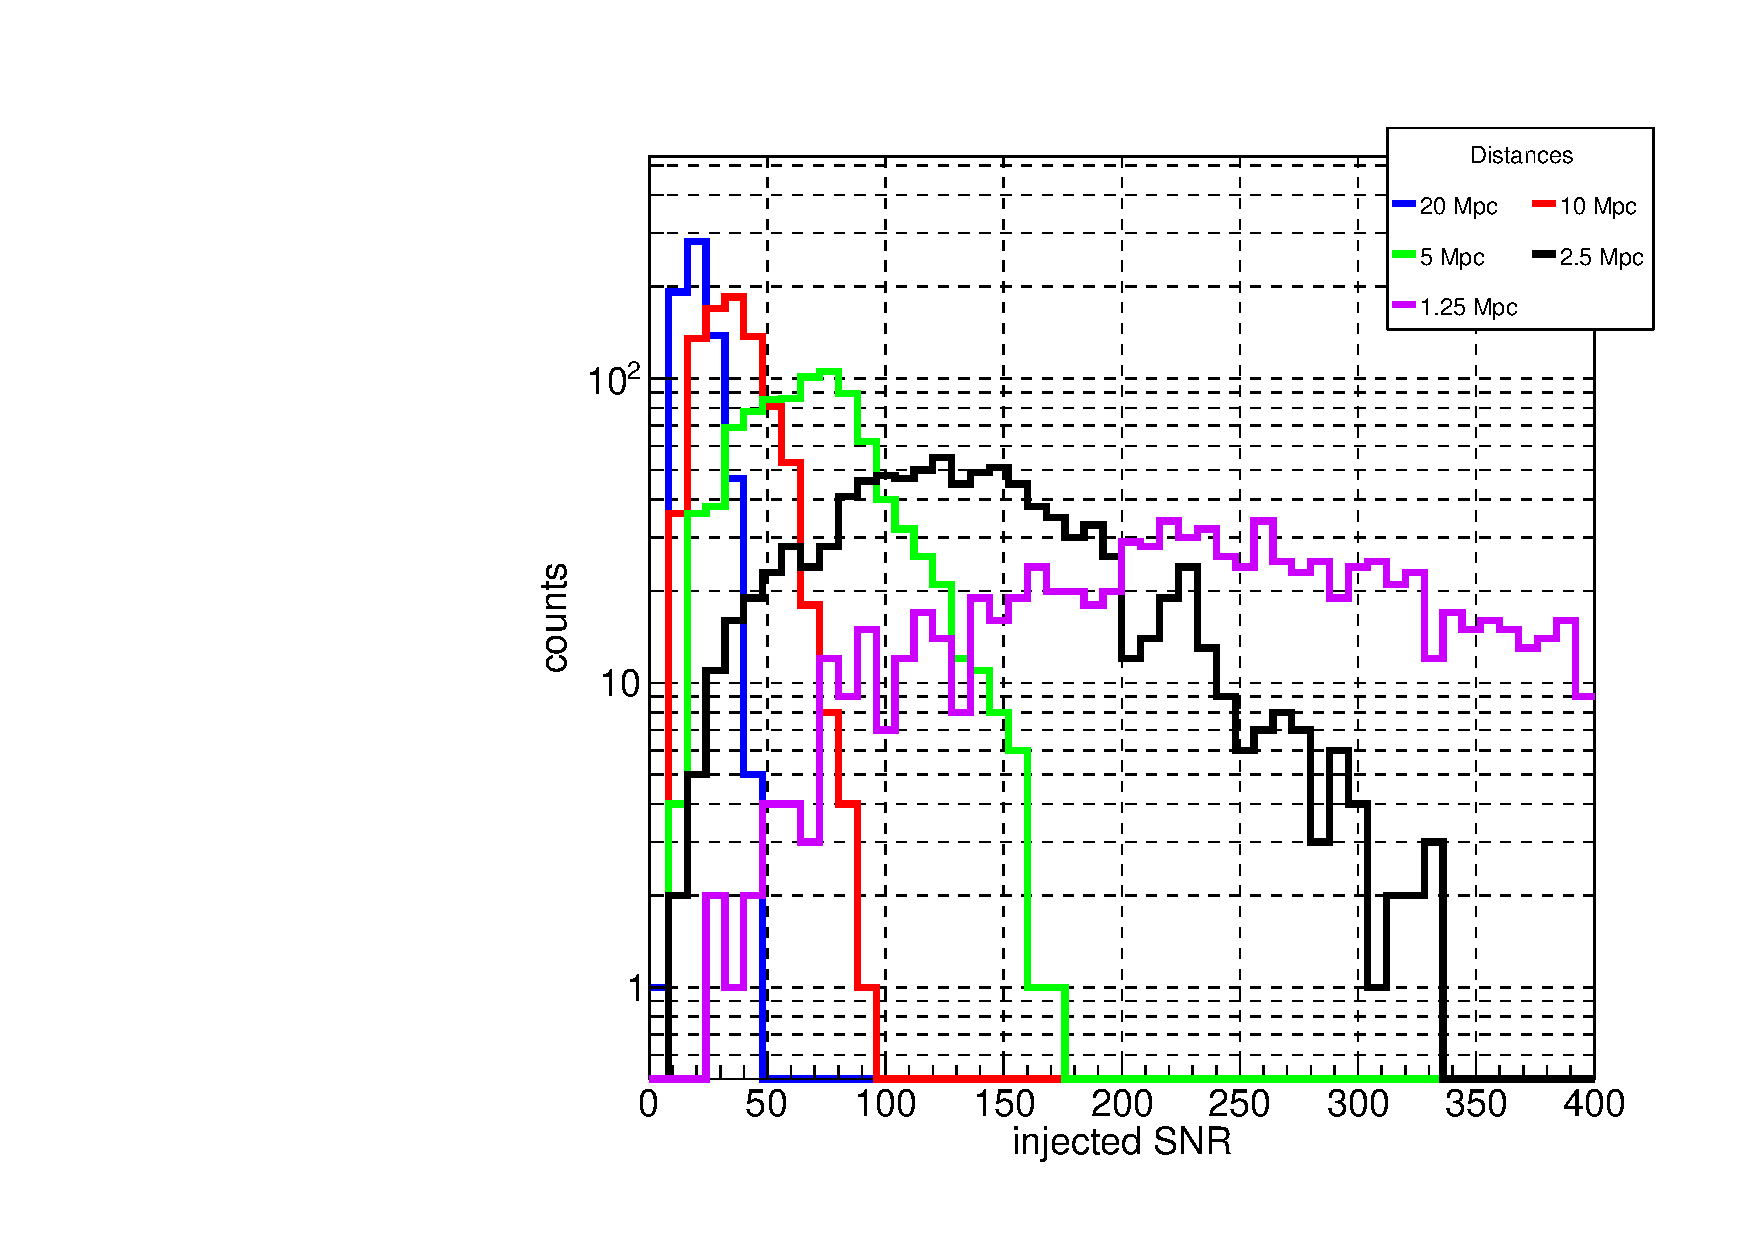
\includegraphics[width=.333333333333333333\textwidth]{figures/Capitolo_4/report/Network_iSNR_FactorsAPR4_q09.pdf}}
	\vspace{-5pt}
	\caption{SNR iniettato per le tre EOS, diviso nelle distanze}
	\label{fig:SNR_INJ_REC_COUNTS}
	\vspace{-15pt}
\end{figure}
Nella ricostruzione è necessario scegliere alcuni parametri soglia di cui si riportano i principali:
\begin{itemize}
	\item bbp: Black Pixel Probability, ovvero la soglia di eccesso di potenza per la selezione dei pixel nella mappa tempo-frequenza, impostata a 0.001;
	\item Tgap: ovvero la distanza in tempo tra due cluster di dati perché questi vengano ricostruiti come eventi separati, fissata a 0.2s;
	\item Fgap: ovvero la distanza in frequenza tra due cluster di dati perché questi vengano ricostruiti come eventi separati, fissata a 128Hz.
\end{itemize}

Gli eventi che vengono ricostruiti non sono tutti quelli iniettati, ma solo la parte di essi che viene rivelata con SNR sopra al valore di soglia nella rete. Si riportano in Figura \ref{fig:skyposrec} le distribuzioni degli eventi simulati che sono da confrontare con i grafici in Figura \ref{fig:skypos}. Si nota che il numero di eventi ricostruiti è minore (4298/4770), in particolare gli eventi la cui ricostruzione non avviene sono soprattutto gli eventi a distanza maggiore. Si nota poi dal grafico (b) come rispetto al corrispettivo negli iniettati vi siano evidenti buchi, che giustificano ulteriormente la mancata ricostruzione: esistono punti ciechi della rete. L'aggiunta nei prossimi run di altri rivelatori risolverà almeno in parte questa problematica. 
%che comunque non riguarda direttamente questa tesi, che non si impegna a valutare l'efficienza del network, ma l'efficienza dell'algoritmo cWB.
\begin{figure}[ht]
	\vspace{-20pt}
	\centering
	\subfloat[][\emph{Distribuzione distanze}]
	{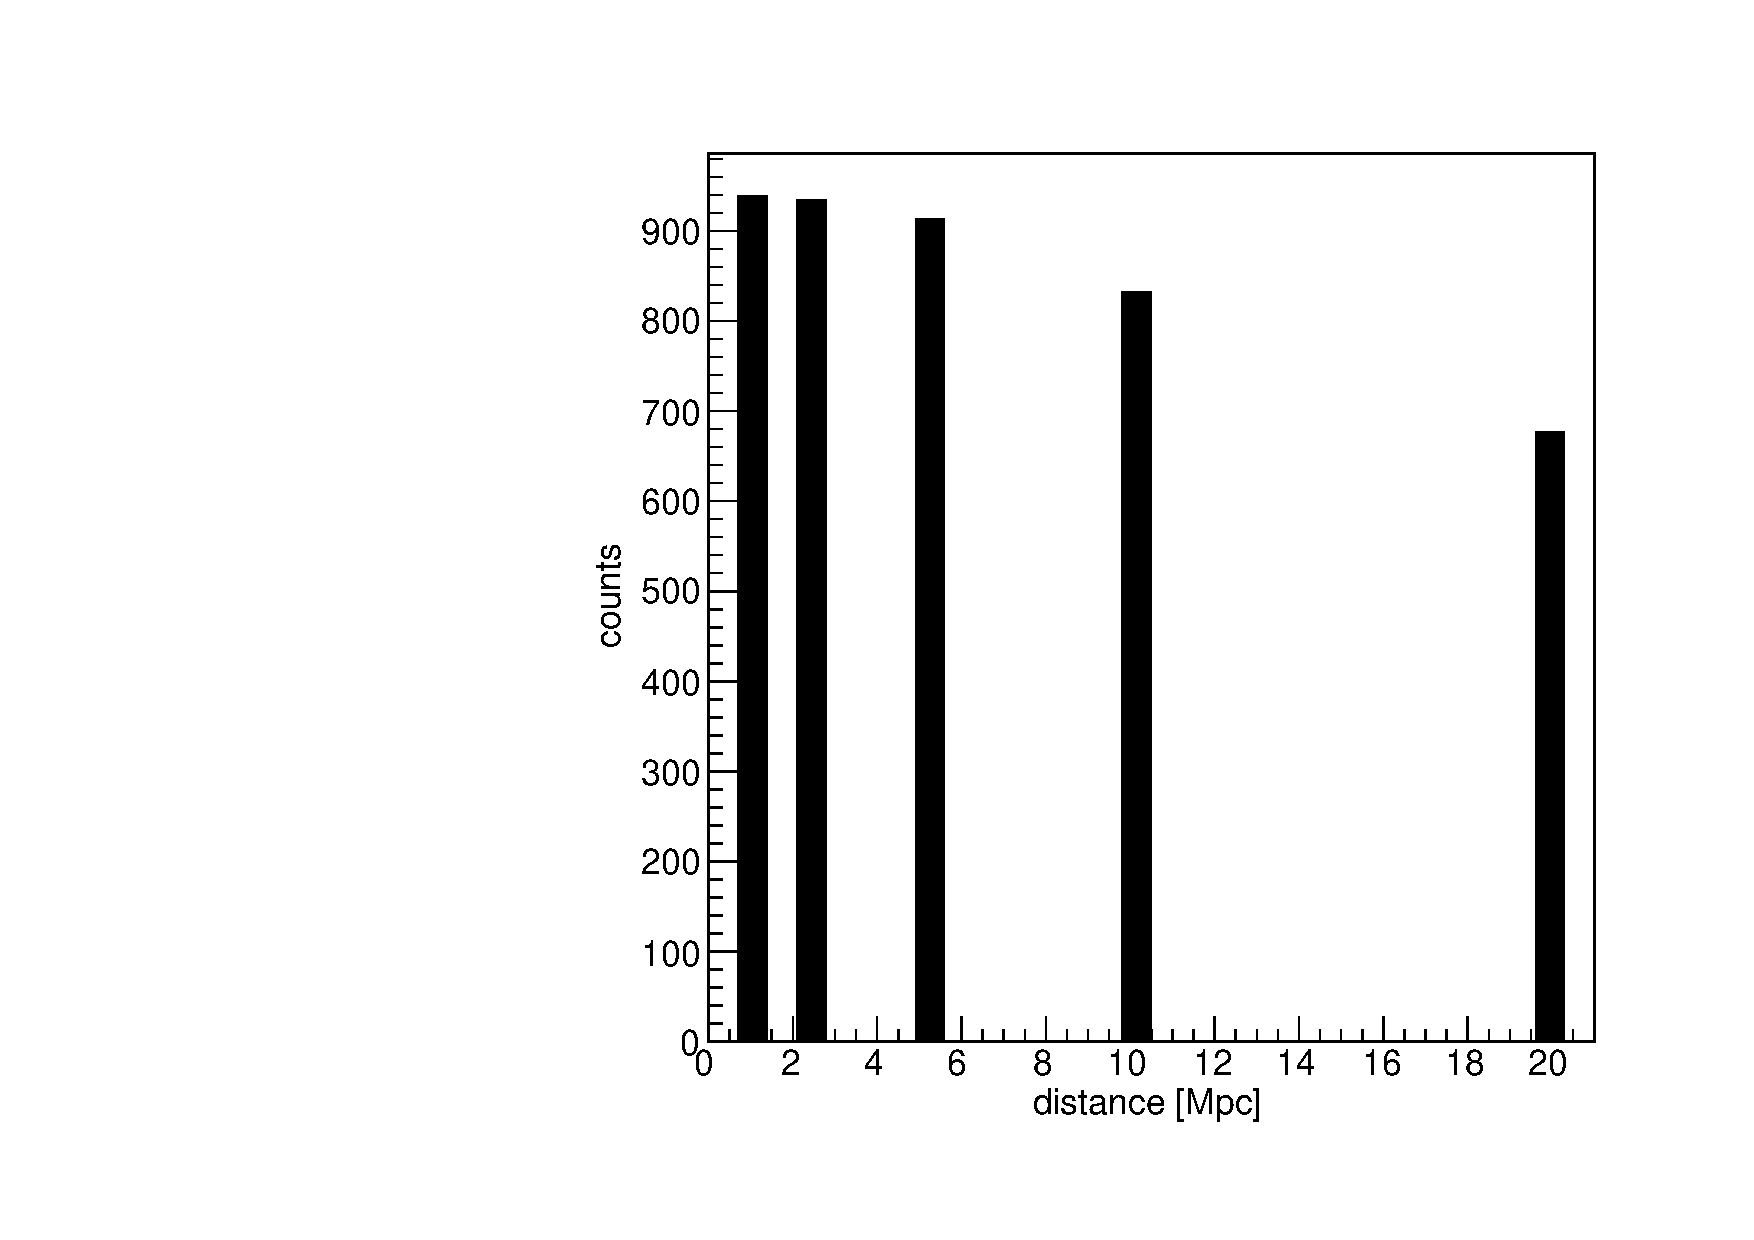
\includegraphics[width=.3\textwidth]{figures/Capitolo_4/report/RfactorsSHT2_0spin1.pdf}}\quad
	\subfloat[][\emph{Distribuzione celeste}]
	{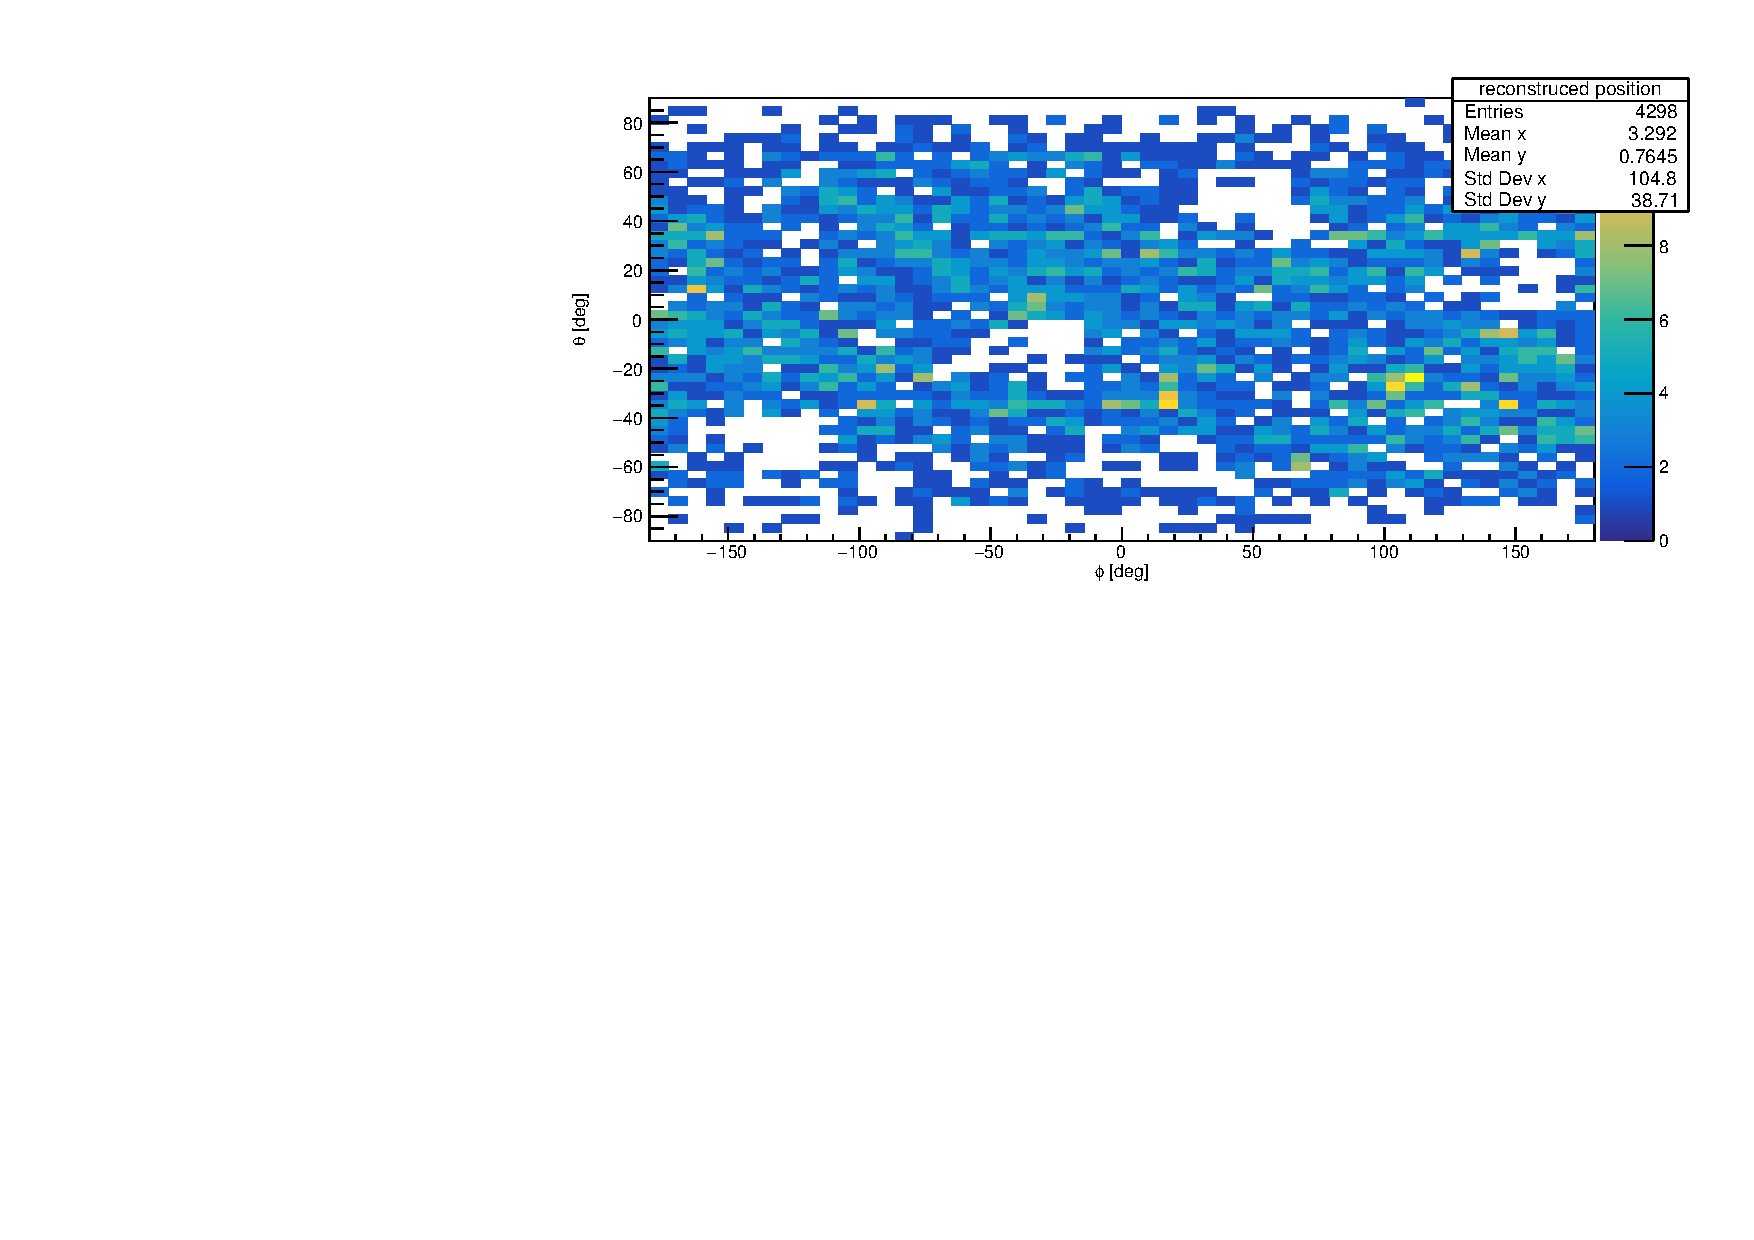
\includegraphics[width=.6\textwidth]{figures/Capitolo_4/report/RopositionSHT2_0spin1.pdf}}
	\vspace{-5pt}
	\caption{Distribuzione degli eventi ricostruiti per l'EOS SHT2.0}
	\label{fig:skyposrec}
	\vspace{-10pt}
\end{figure}
%Si riportano gli istogrammi per gli SNR iniettati e ricostruiti dal network, divisi per distanza della sorgente. Si può notare come al crescere della distanza le distribuzioni siano sempre più schiacciate a SNR bassi.
%\begin{figure}[ht]
%	\vspace{-20pt}
%	\centering
%	\subfloat[][\emph{SHT2.0}]
%	{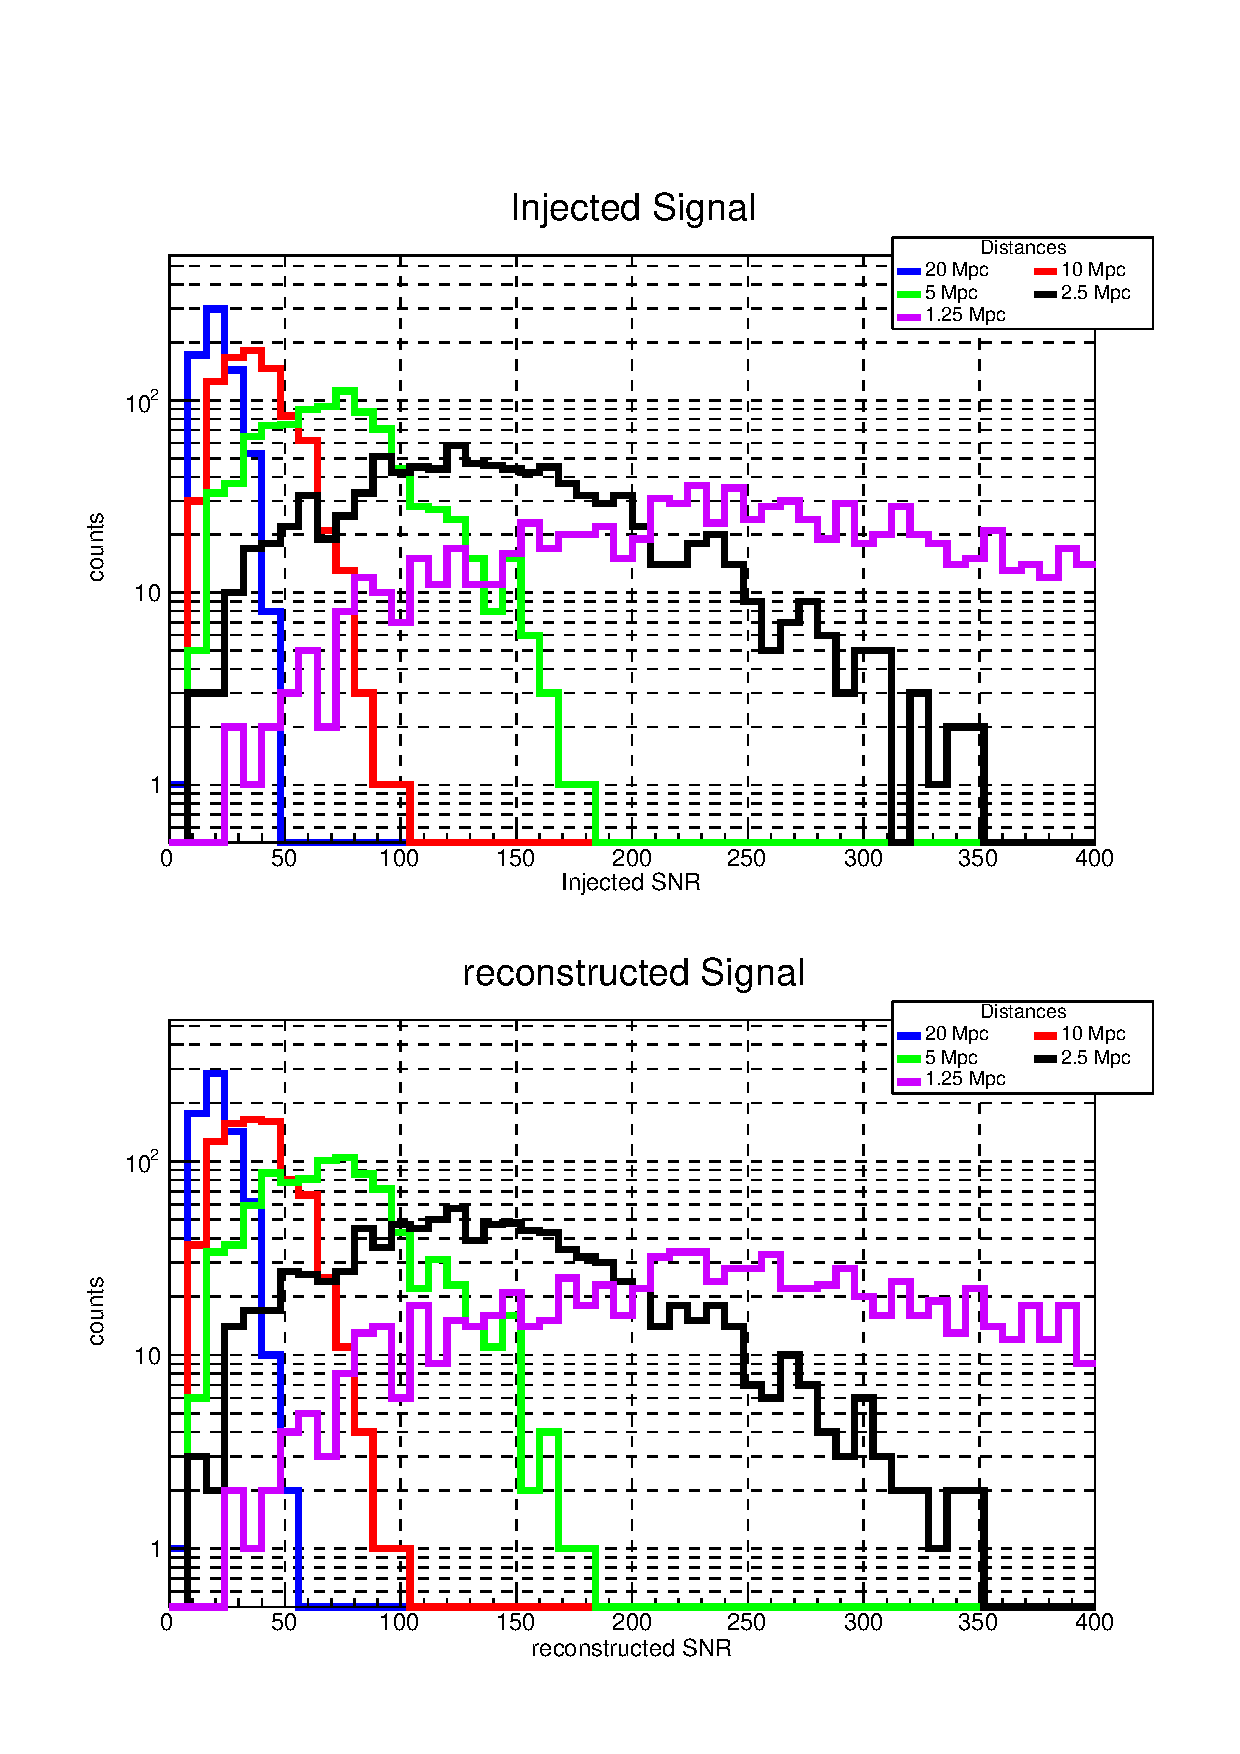
\includegraphics[width=.333333333333333333\textwidth]{figures/Capitolo_4/report/Network_SNR_FactorsSHT2_0spin1.pdf}}
%	\subfloat[][\emph{SHT2.2}]
%	{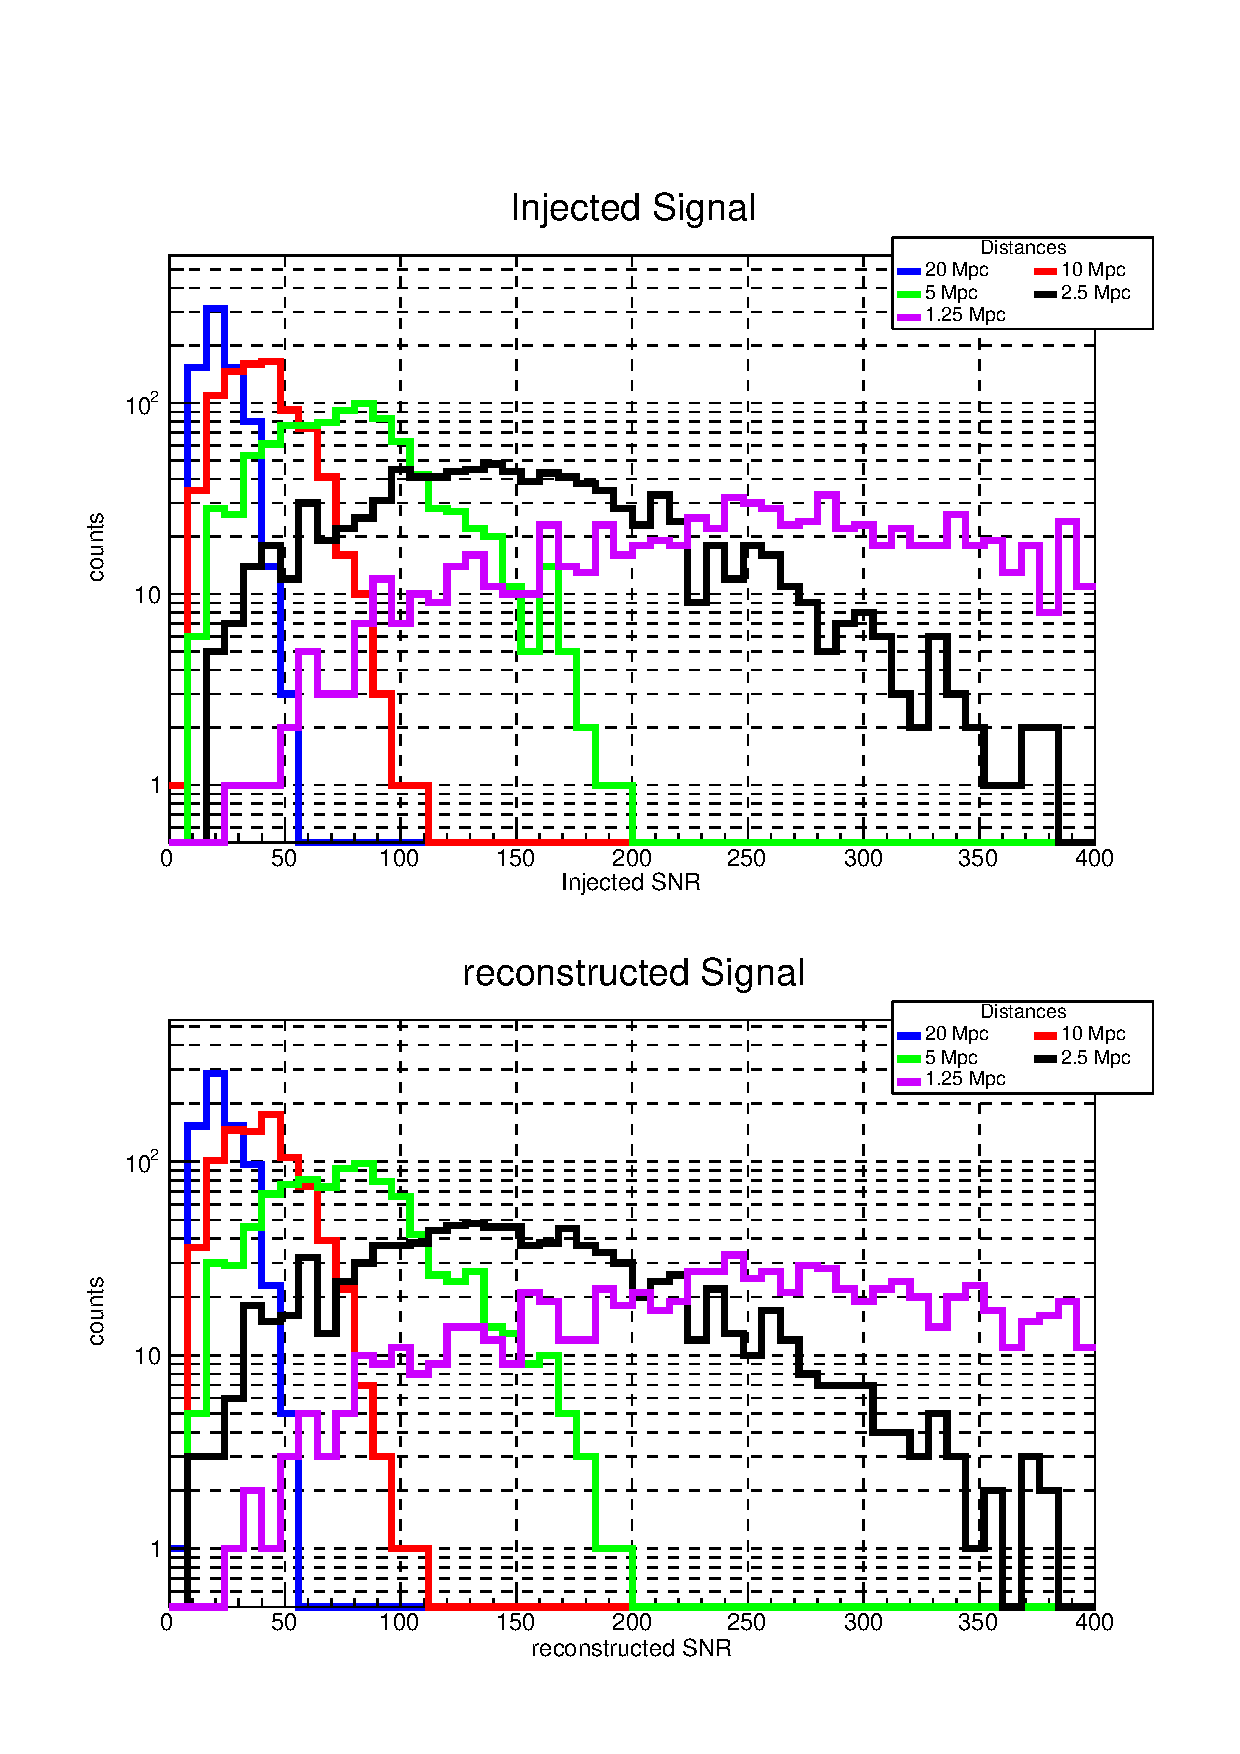
\includegraphics[width=.333333333333333333\textwidth]{figures/Capitolo_4/report/Network_SNR_FactorsSHT2_2spin1.pdf}}
%	\subfloat[][\emph{APR4}]
%	{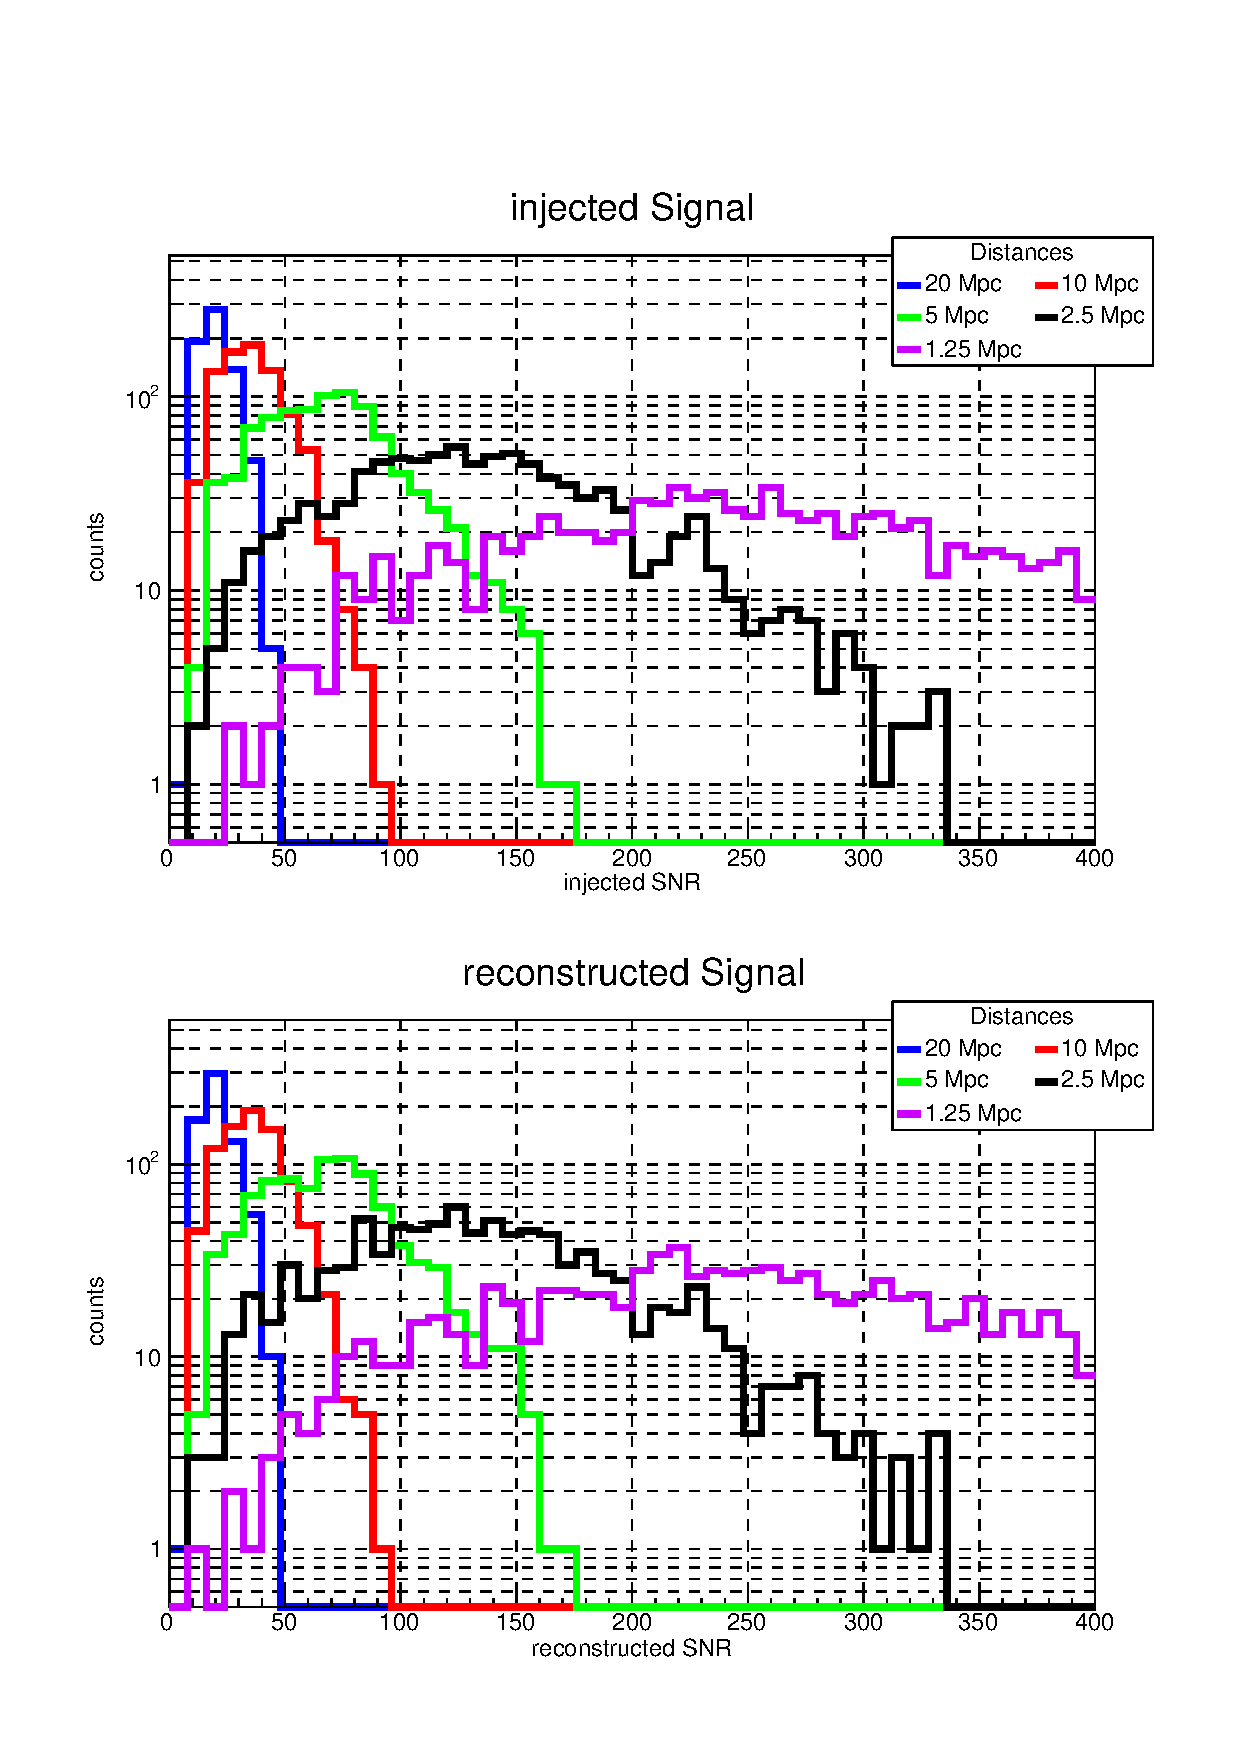
\includegraphics[width=.333333333333333333\textwidth]{figures/Capitolo_4/report/Network_SNR_FactorsAPR4_q09.pdf}}
%	\vspace{-5pt}
%	\caption{SNR iniettato (sopra) e ricostruito (sotto) per le due EOS}
%	\label{fig:SNR_INJ_REC_COUNTS}
%	\vspace{-15pt}
%\end{figure}
Si procede quindi a verificare in modo quantitativo l'efficienza dell'algoritmo di ricostruizione, facendo un fit degli SNR ricostruiti in funzione degli SNR iniettati. L'andamento ideale che ci si aspetta è rappresentato dalla bisettrice del primo e terzo quadrante, che corrisponde a una processo tale per cui l'SNR ricostruito è pari a quello iniettato.
%\begin{figure}[H]
%	\vspace{-10pt}
%	\centering
%	\subfloat[][\emph{SHT2}]
%	{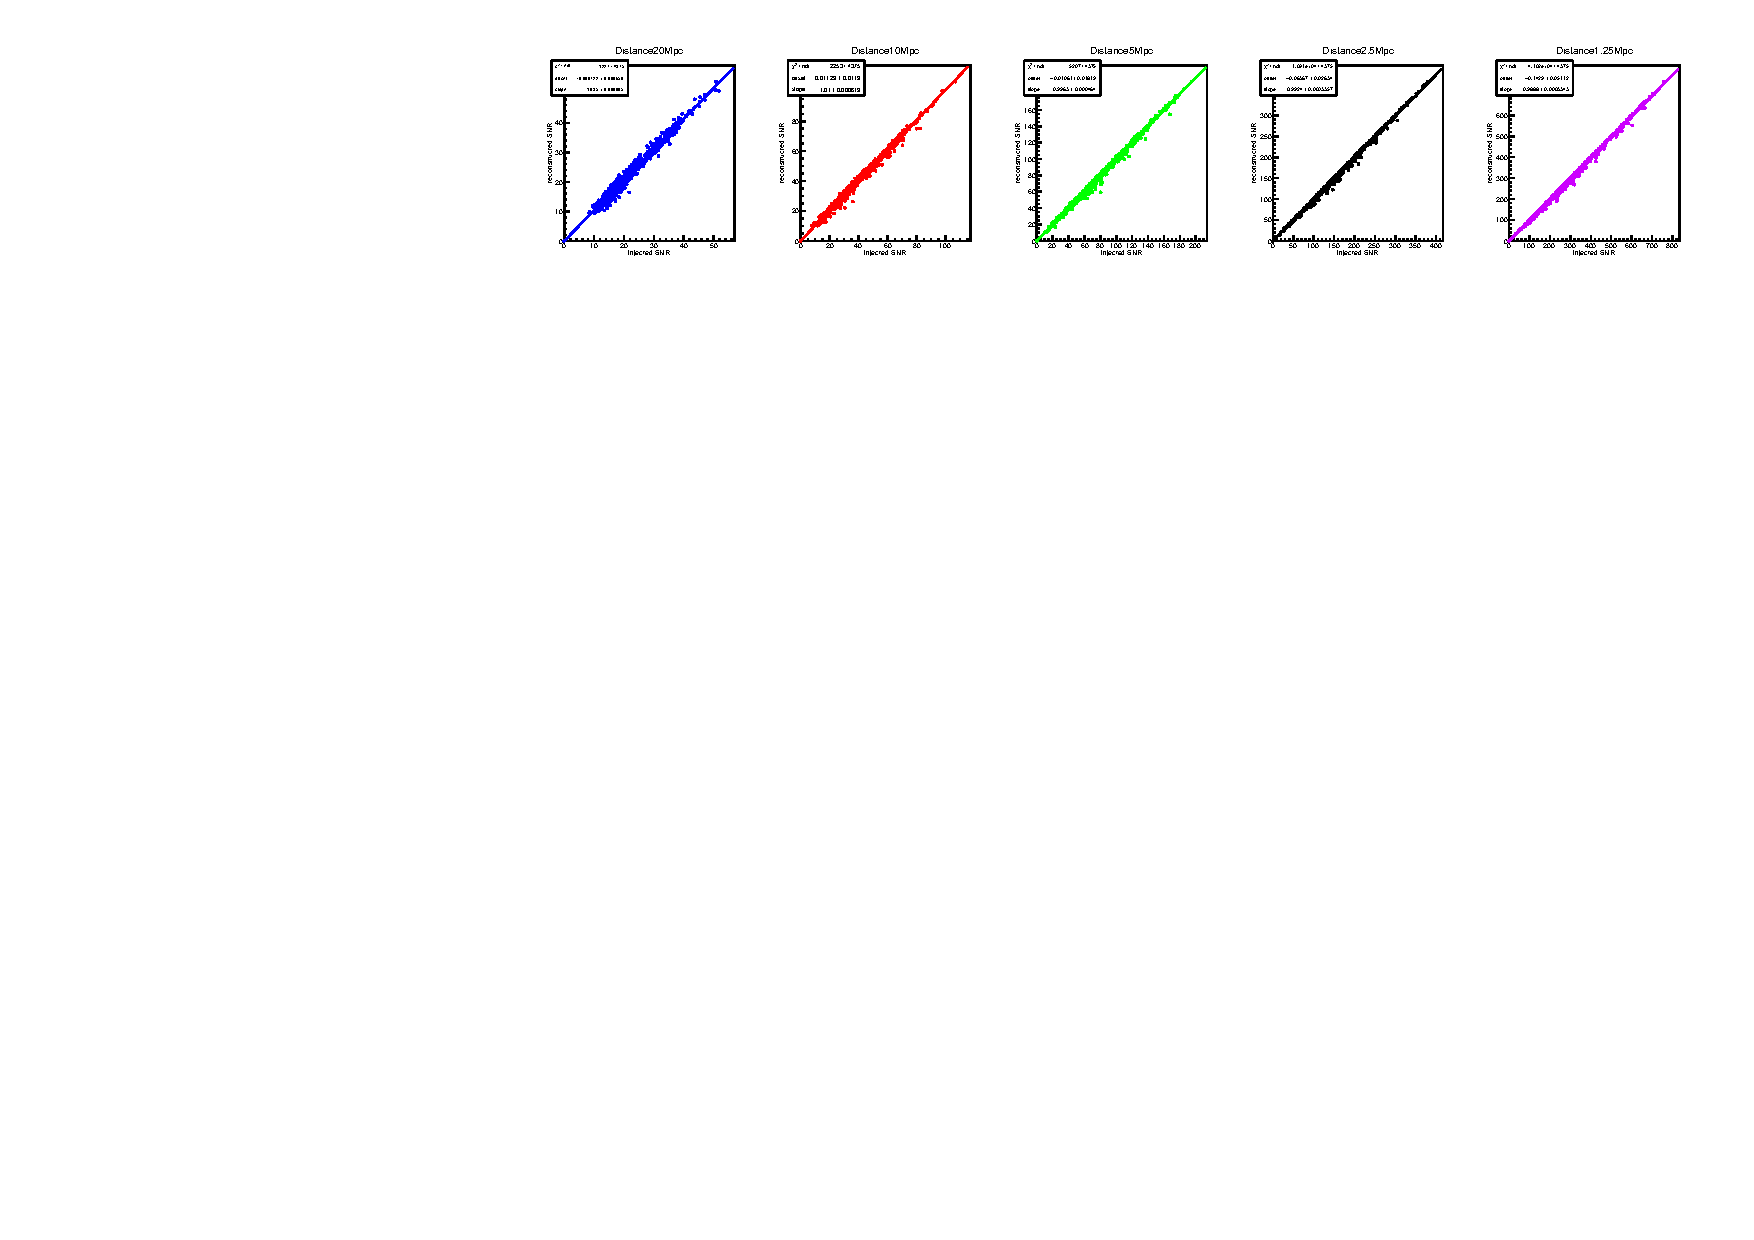
\includegraphics[width=1\textwidth]{figures/Capitolo_4/FITSHT2_0spin1.pdf}} \\
%	\vspace{-10pt}
%	\subfloat[][\emph{APR4}]
%	{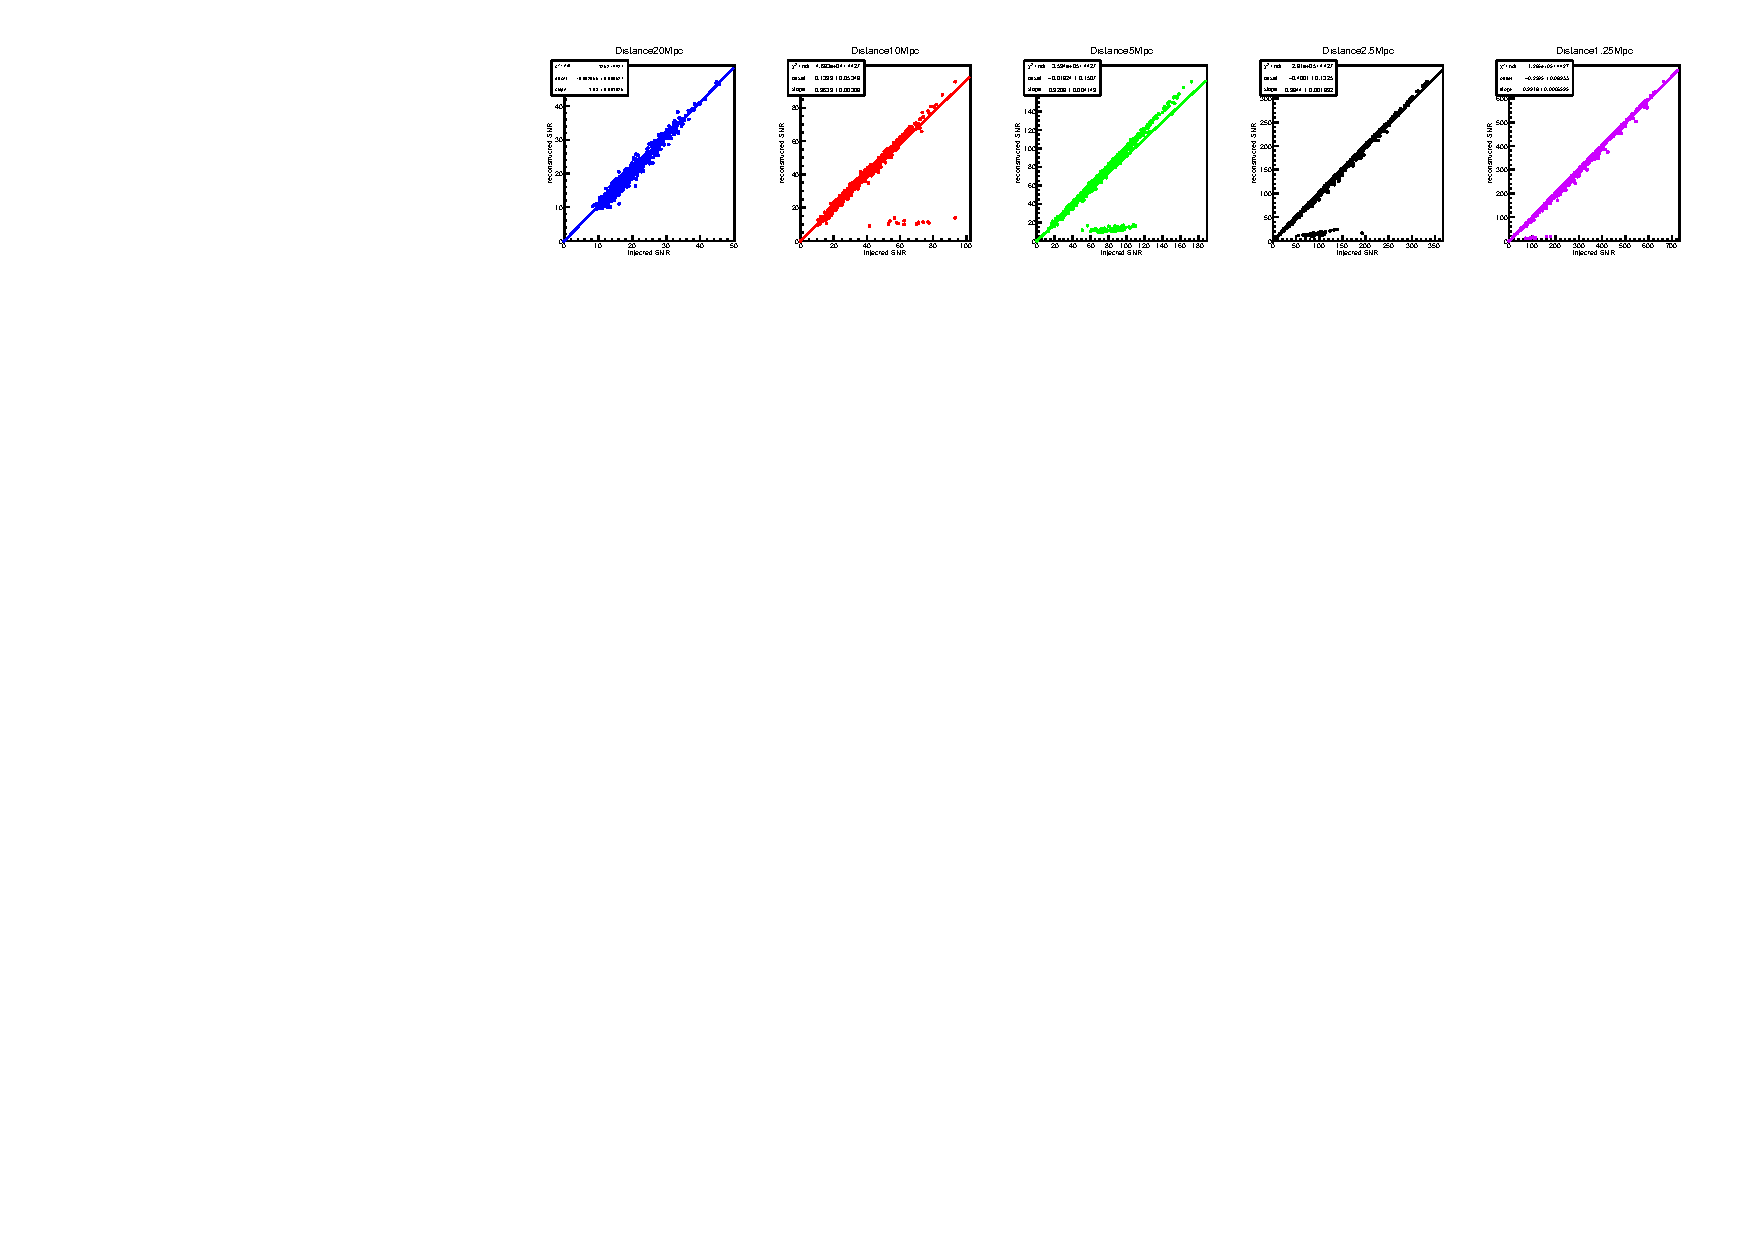
\includegraphics[width=1\textwidth]{figures/Capitolo_4/FITAPR4_q09.pdf}}
%	\vspace{-5pt}
%	\caption{Fit dell'SNR ricostruito in funzione dell'SNR iniettato per le due EOS}
%	\label{fig:overlap}
%	\vspace{-15pt}
%\end{figure}
\begin{figure}[ht]
	\vspace{-10pt}
	\centering
	\subfloat[][\emph{SHT2.0}]
	{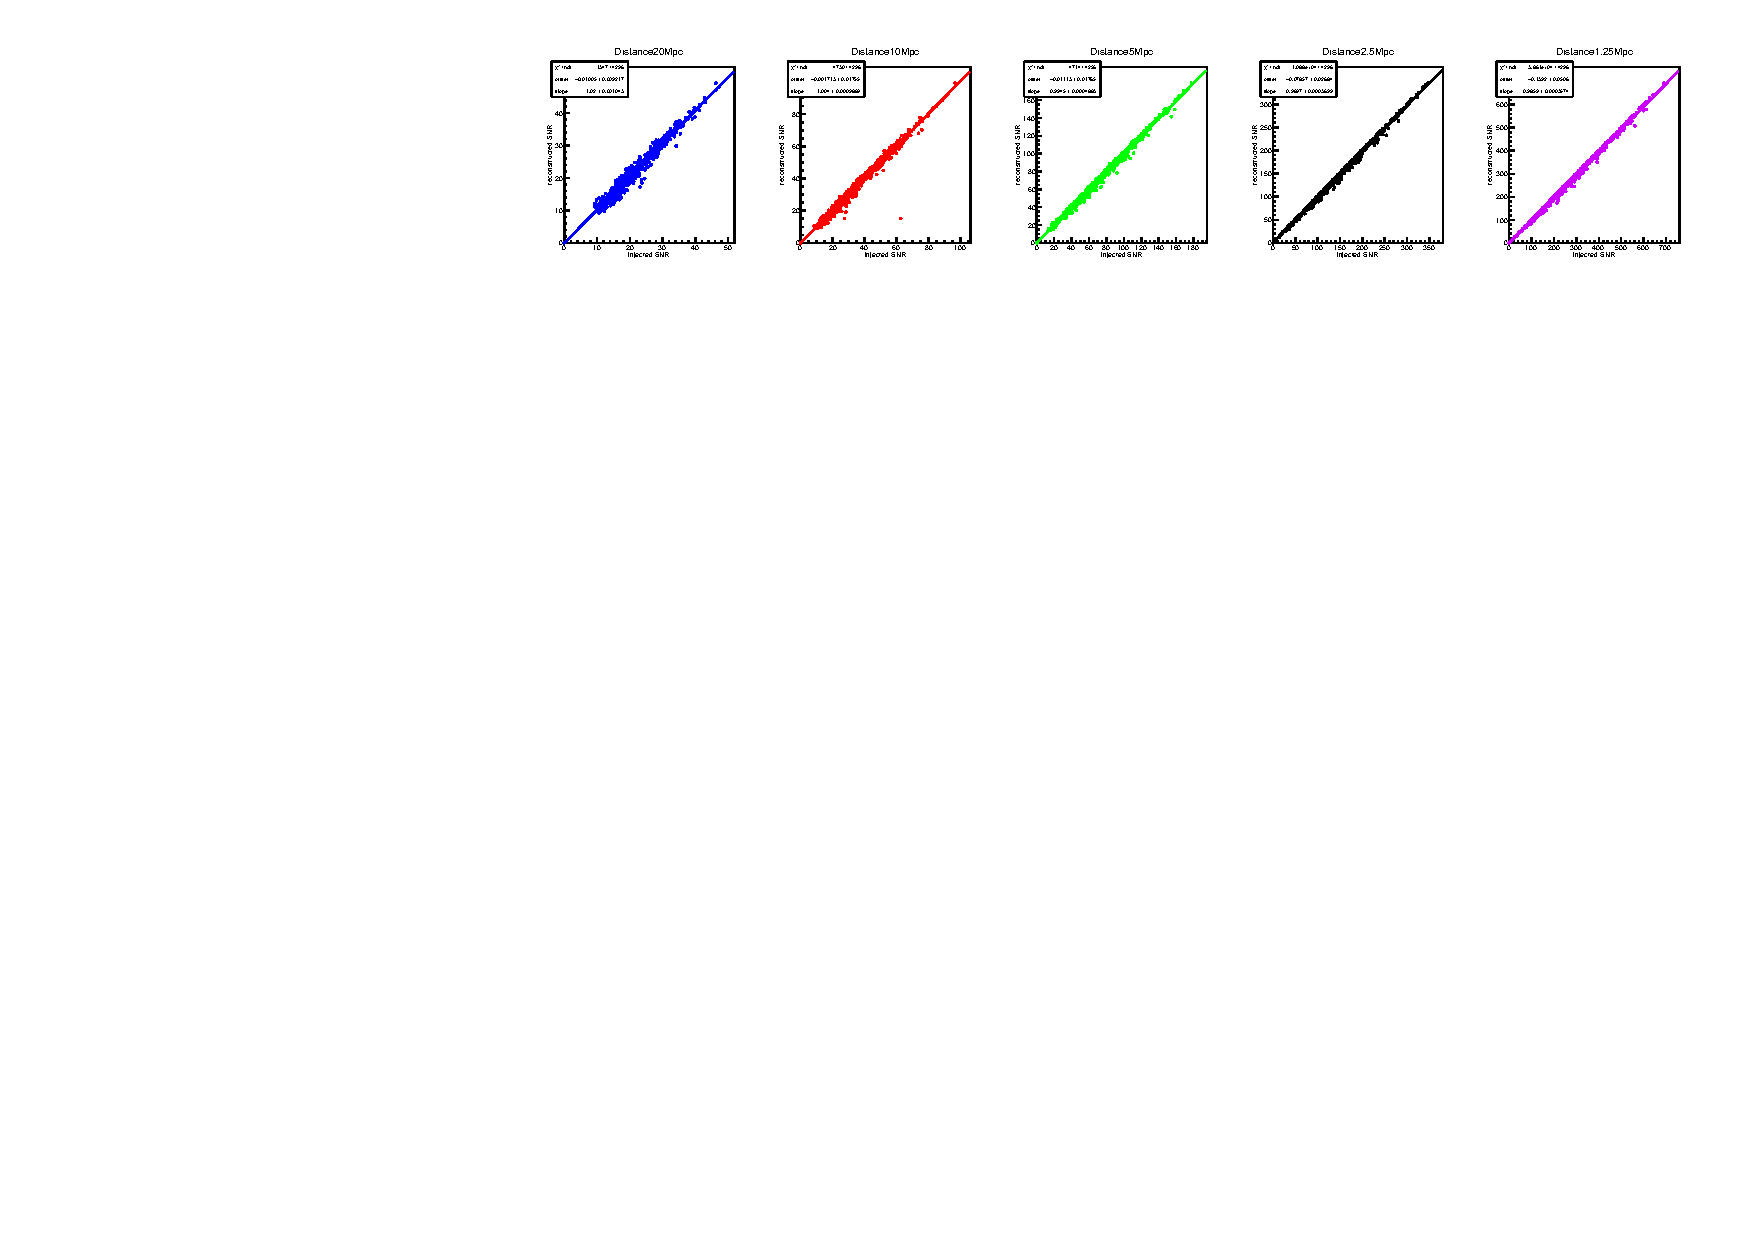
\includegraphics[width=1\textwidth]{figures/Capitolo_4/report/FITSHT2_0spin1.pdf}} \\
	\vspace{-10pt}
	\subfloat[][\emph{SHT2.2}]
	{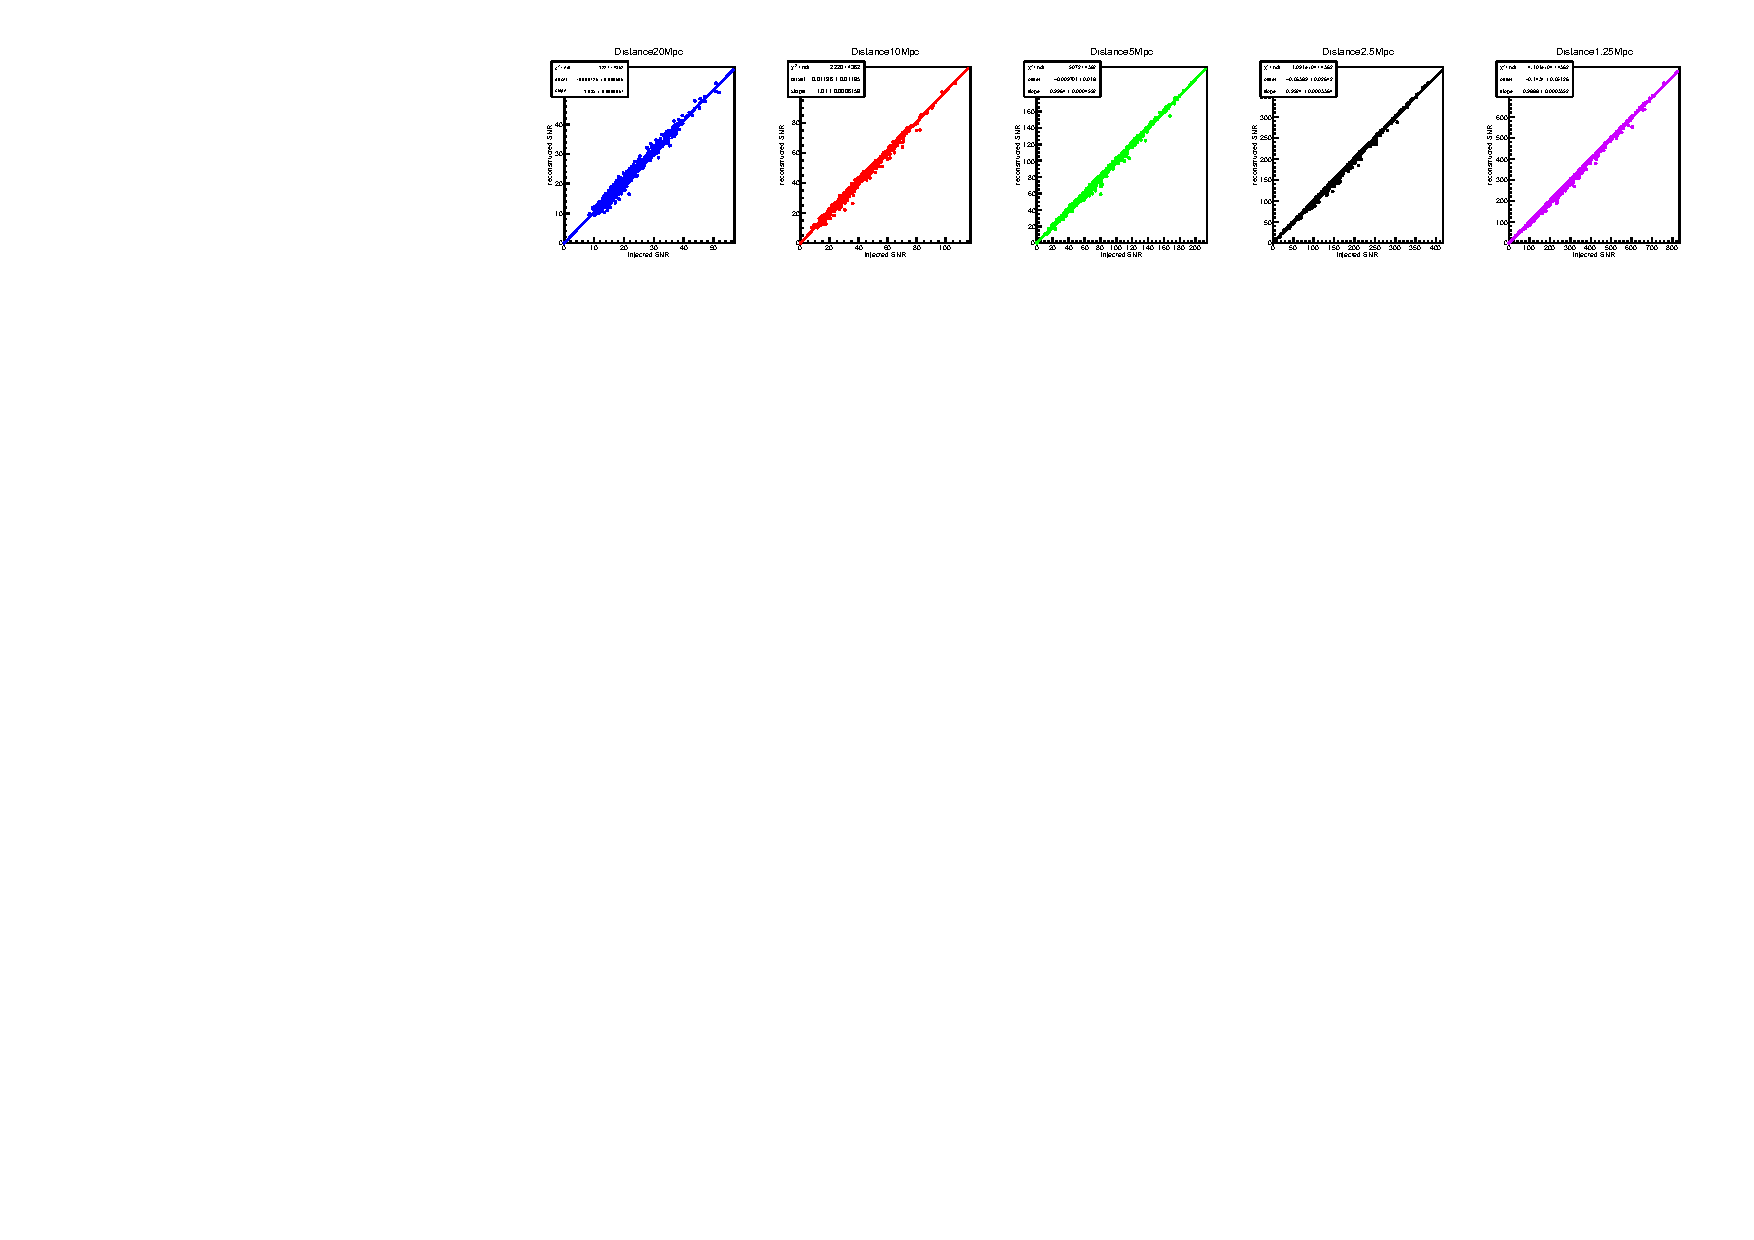
\includegraphics[width=1\textwidth]{figures/Capitolo_4/report/FITSHT2_2spin1.pdf}}\\
	\vspace{-10pt}
	\subfloat[][\emph{APR4}]
	{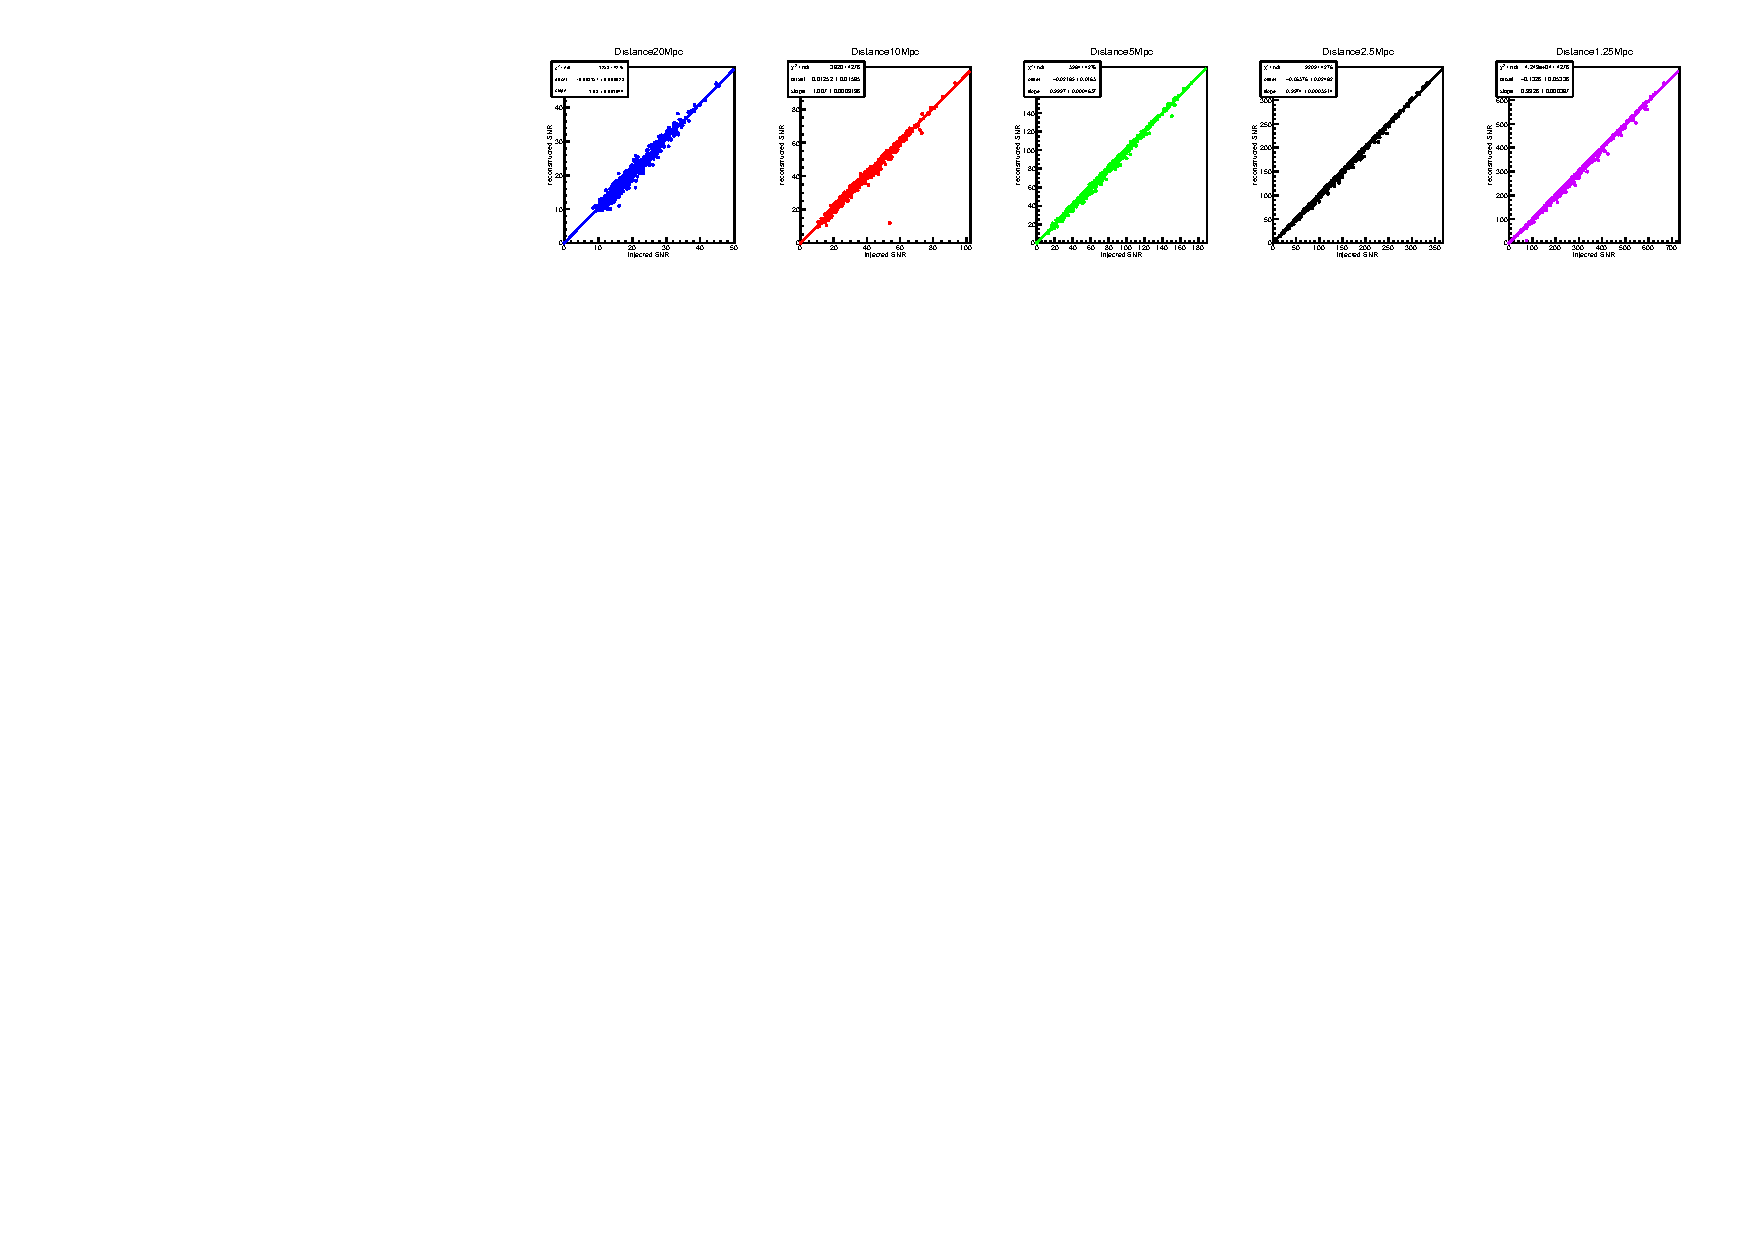
\includegraphics[width=1\textwidth]{figures/Capitolo_4/report/FITAPR4_q09.pdf}}\\
	\vspace{-8pt}
	\caption{Fit dell'SNR ricostruito in funzione dell'SNR iniettato per le due EOS}
	\label{fig:overlap}
	\vspace{-10pt}
\end{figure}
Si può notare come le ricostruzioni siano generalmente vicine a tale condizione. È possibile osservare una sistematicità nella ricostruzione, che risulta leggermente sovrastimata a SNR bassi, quindi per grandi distanze, dove si ha $slope > 1$, mentre per SNR elevati vi è una sottostima, producendo $slope < 1$. Si osserva inoltre che non c'è offset significativo risultando sempre compatibile con il passaggio per l'origine secondo il critero dei $3\sigma$.

Si riportano quindi gli overlap in funzione degli SNR ricostruiti. In particolare si ha che denotando il segnale iniettato e ricostruito per ogni rivelatore come $x_{I}[i]= [x_{I,1}, \dots x_{I,N}]$ e $x_{R}[i]= [x_{R,1}, \dots x_{R,N}]$ rispettivamente, si definiranno allora SNR iniettato e ricostruito come
%\vspace{-25pt}
\begin{equation}
%	\vspace{  -25pt}
	iSNR = \sum_{i=1}^{N}x_{I, i}^2 = |x_{I}|^2 \quad\quad\quad oSNR = \sum_{i=1}^{N}x_{R, i}^2 = |x_{R}|^2
	\label{eqn:iSNR_oSNR}
\end{equation} 
Esiste però un'altra quantità che si ottiene incrociando questi dati, definita come $ioSNR = \sum_{i=1}^{N}x_{I, i}x_{R, i}$, ovvero la correlazione incrociata, a ritardo temporale nullo, della forma d'onda iniettata e ricostruita. Grazie a questa quantità è possibile calcolare due grandezze fondamentali: l'energia residua $E_{res}= \sum_{i=1}^{N}(x_{R, i}-x_{I, i})^2 = oSNR + iSNR - 2ioSNR$, in Figura \ref{fig:residual_energy}, e l'$o_{verlap} = \frac{\braket{x_I}{x_R}}{\sqrt{|x_I||x_R|}} = \frac{ioSNR}{\sqrt{|x_I||x_R|}}$, in Figura \ref{fig:Overlap_SHT2_APR4}, che descrive la corrispondenza del segnale iniettato rispetto a quello ricostruito, in particolare per $o_{verlap}=1$ i due segnali hanno un matching perfetto, per $o_{verlap}=0$ invece non c'è ricostruzione del segnale.
%\begin{figure}[H]
%	\vspace{-20pt}
%	\centering
%	\subfloat[][\emph{SHT2}]
%	{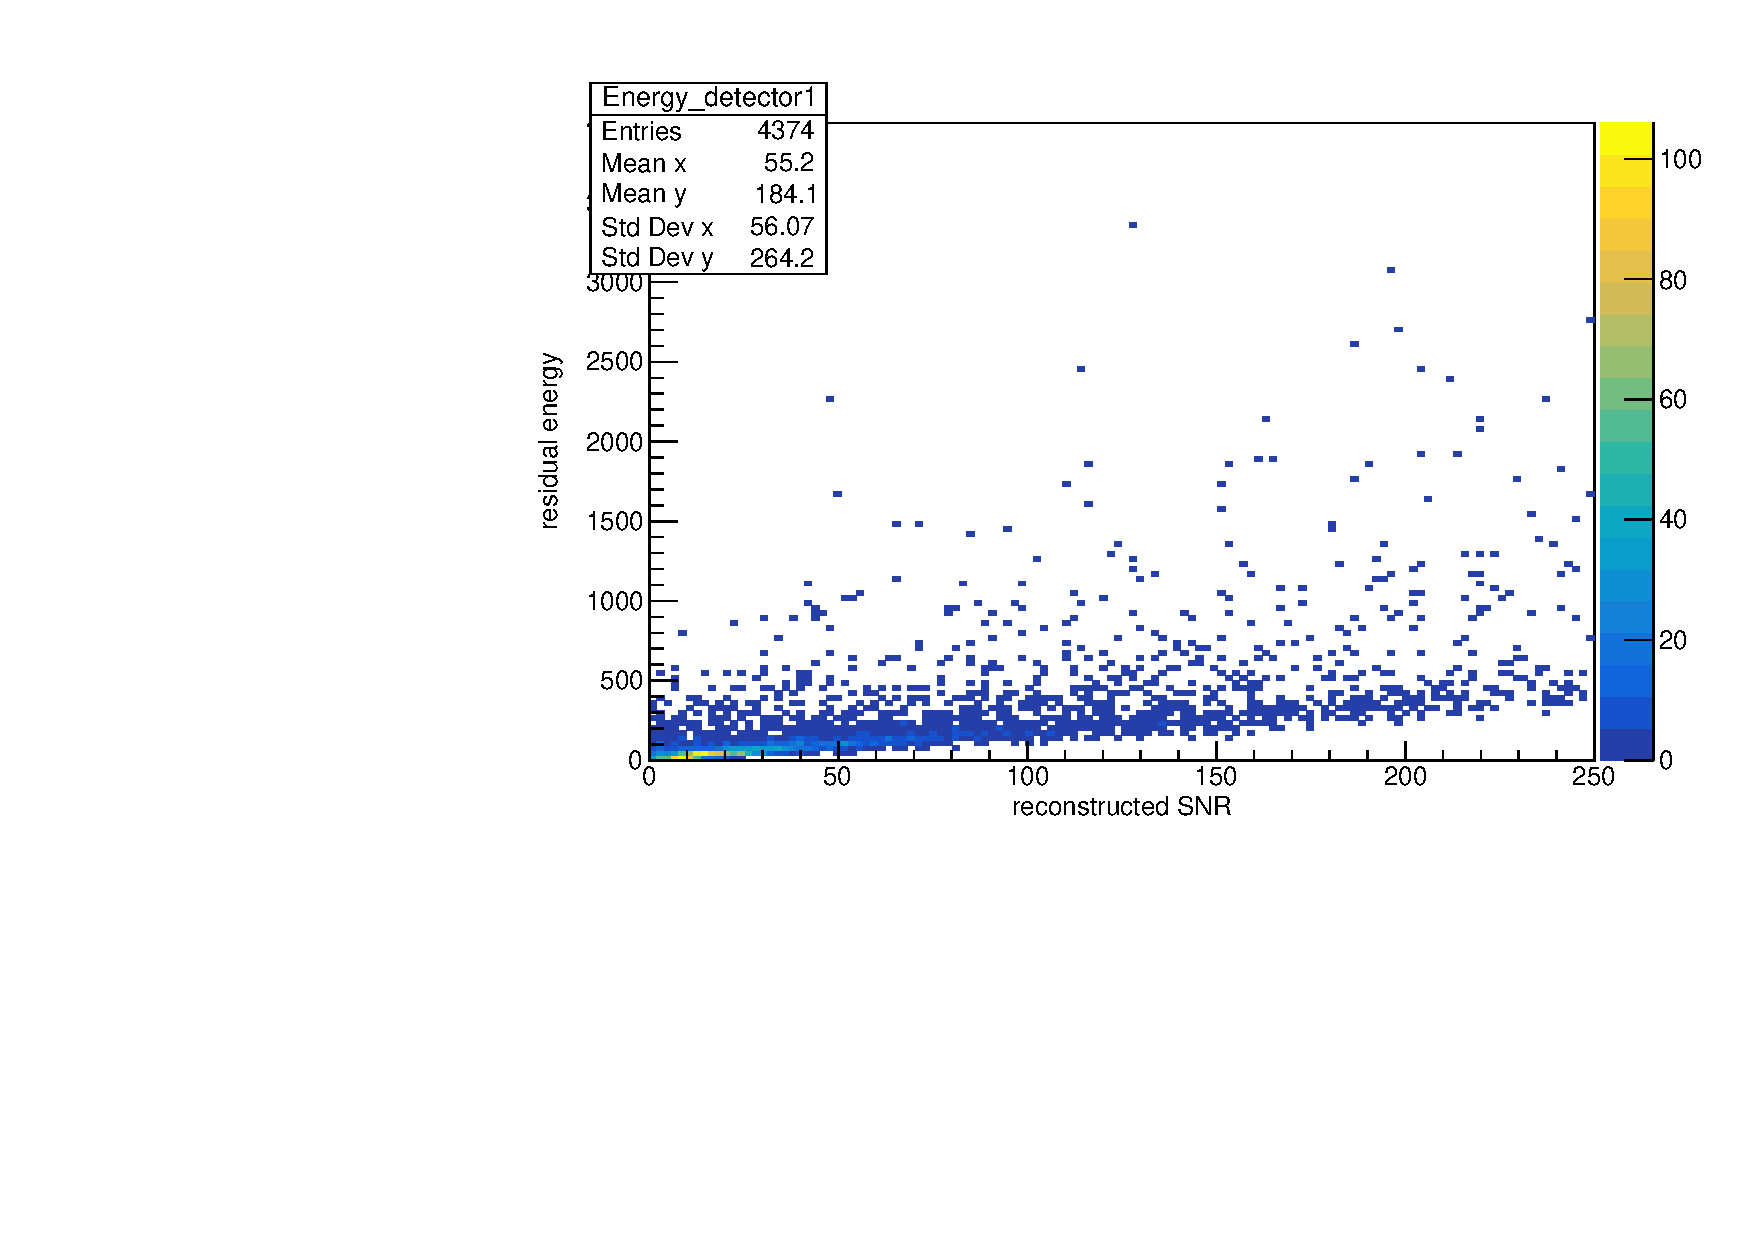
\includegraphics[width=.5\textwidth]{figures/Capitolo_4/EnergyDistributionDetector1SHT2_0spin1.pdf}}
%	\subfloat[][\emph{APR4}]
%	{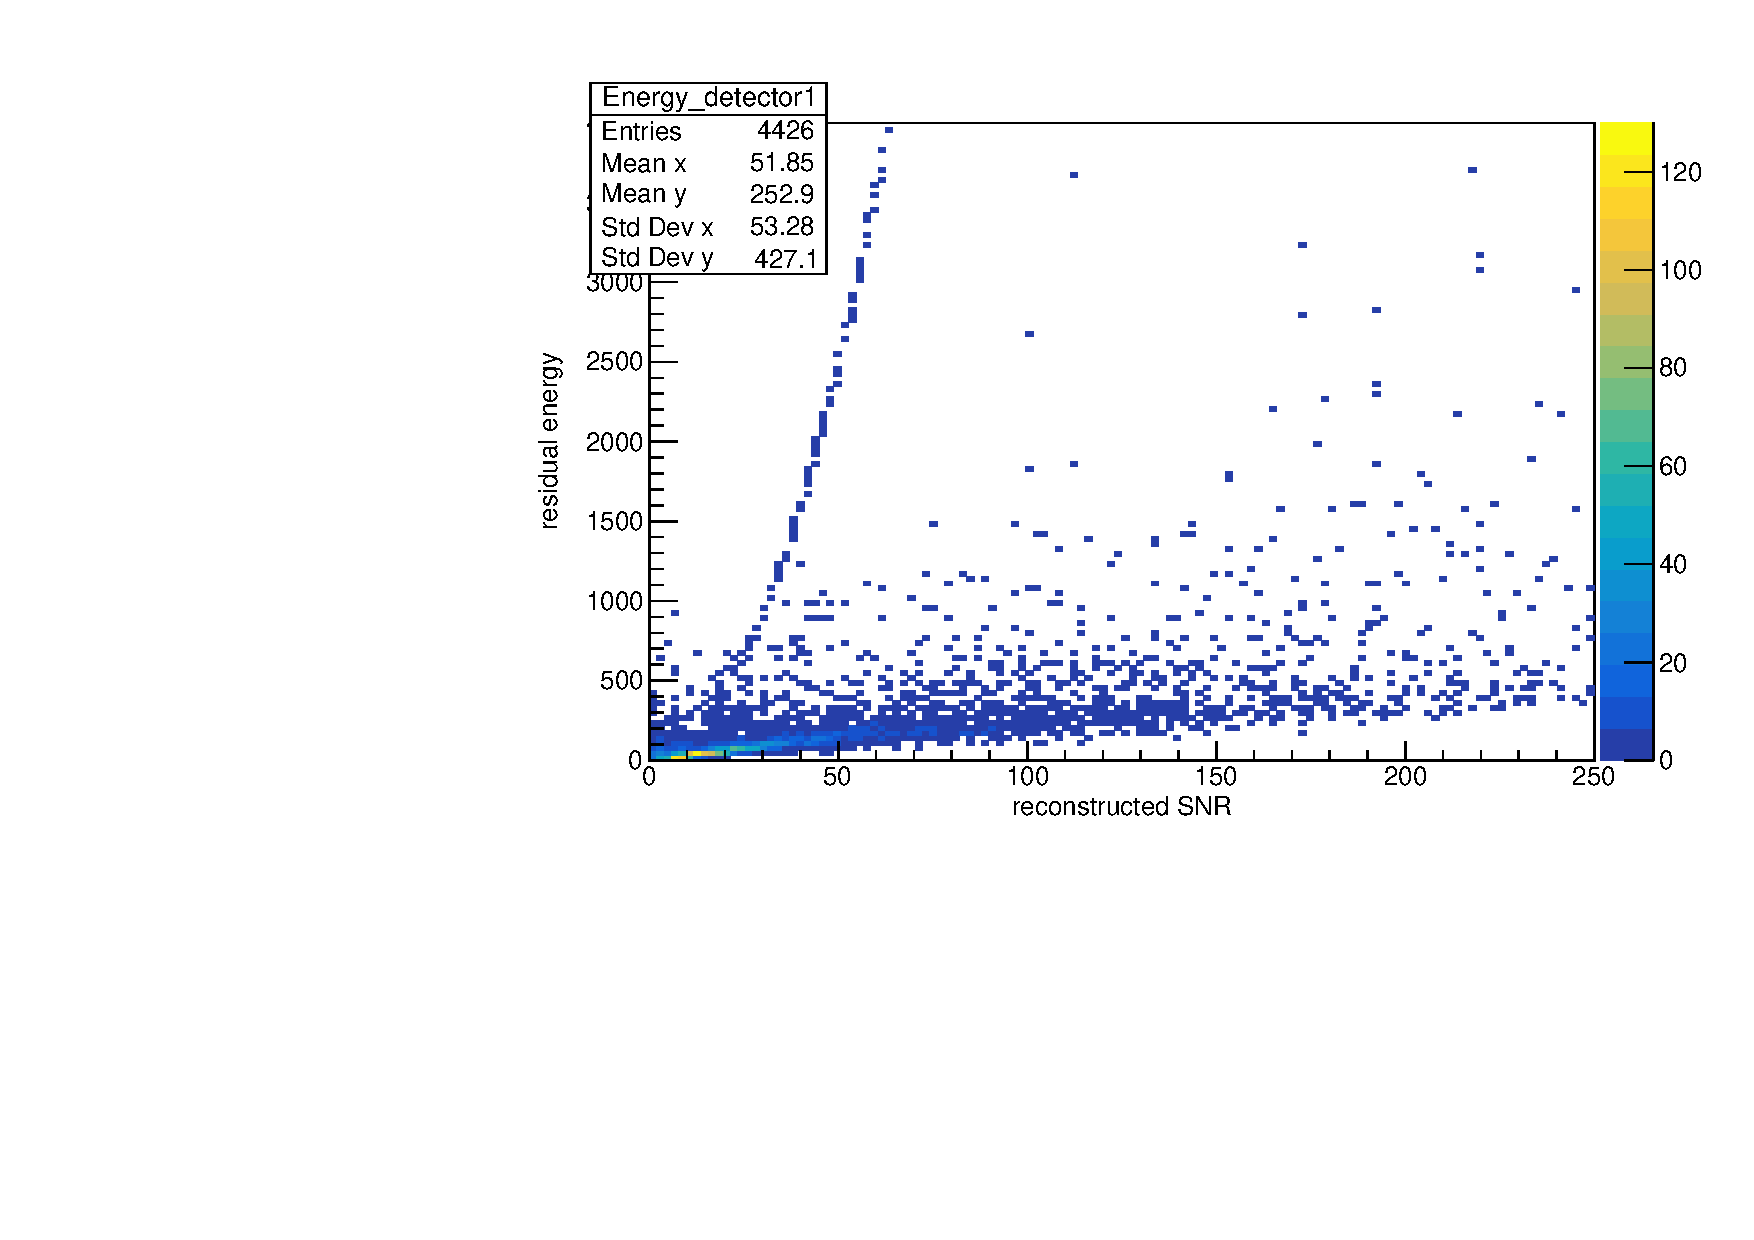
\includegraphics[width=.5\textwidth]{figures/Capitolo_4/EnergyDistributionDetector1APR4_q09.pdf}}
%	\vspace{-5pt}
%	\caption{Energie residue per LIGO-Hanford per le due equazioni di stato}
%	\label{fig:residual_energy}
%	\vspace{-15pt}
%\end{figure}
%\begin{figure}[H]
%	\vspace{-17pt}
%	\centering
%	\subfloat[][\emph{SHT2 per LIGO-Hanford}]
%	{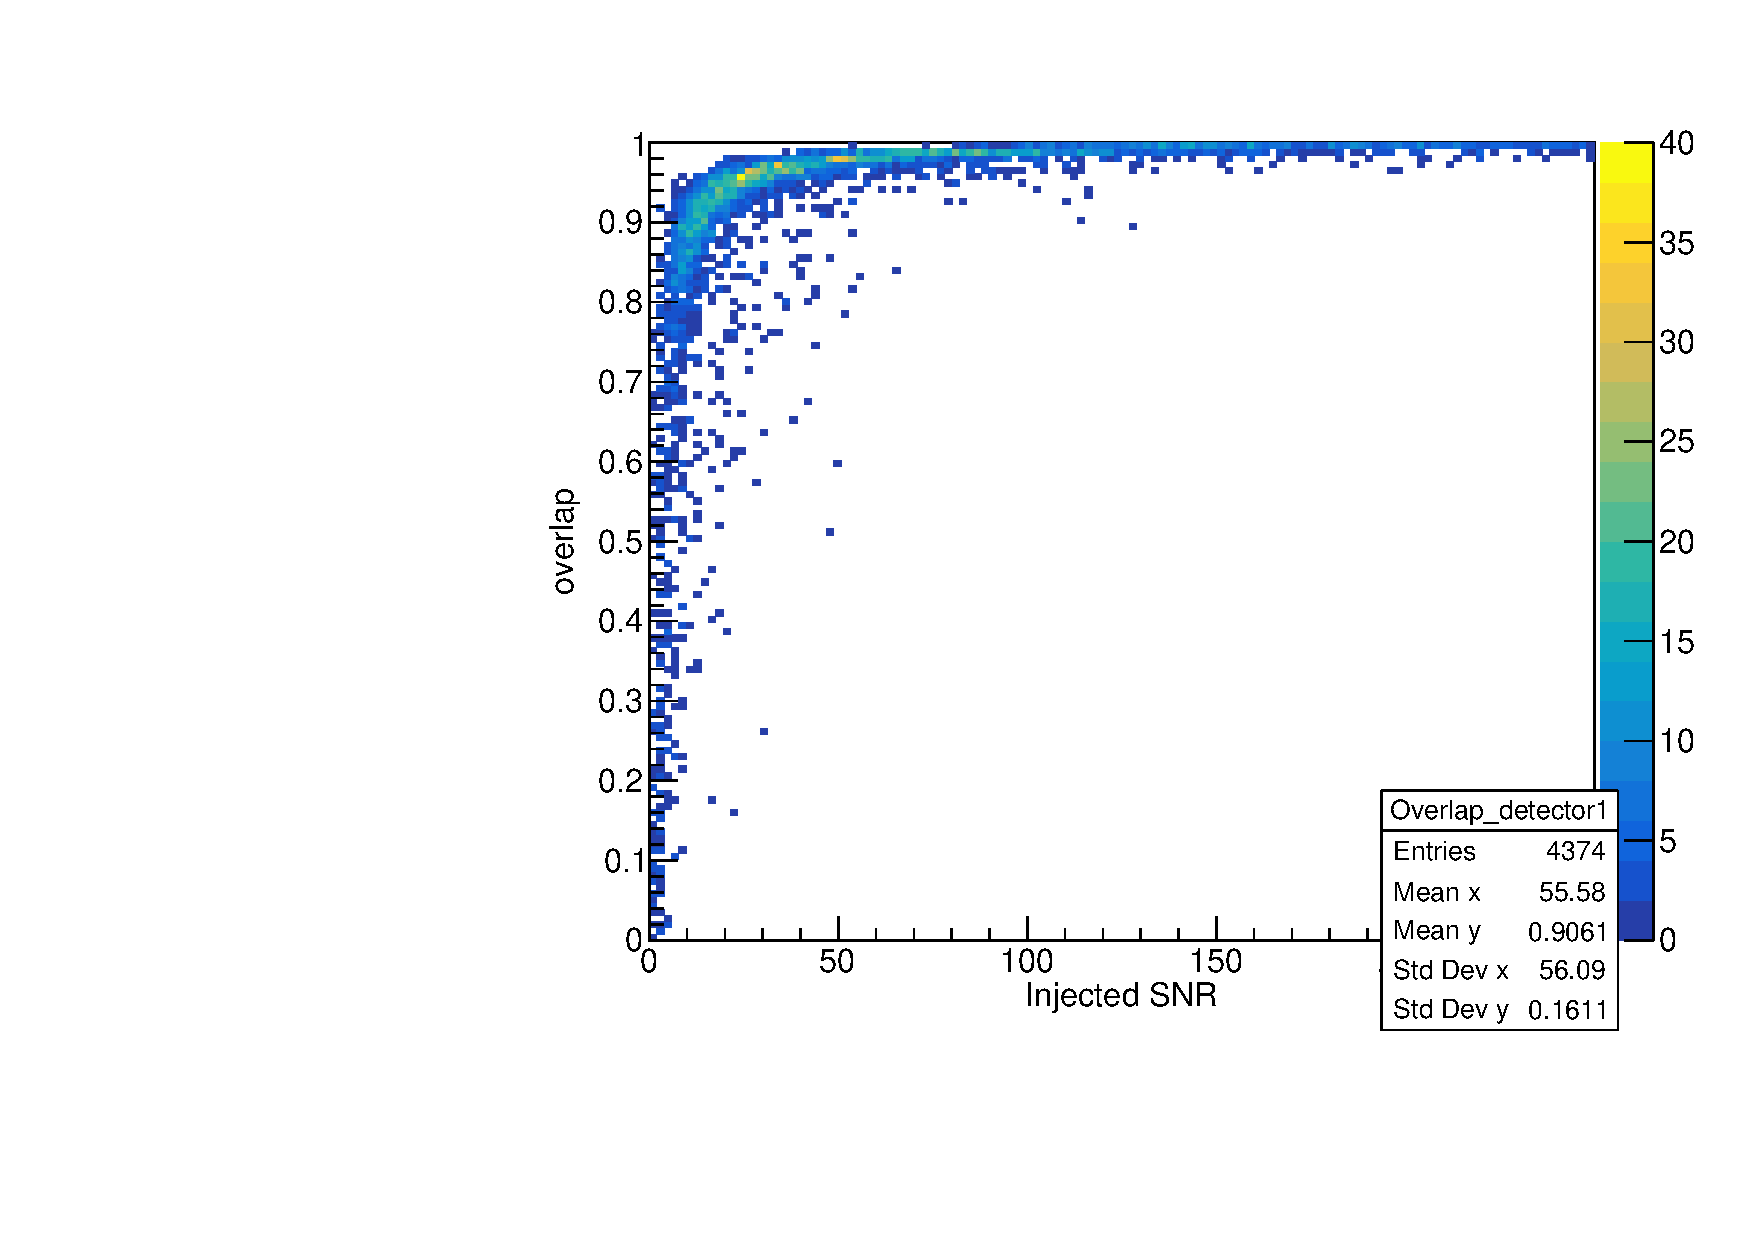
\includegraphics[width=.33\textwidth]{figures/Capitolo_4/OverlapDistributionDetector1SHT2_0spin1.pdf}}
%	\subfloat[][\emph{SHT2 per LIGO-Livingston}]
%	{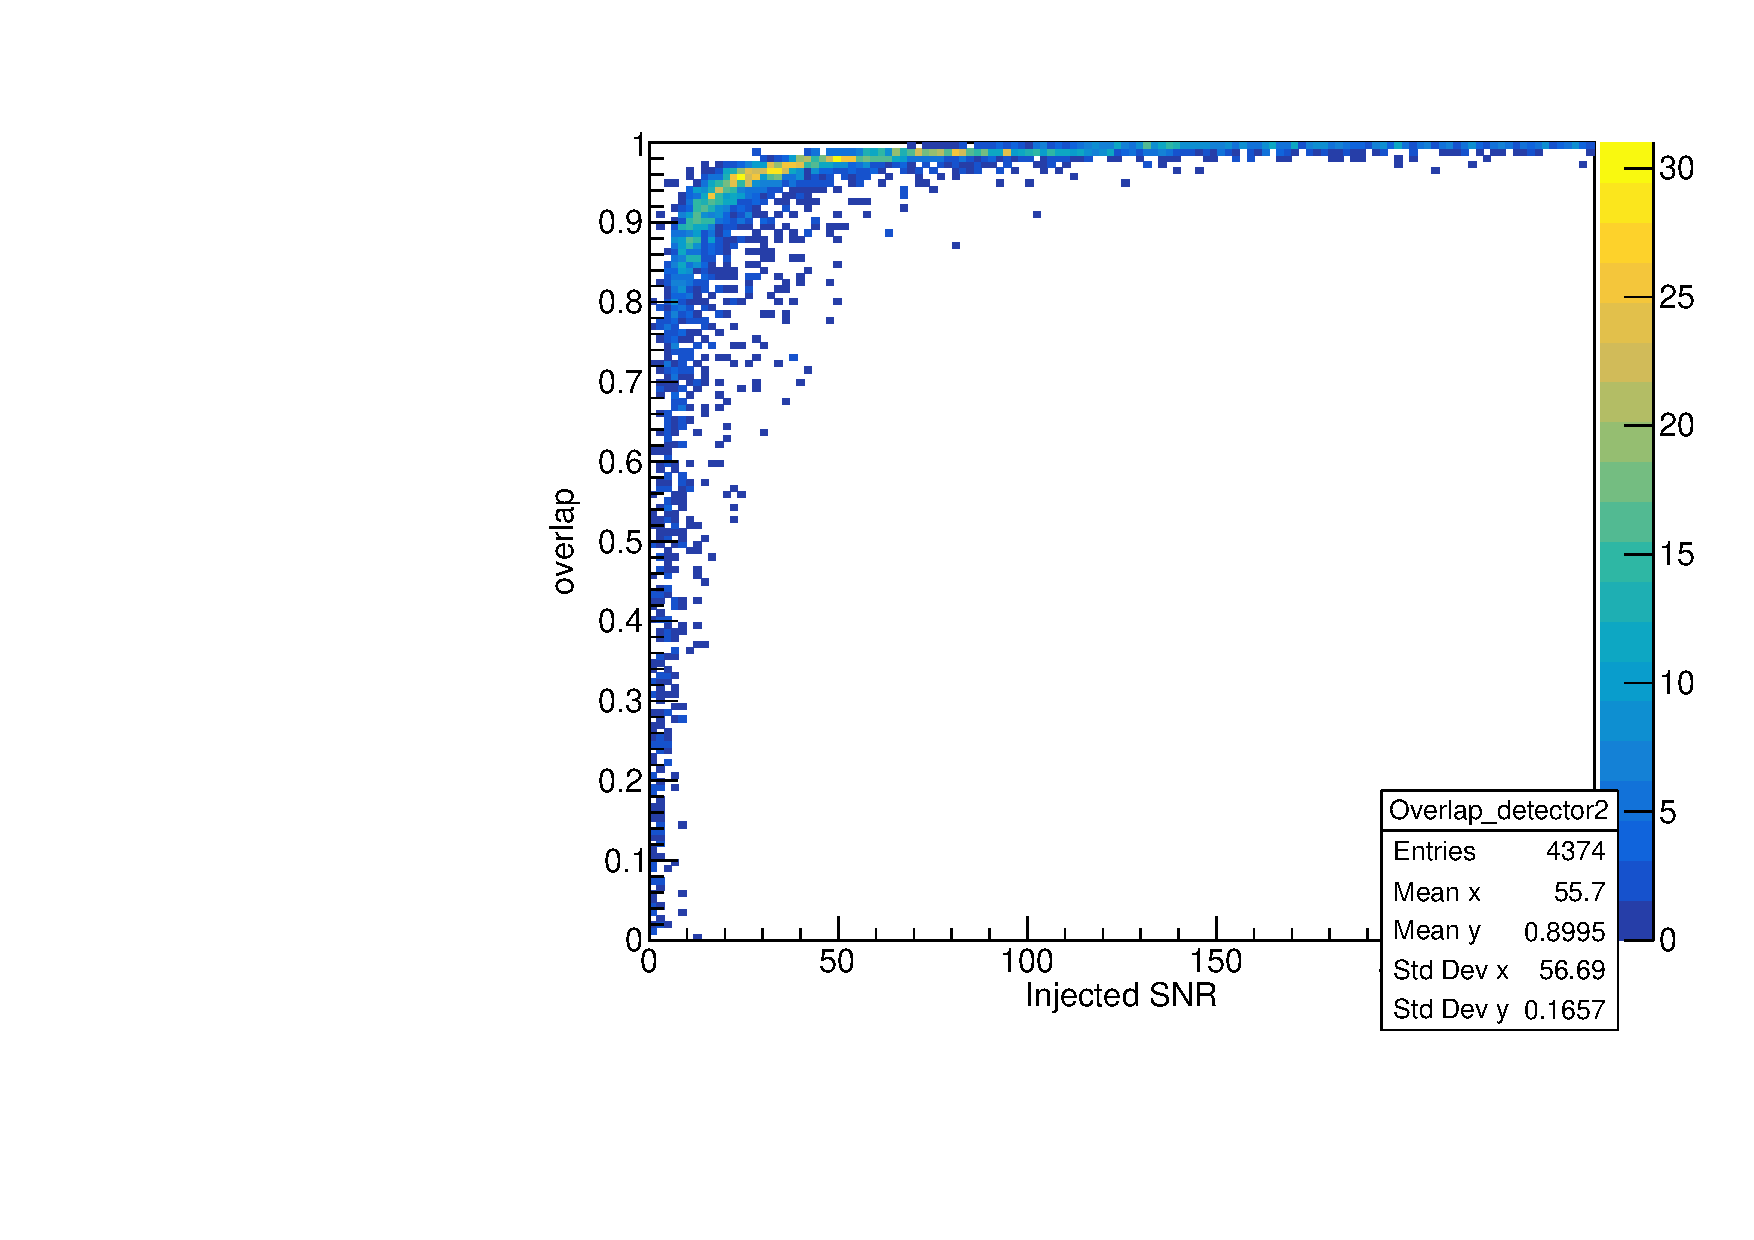
\includegraphics[width=.33\textwidth]{figures/Capitolo_4/OverlapDistributionDetector2SHT2_0spin1.pdf}}
%	\subfloat[][\emph{SHT2 per Virgo}]
%	{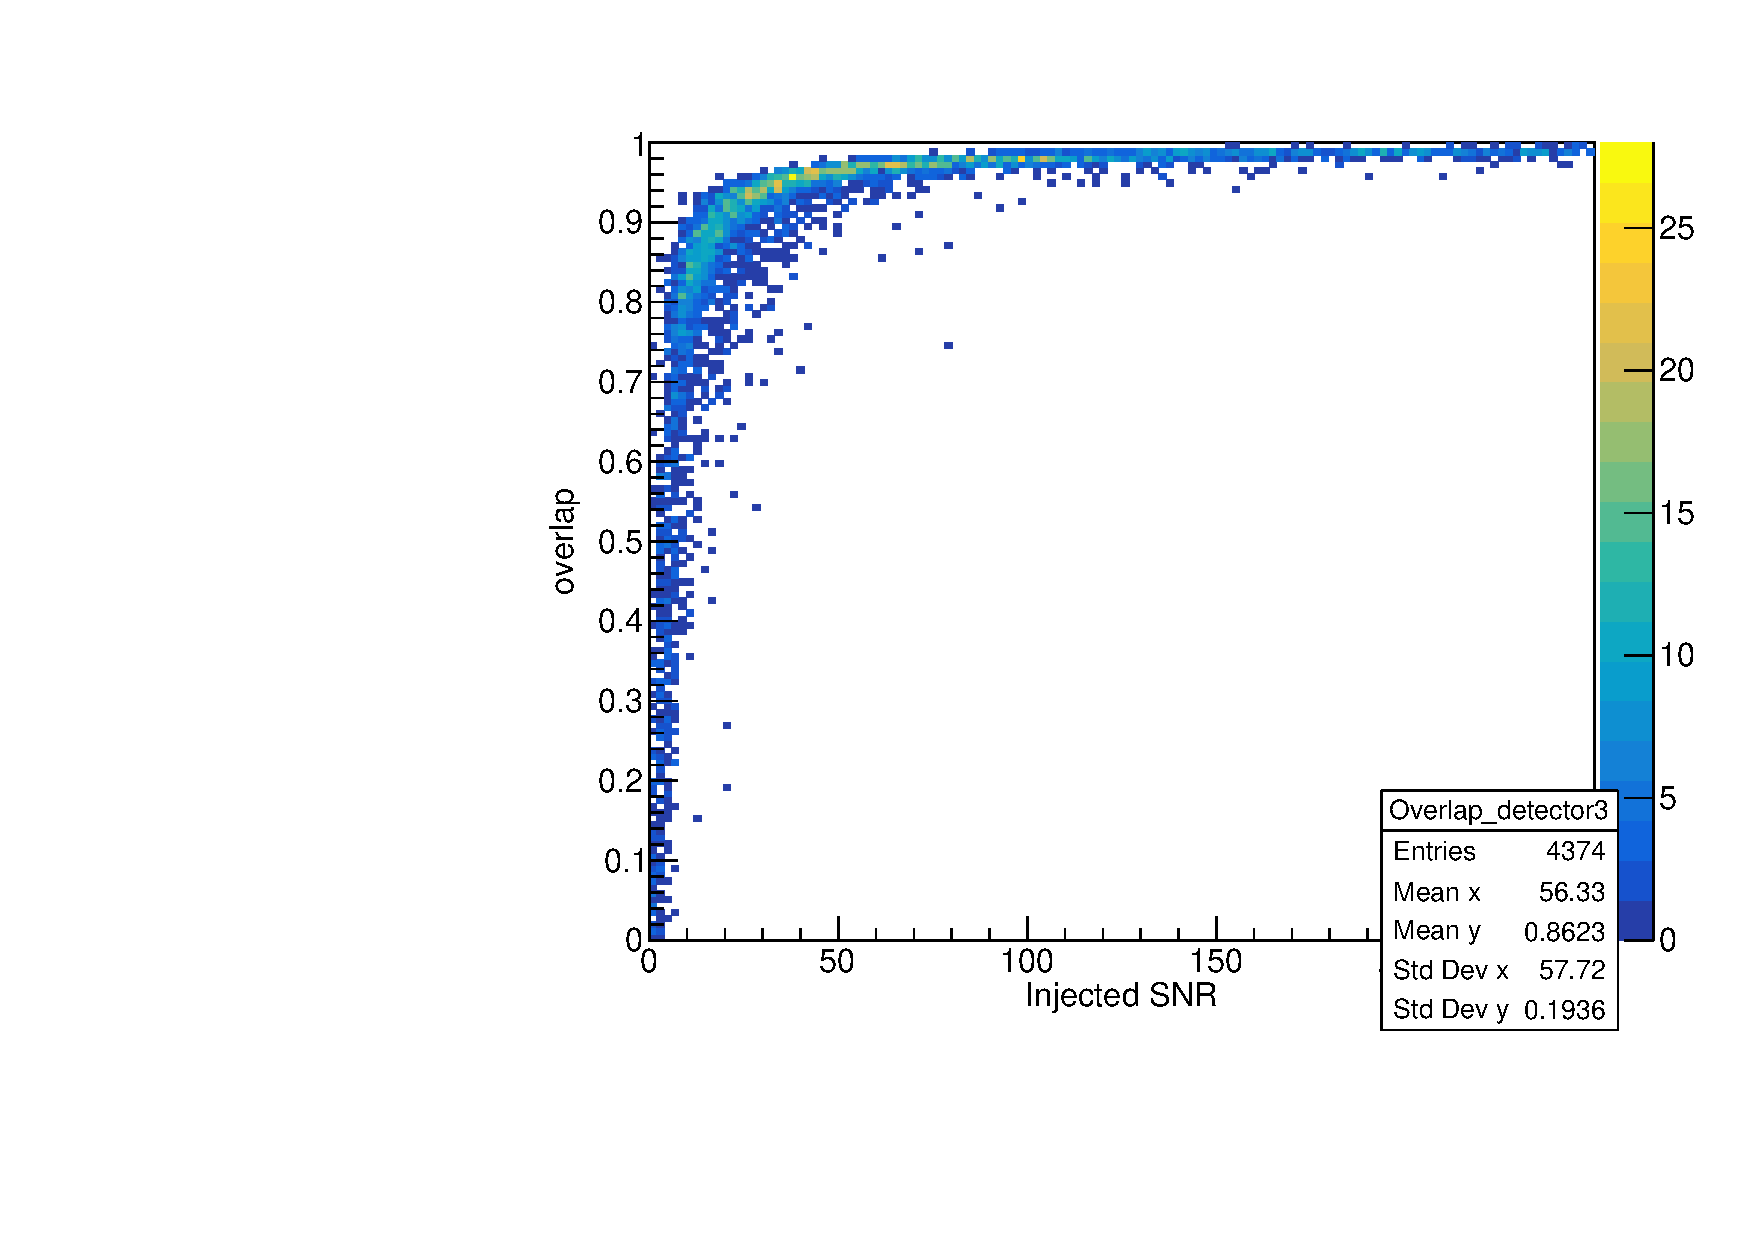
\includegraphics[width=.33\textwidth]{figures/Capitolo_4/OverlapDistributionDetector3SHT2_0spin1.pdf}}\\
%	\vspace{-13pt}
%	\subfloat[][\emph{APR4 per LIGO-Hanford}]
%	{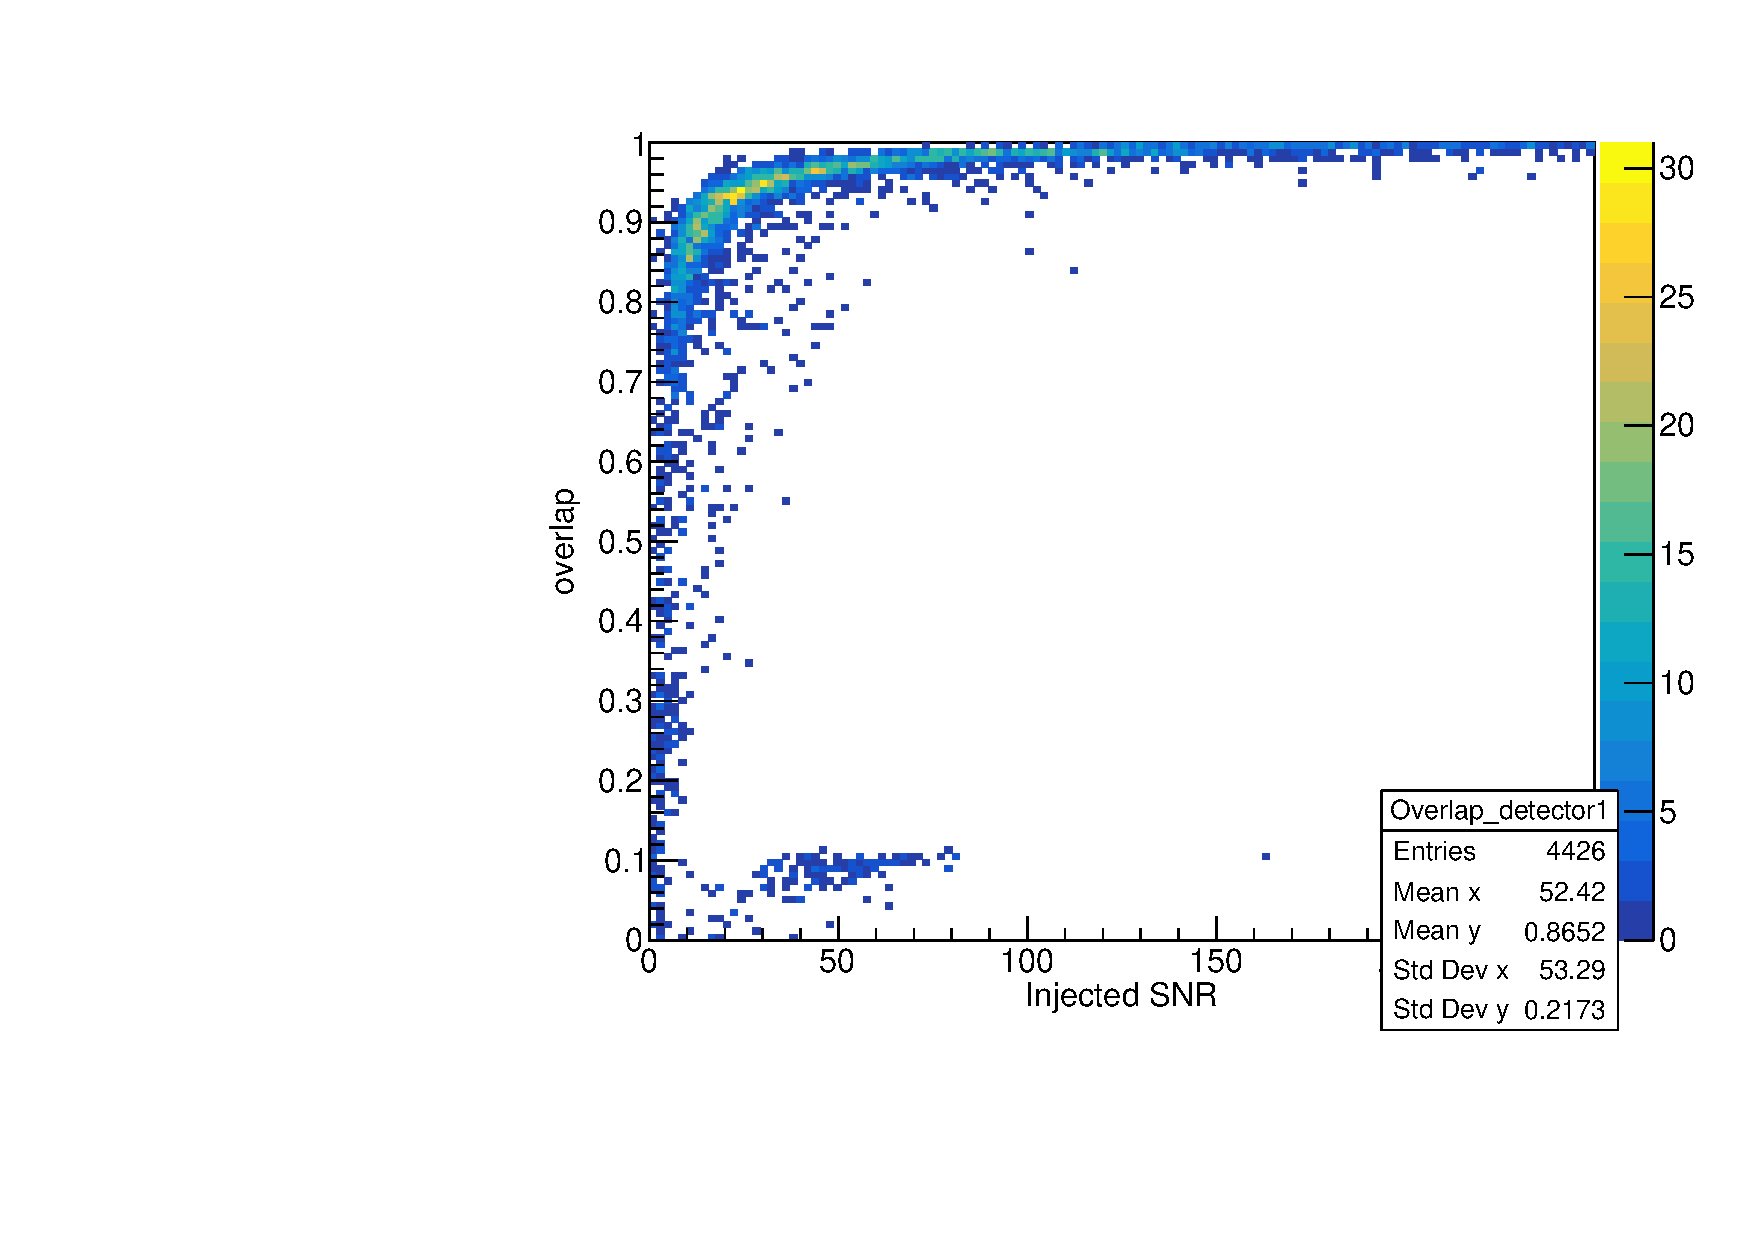
\includegraphics[width=.33\textwidth]{figures/Capitolo_4/OverlapDistributionDetector1APR4_q09.pdf}}
%	\subfloat[][\emph{APR4 per LIGO-Livingston}]
%	{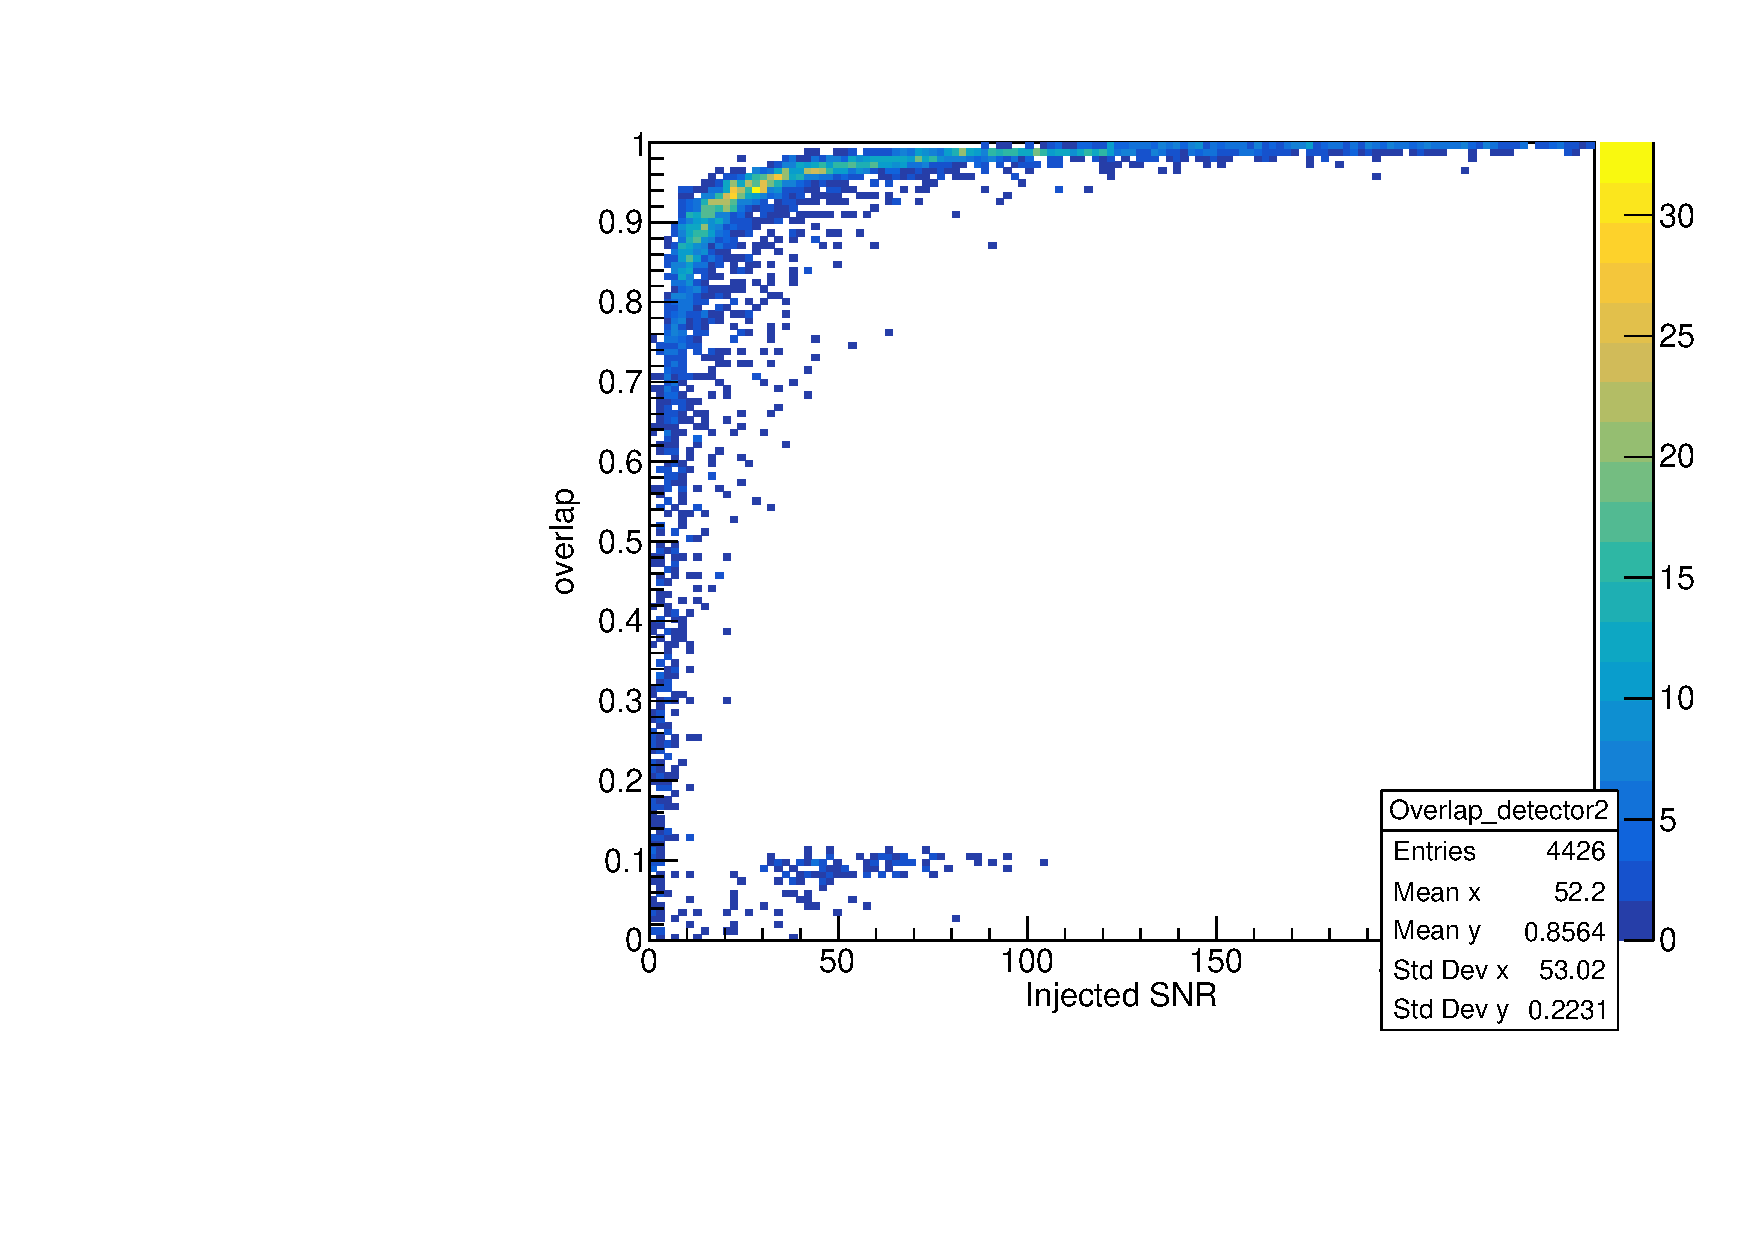
\includegraphics[width=.33\textwidth]{figures/Capitolo_4/OverlapDistributionDetector2APR4_q09.pdf}}
%	\subfloat[][\emph{APR4 per Virgo}]
%	{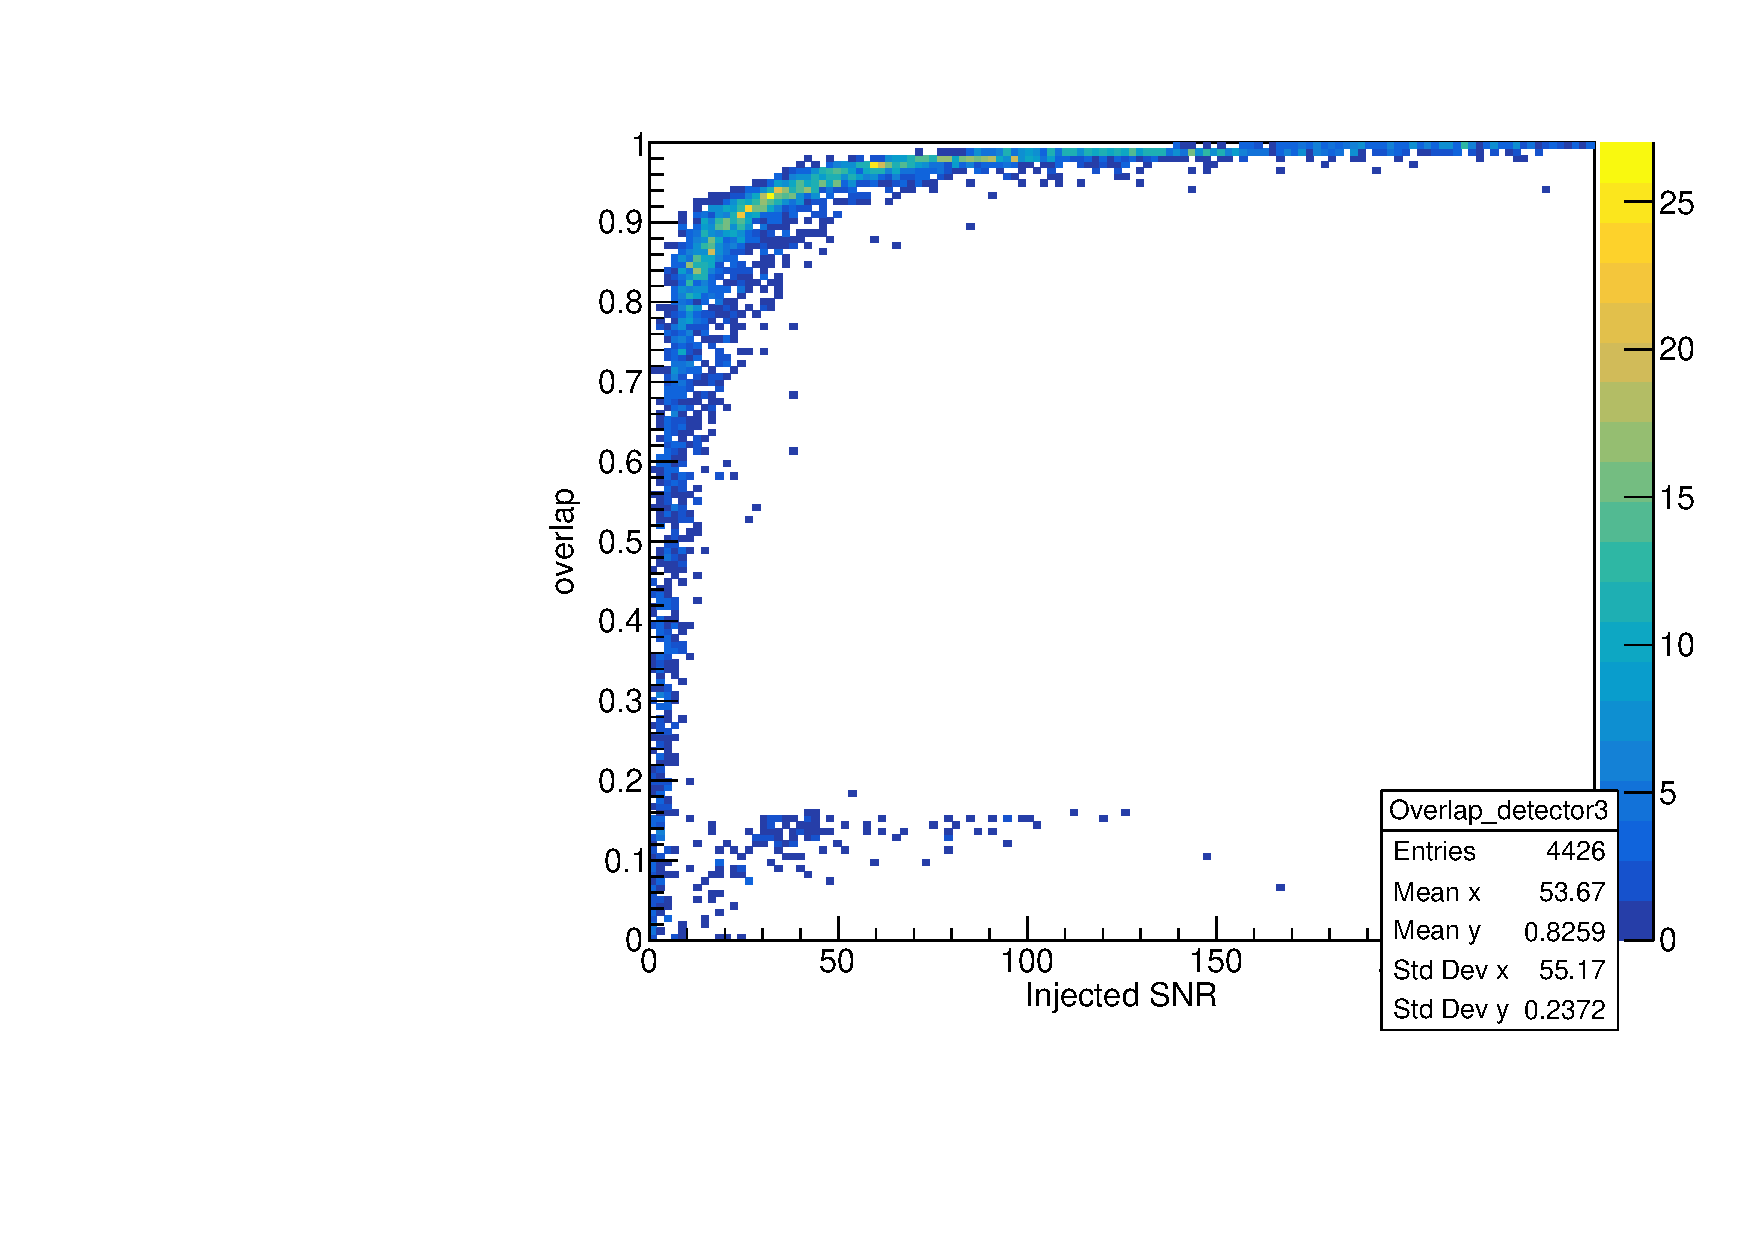
\includegraphics[width=.33\textwidth]{figures/Capitolo_4/OverlapDistributionDetector3APR4_q09.pdf}}
%	\vspace{-5pt}
%	\caption{Overlap per le due equazioni di stato}
%	\label{fig:Overlap_SHT2_APR4}
%	\vspace{-15pt}
%\end{figure}
\begin{figure}[ht]
	\vspace{-20pt}
	\centering
	\subfloat[][\emph{SHT2.0}]
	{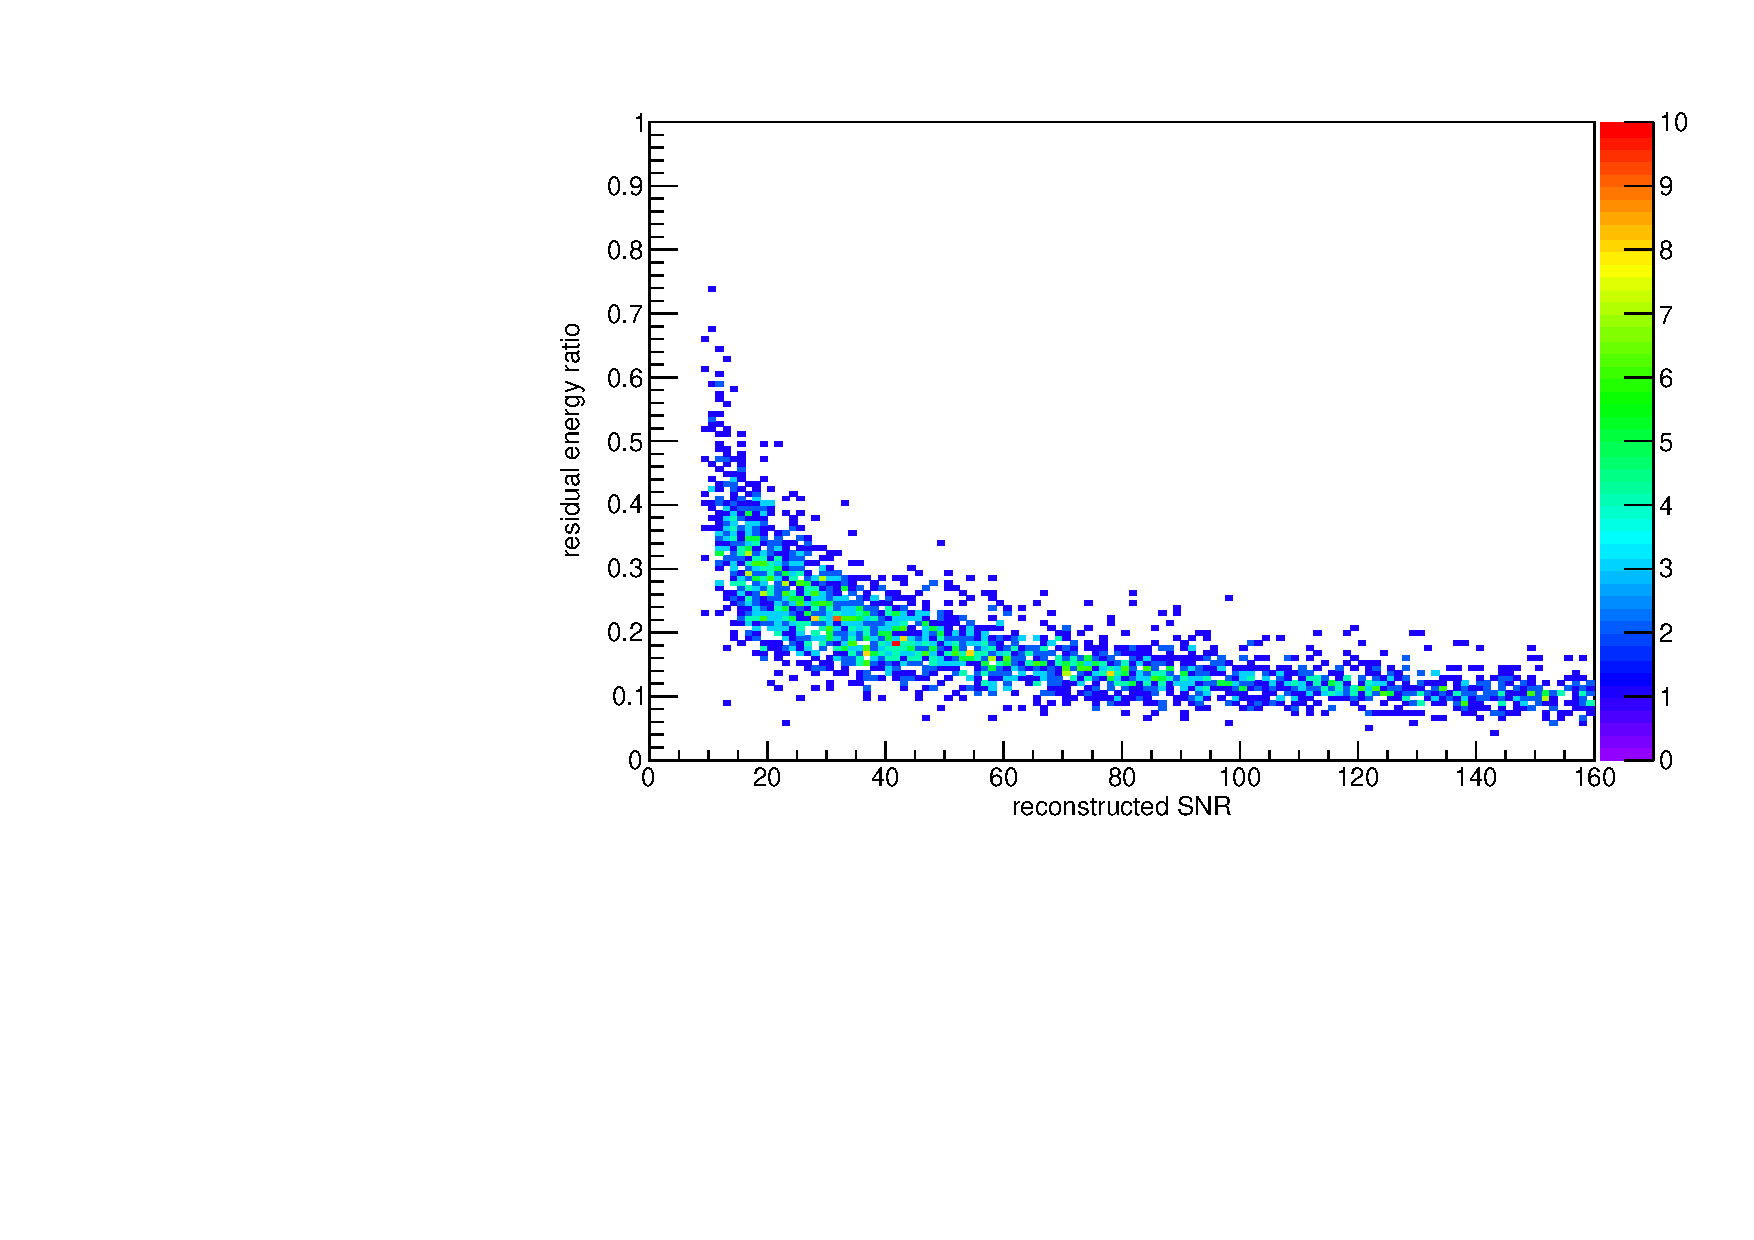
\includegraphics[width=.3333333333333\textwidth]{figures/Capitolo_4/report/RatioResidualEnergyDistributionDetector1SHT2_0spin1.pdf}}
	\subfloat[][\emph{SHT2.2}]
	{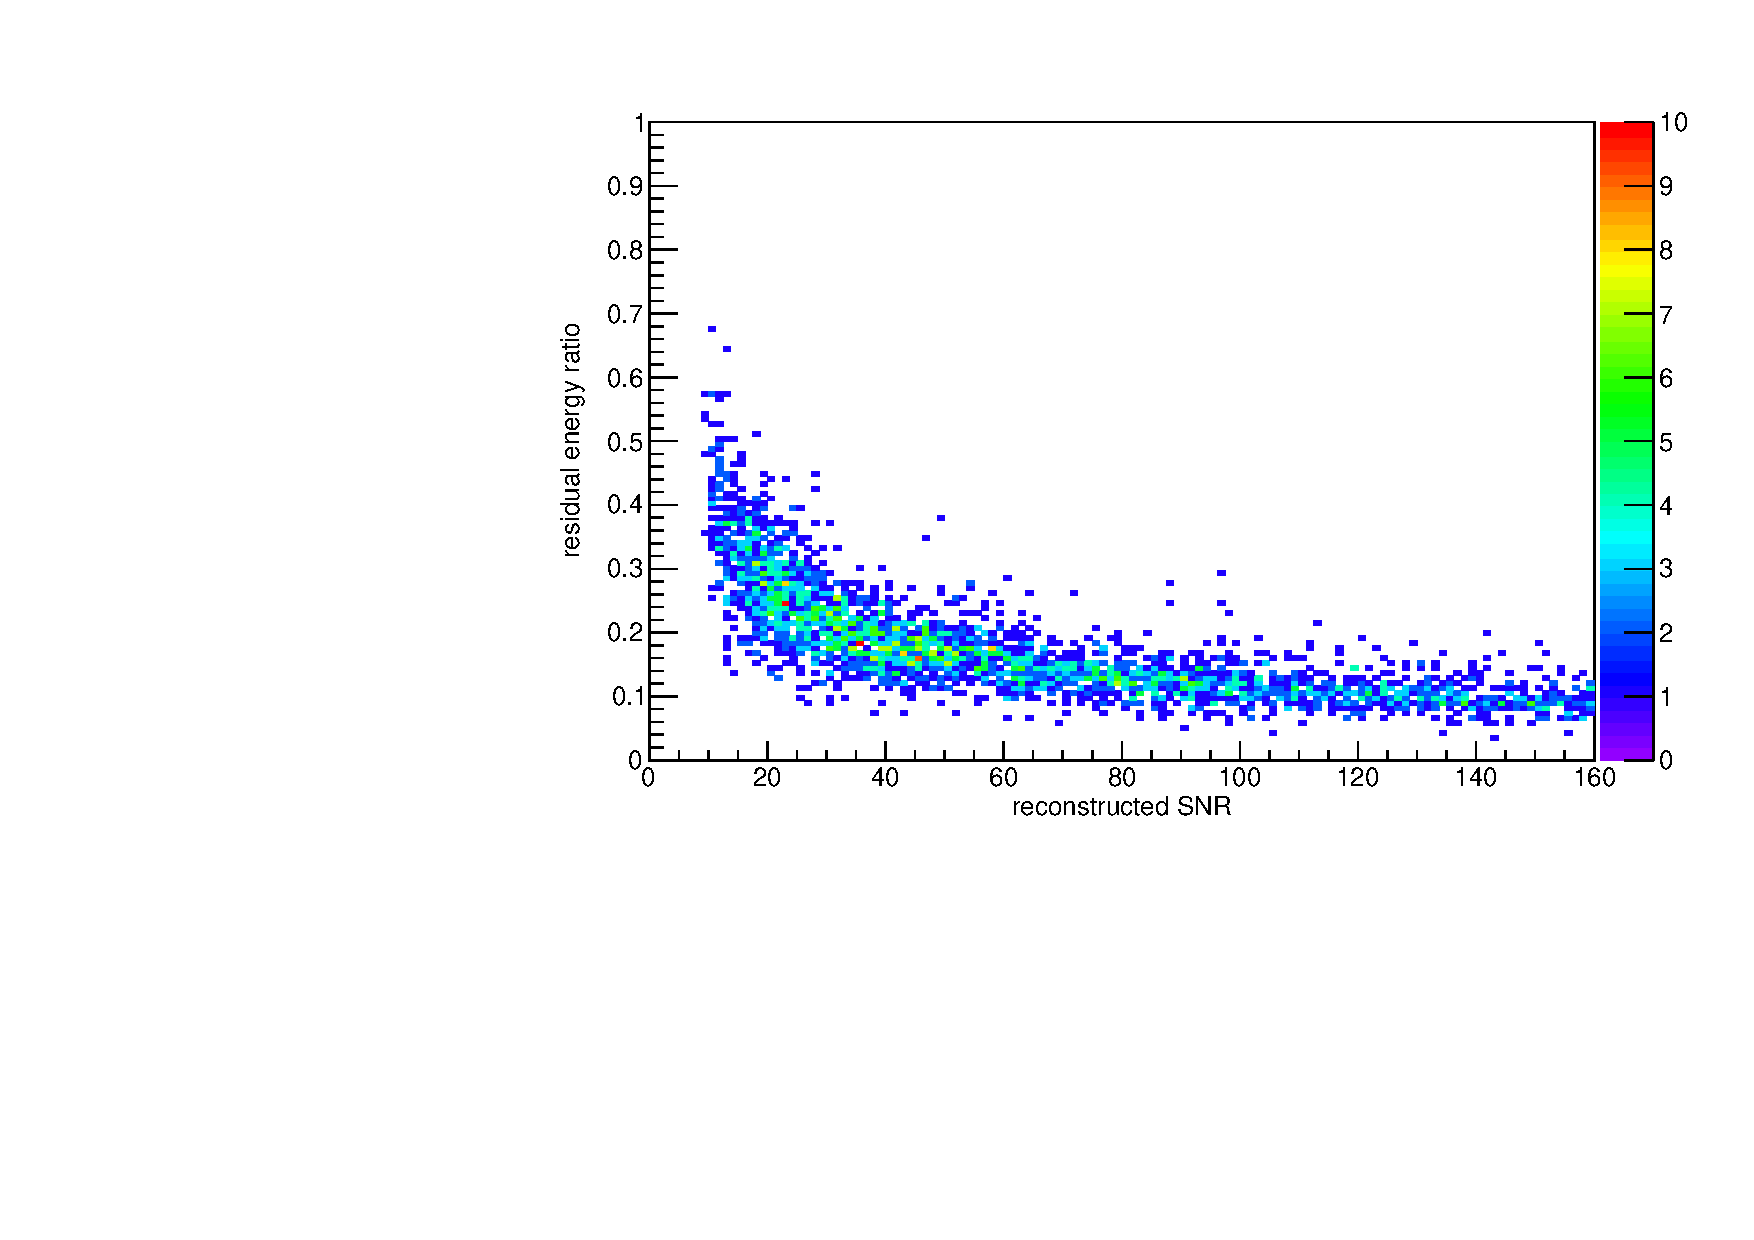
\includegraphics[width=.3333333333333\textwidth]{figures/Capitolo_4/report/RatioResidualEnergyDistributionDetector1SHT2_2spin1.pdf}}
	\subfloat[][\emph{APR4}]
	{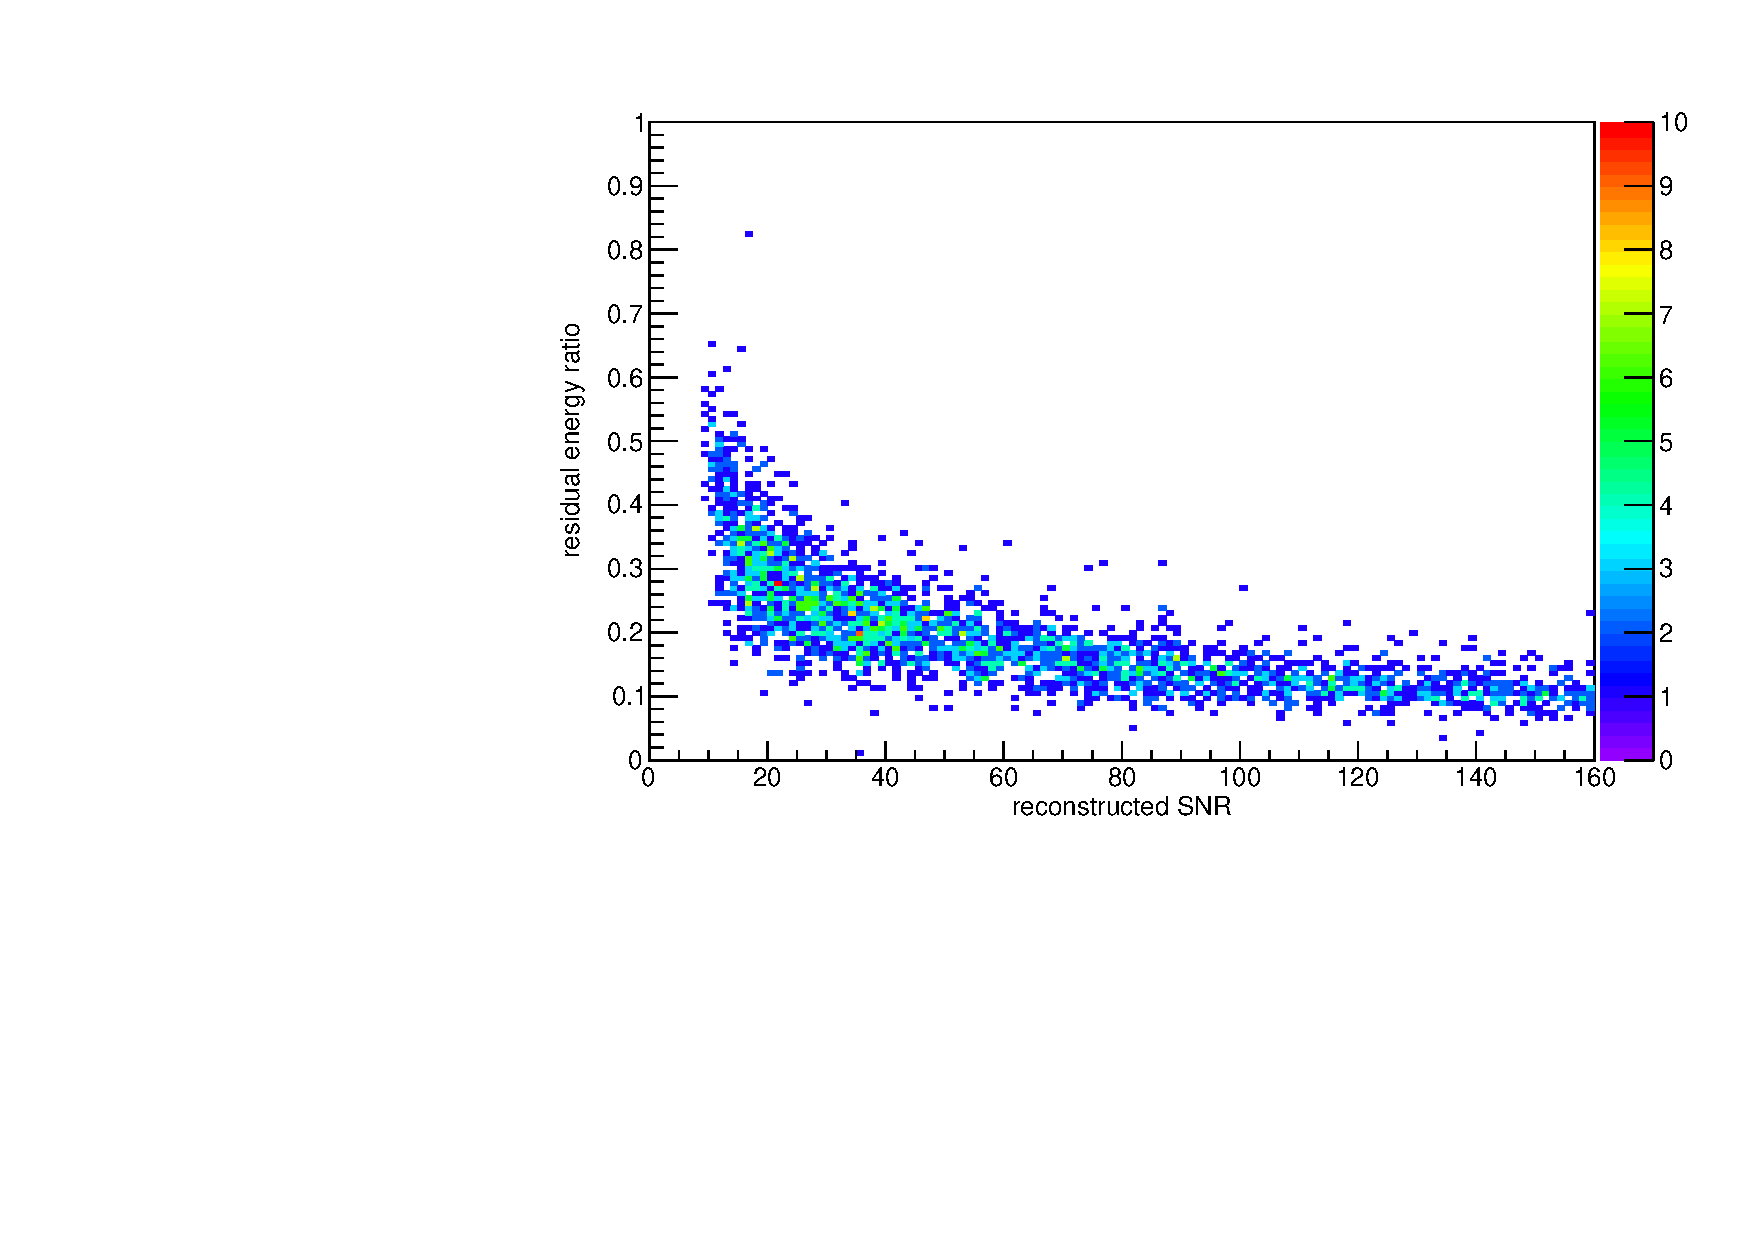
\includegraphics[width=.3333333333333\textwidth]{figures/Capitolo_4/report/RatioResidualEnergyDistributionDetector1APR4_q09.pdf}}
	\vspace{-8pt}
	\caption{Rapporto dell'energia residua rispetto all'energia totale dell'evento misurata da LIGO-Hanford}
	\label{fig:residual_energy}
	\vspace{-15pt}
\end{figure}
\begin{figure}[ht]
	\vspace{-17pt}
	\centering
	\subfloat[][\emph{SHT2.0 per LIGO-Hanford}]
	{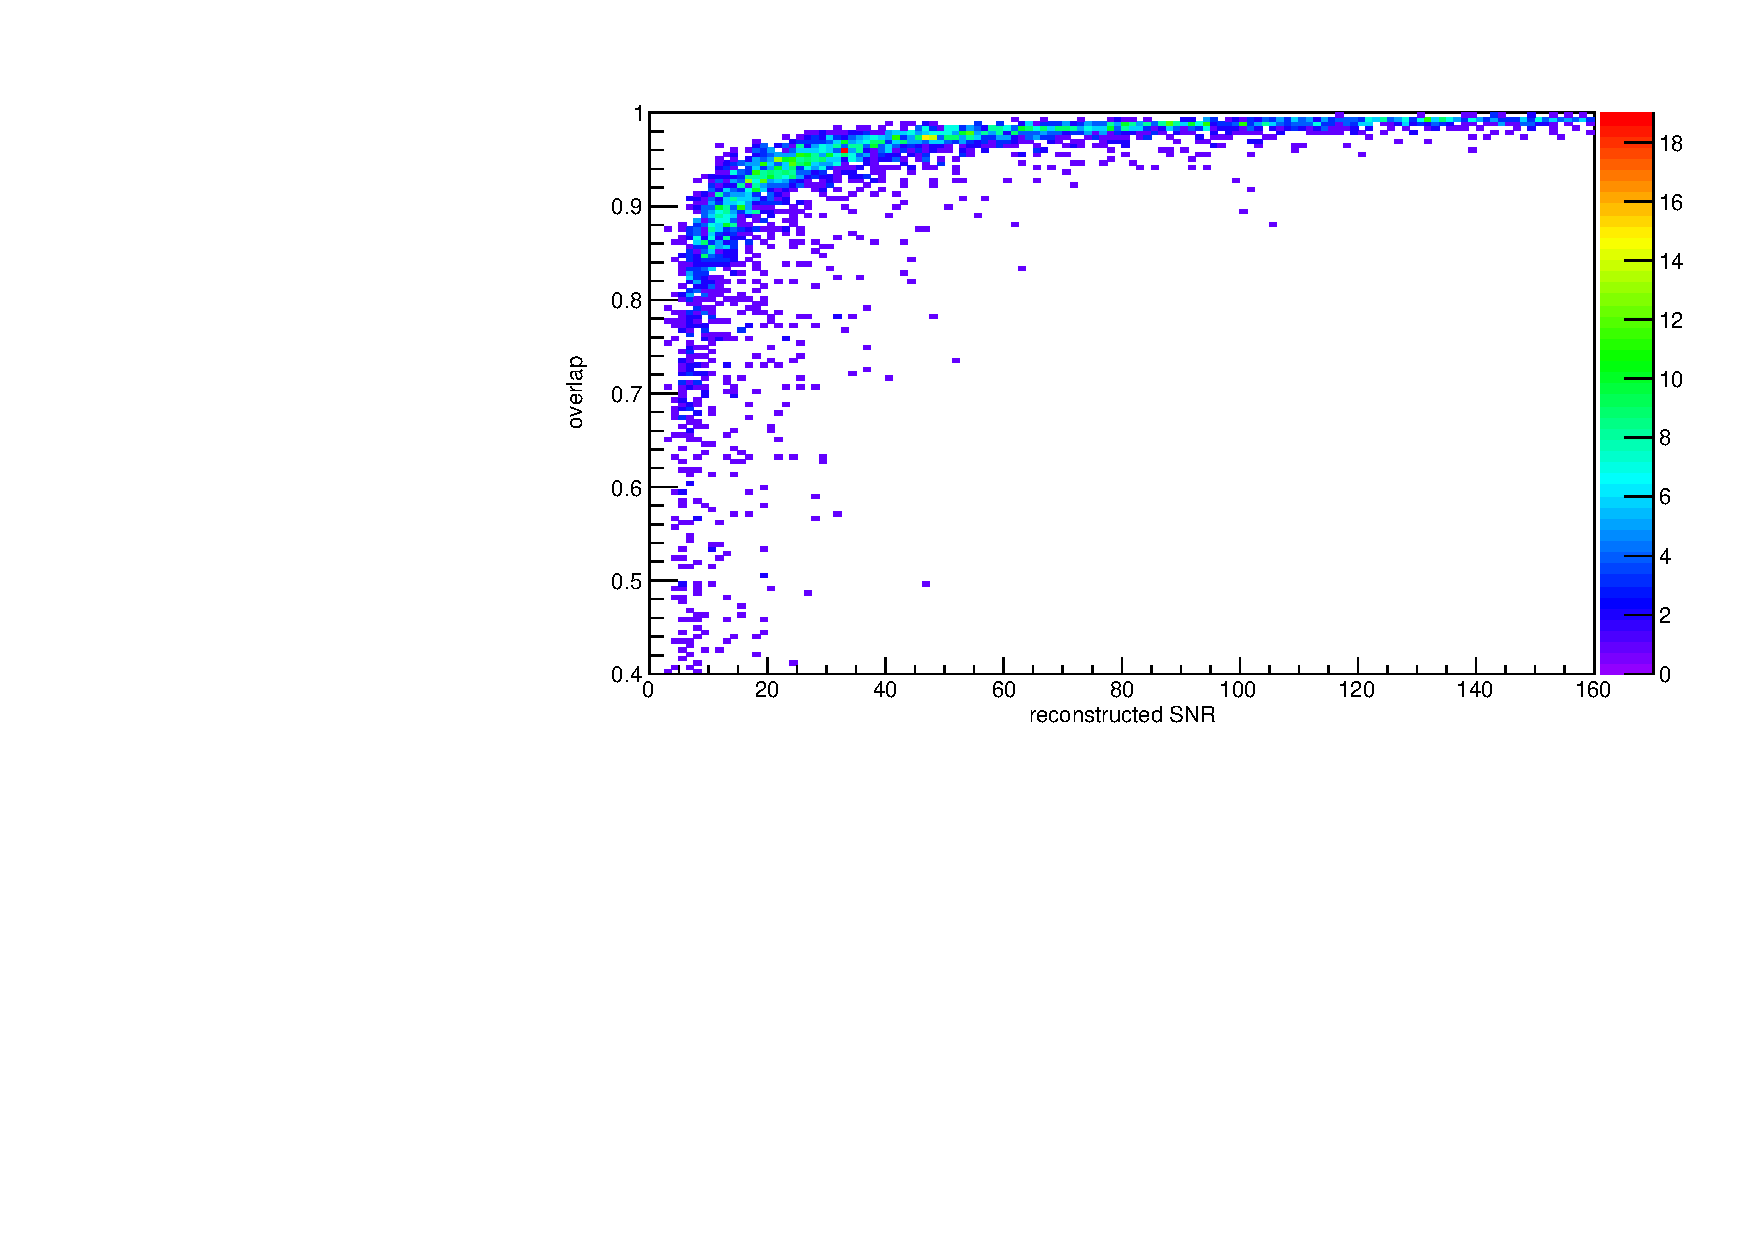
\includegraphics[width=.33\textwidth]{figures/Capitolo_4/report/OverlapDistributionDetector1SHT2_0spin1.pdf}}
	\subfloat[][\emph{SHT2.0 per LIGO-Livingston}]
	{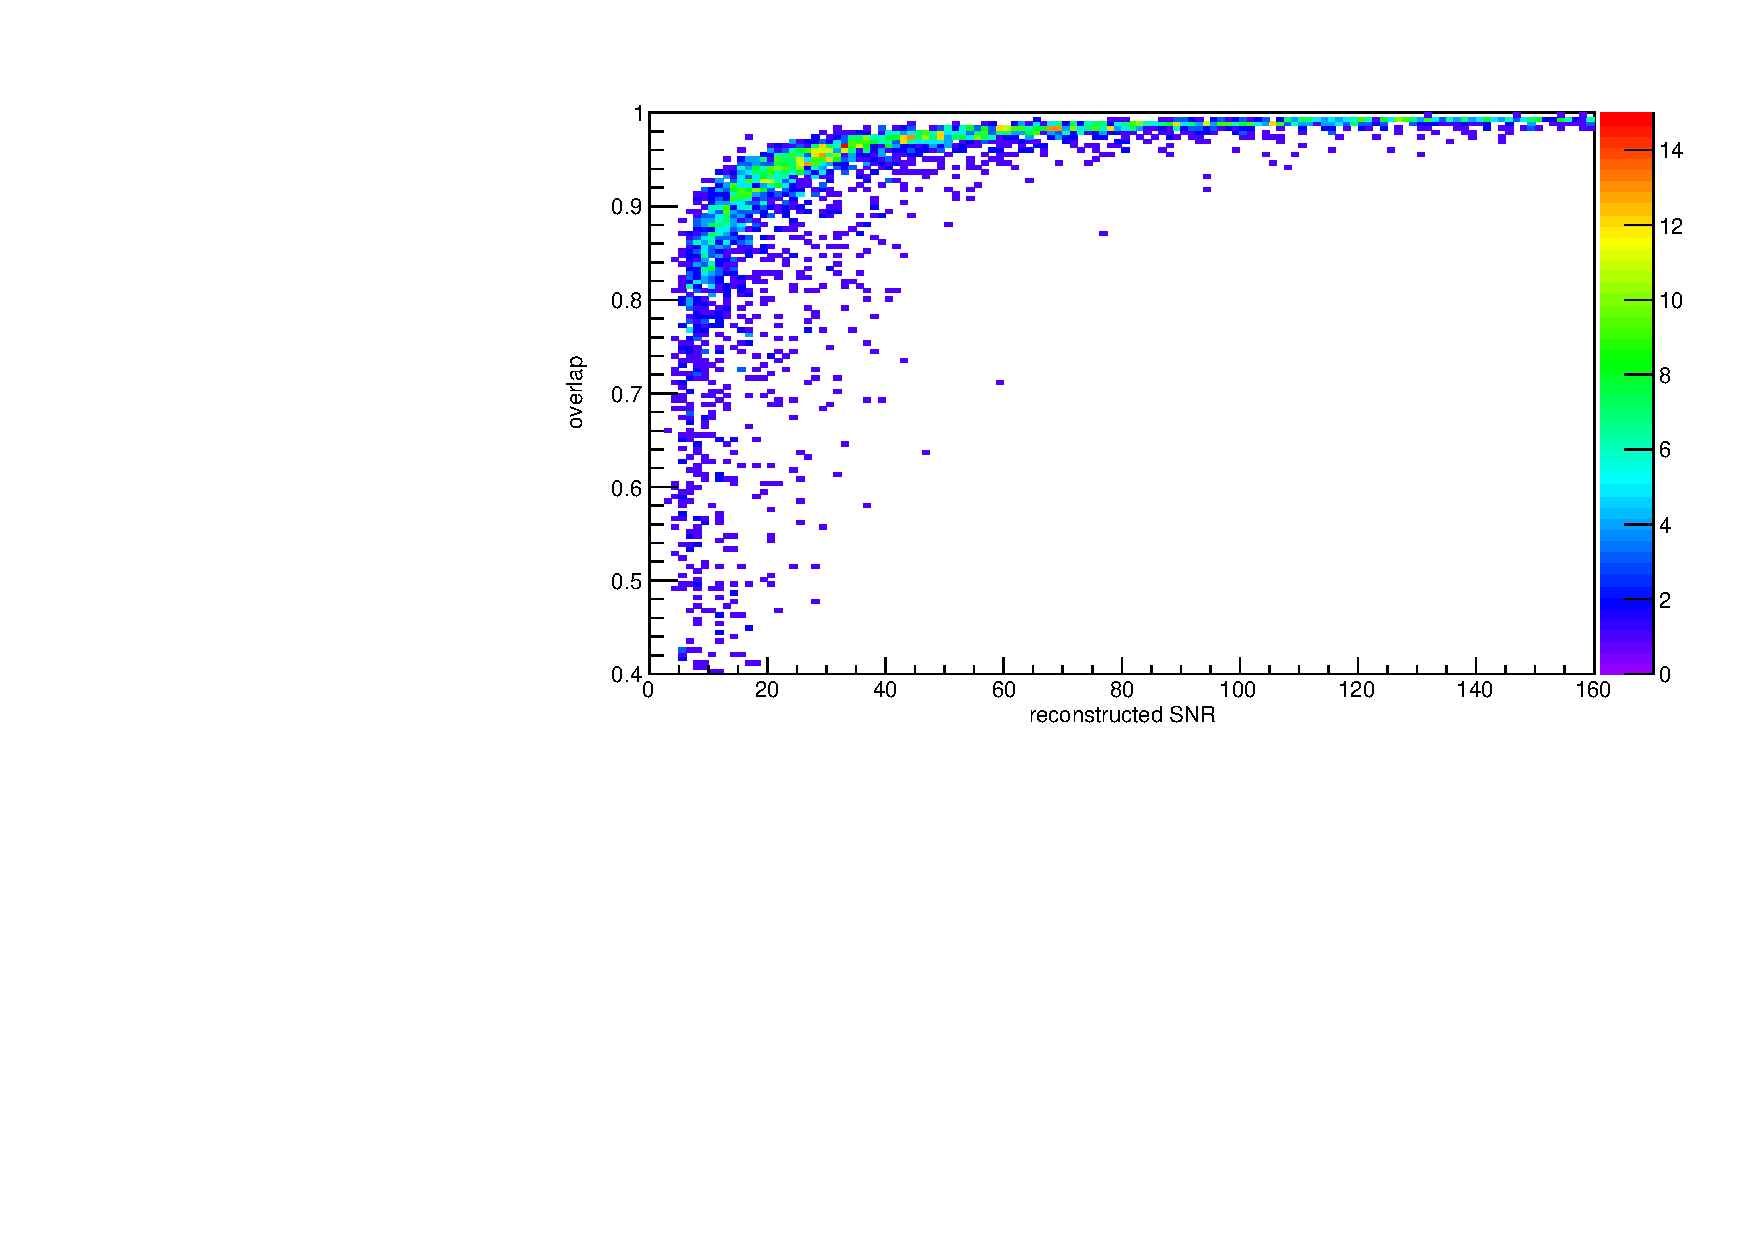
\includegraphics[width=.33\textwidth]{figures/Capitolo_4/report/OverlapDistributionDetector2SHT2_0spin1.pdf}}
	\subfloat[][\emph{SHT2.0 per Virgo}]
	{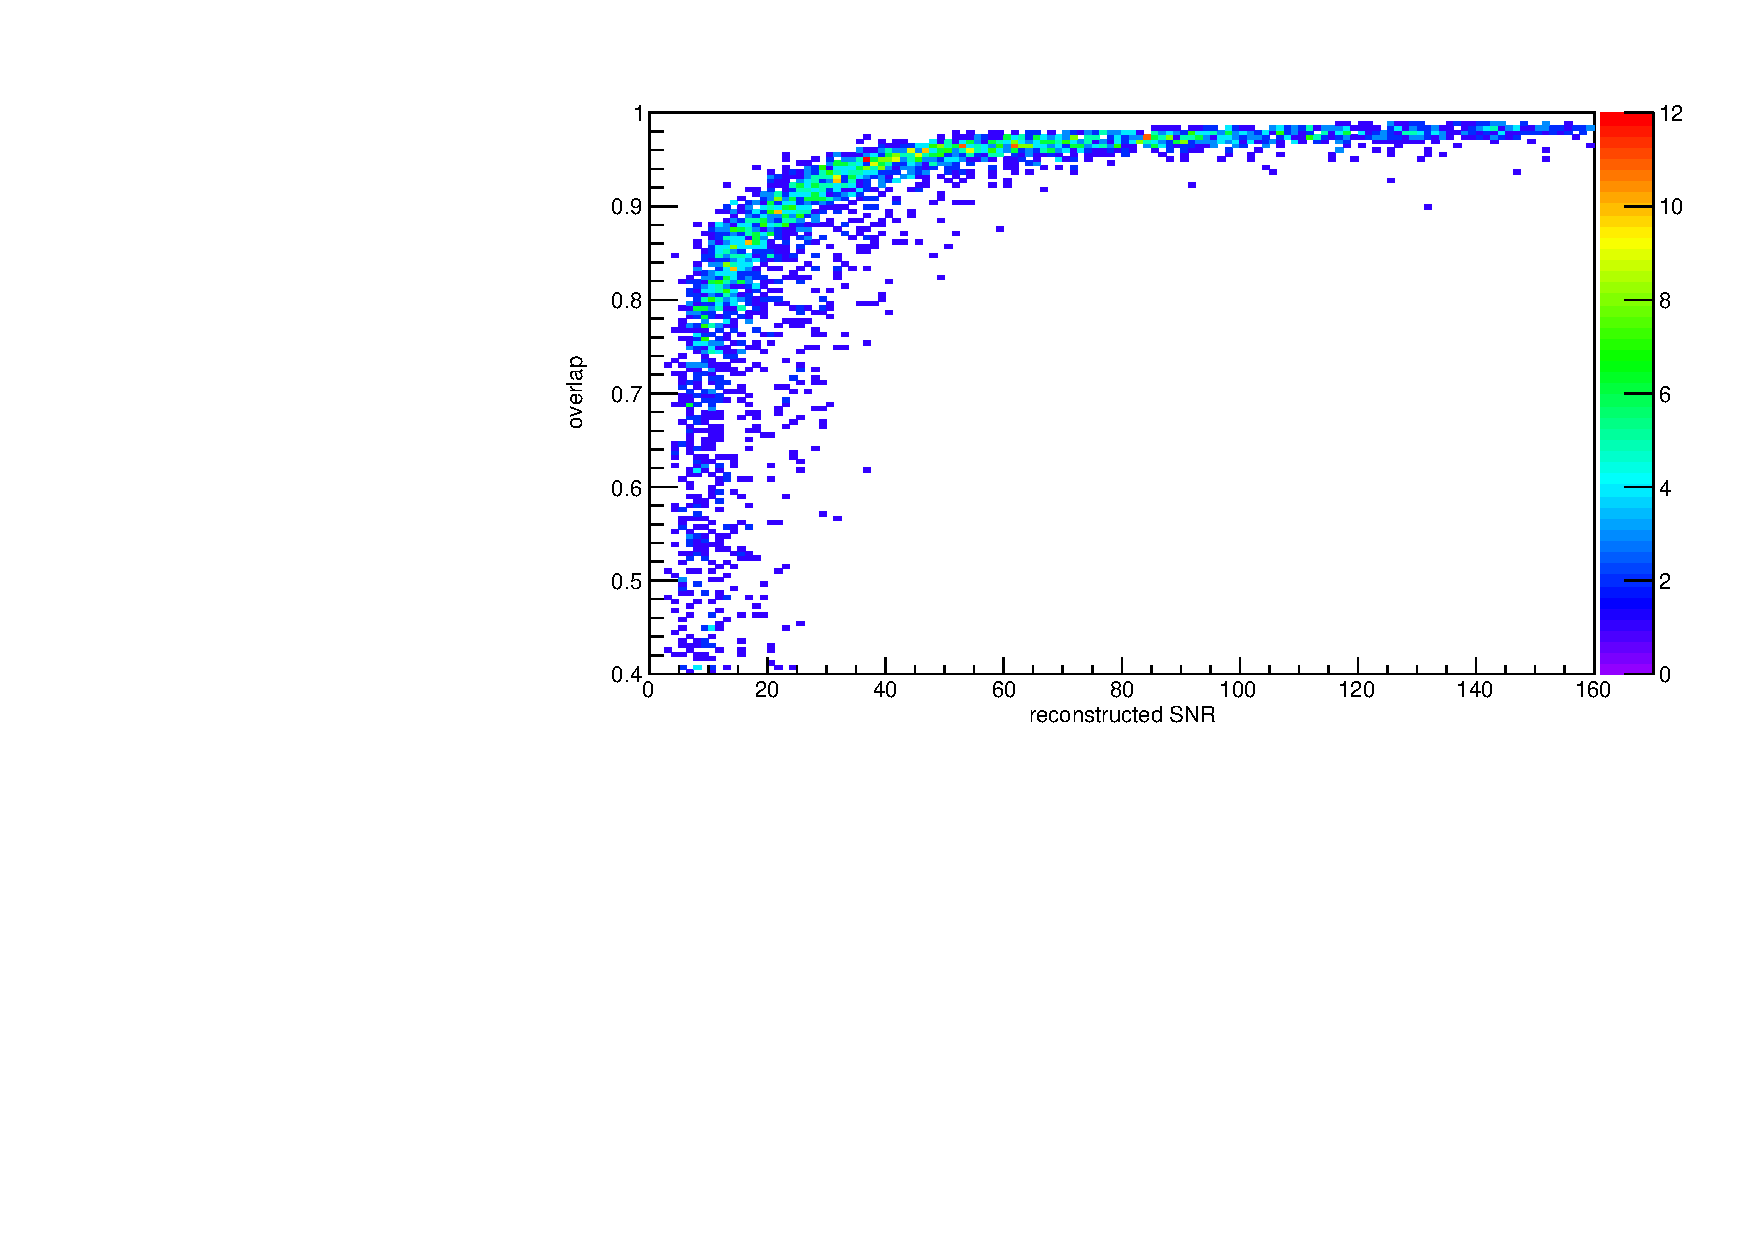
\includegraphics[width=.33\textwidth]{figures/Capitolo_4/report/OverlapDistributionDetector3SHT2_0spin1.pdf}}\\
	\vspace{-13pt}
	\subfloat[][\emph{SHT2.2 per LIGO-Hanford}]
	{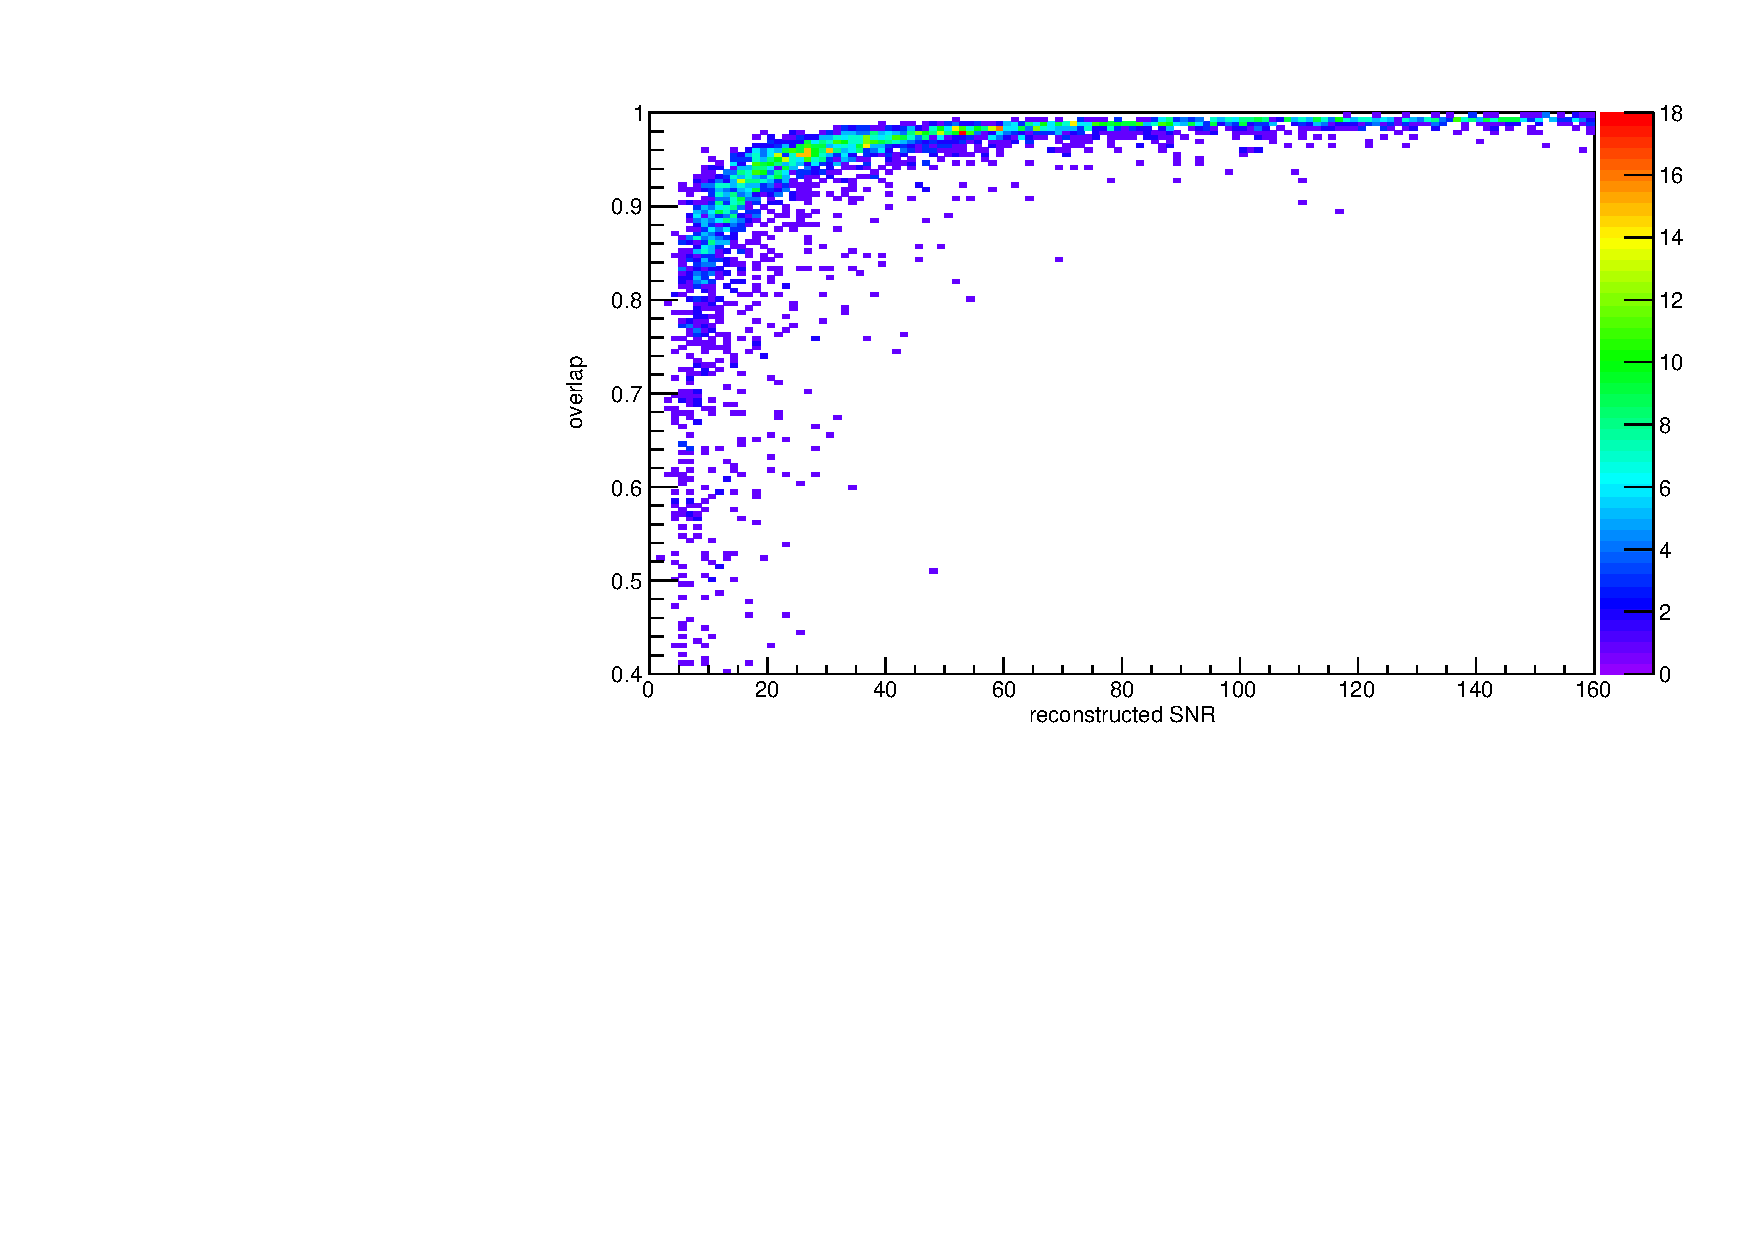
\includegraphics[width=.33\textwidth]{figures/Capitolo_4/report/OverlapDistributionDetector1SHT2_2spin1.pdf}}
	\subfloat[][\emph{SHT2.2 per LIGO-Livingston}]
	{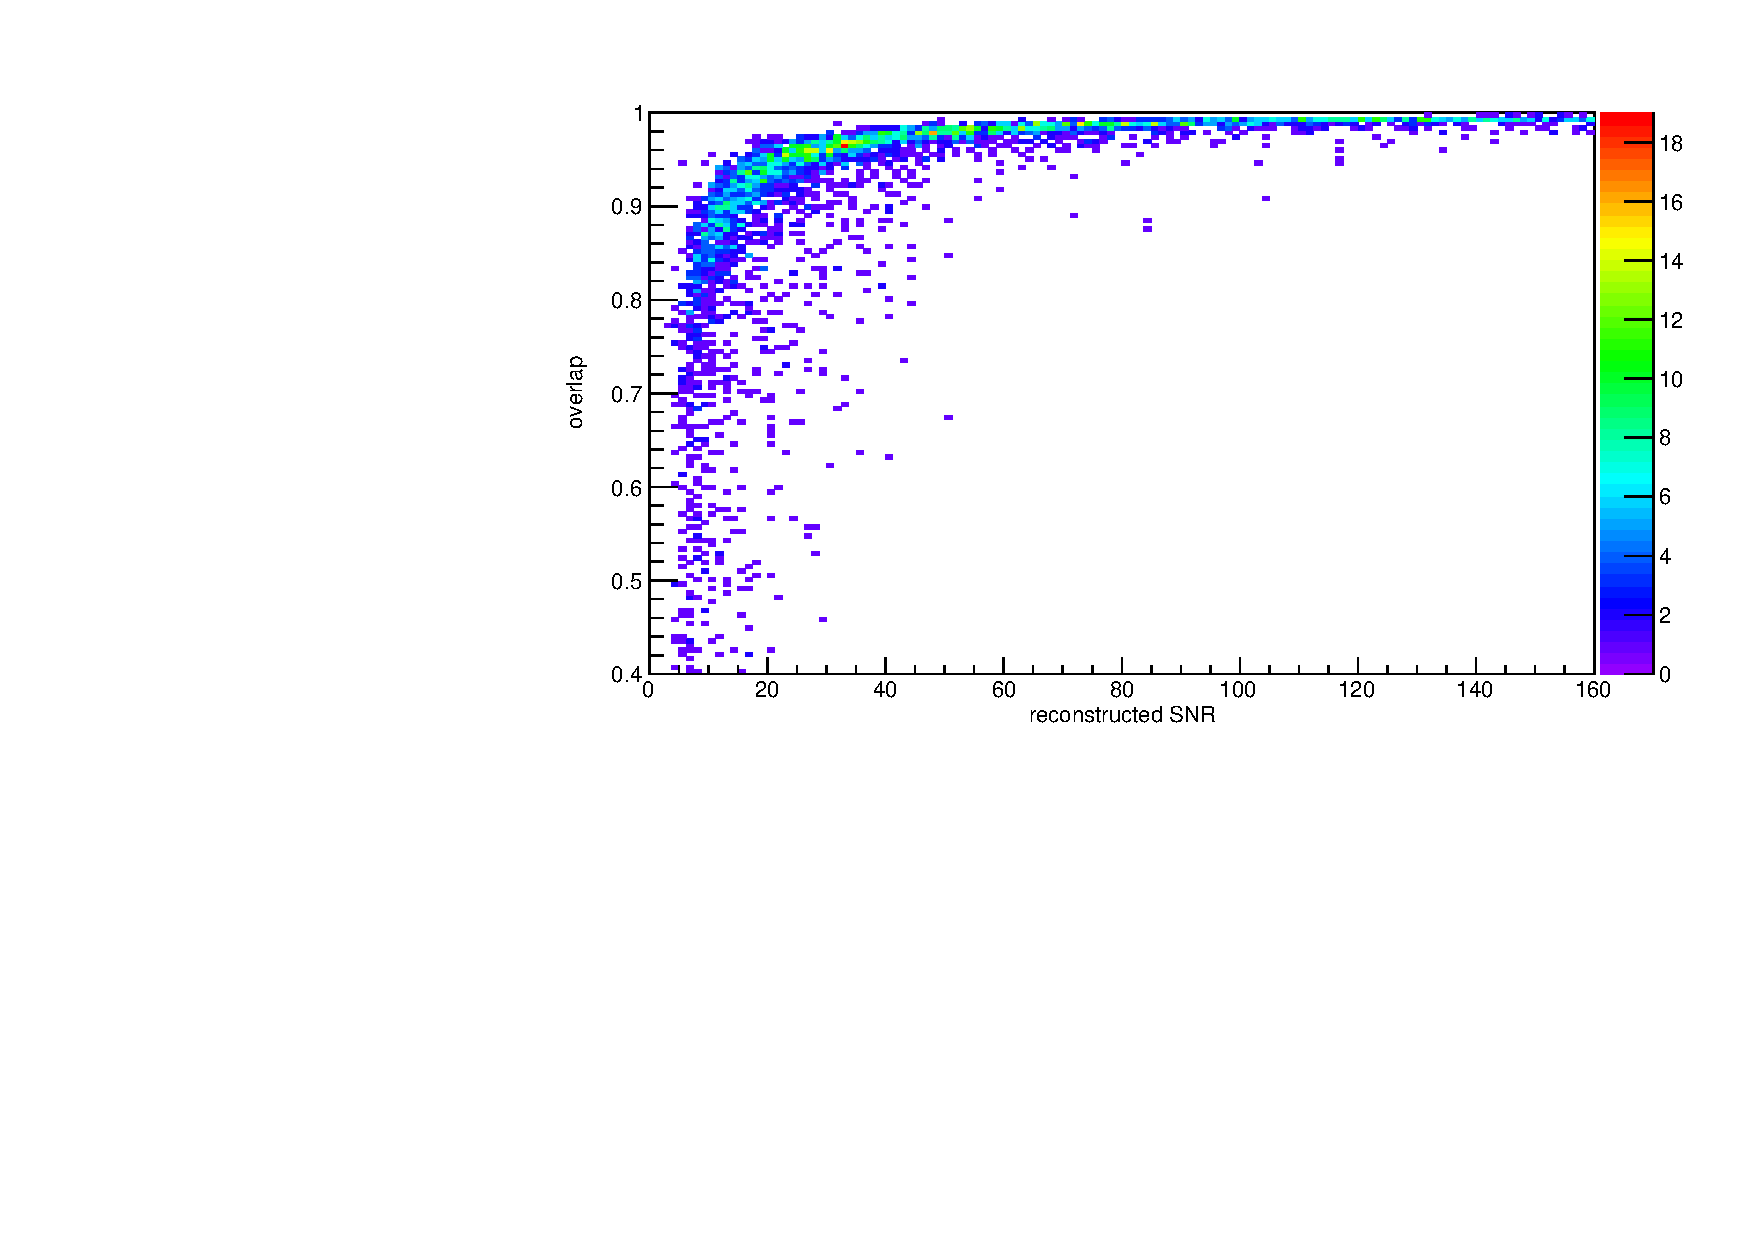
\includegraphics[width=.33\textwidth]{figures/Capitolo_4/report/OverlapDistributionDetector2SHT2_2spin1.pdf}}
	\subfloat[][\emph{SHT2.2 per Virgo}]
	{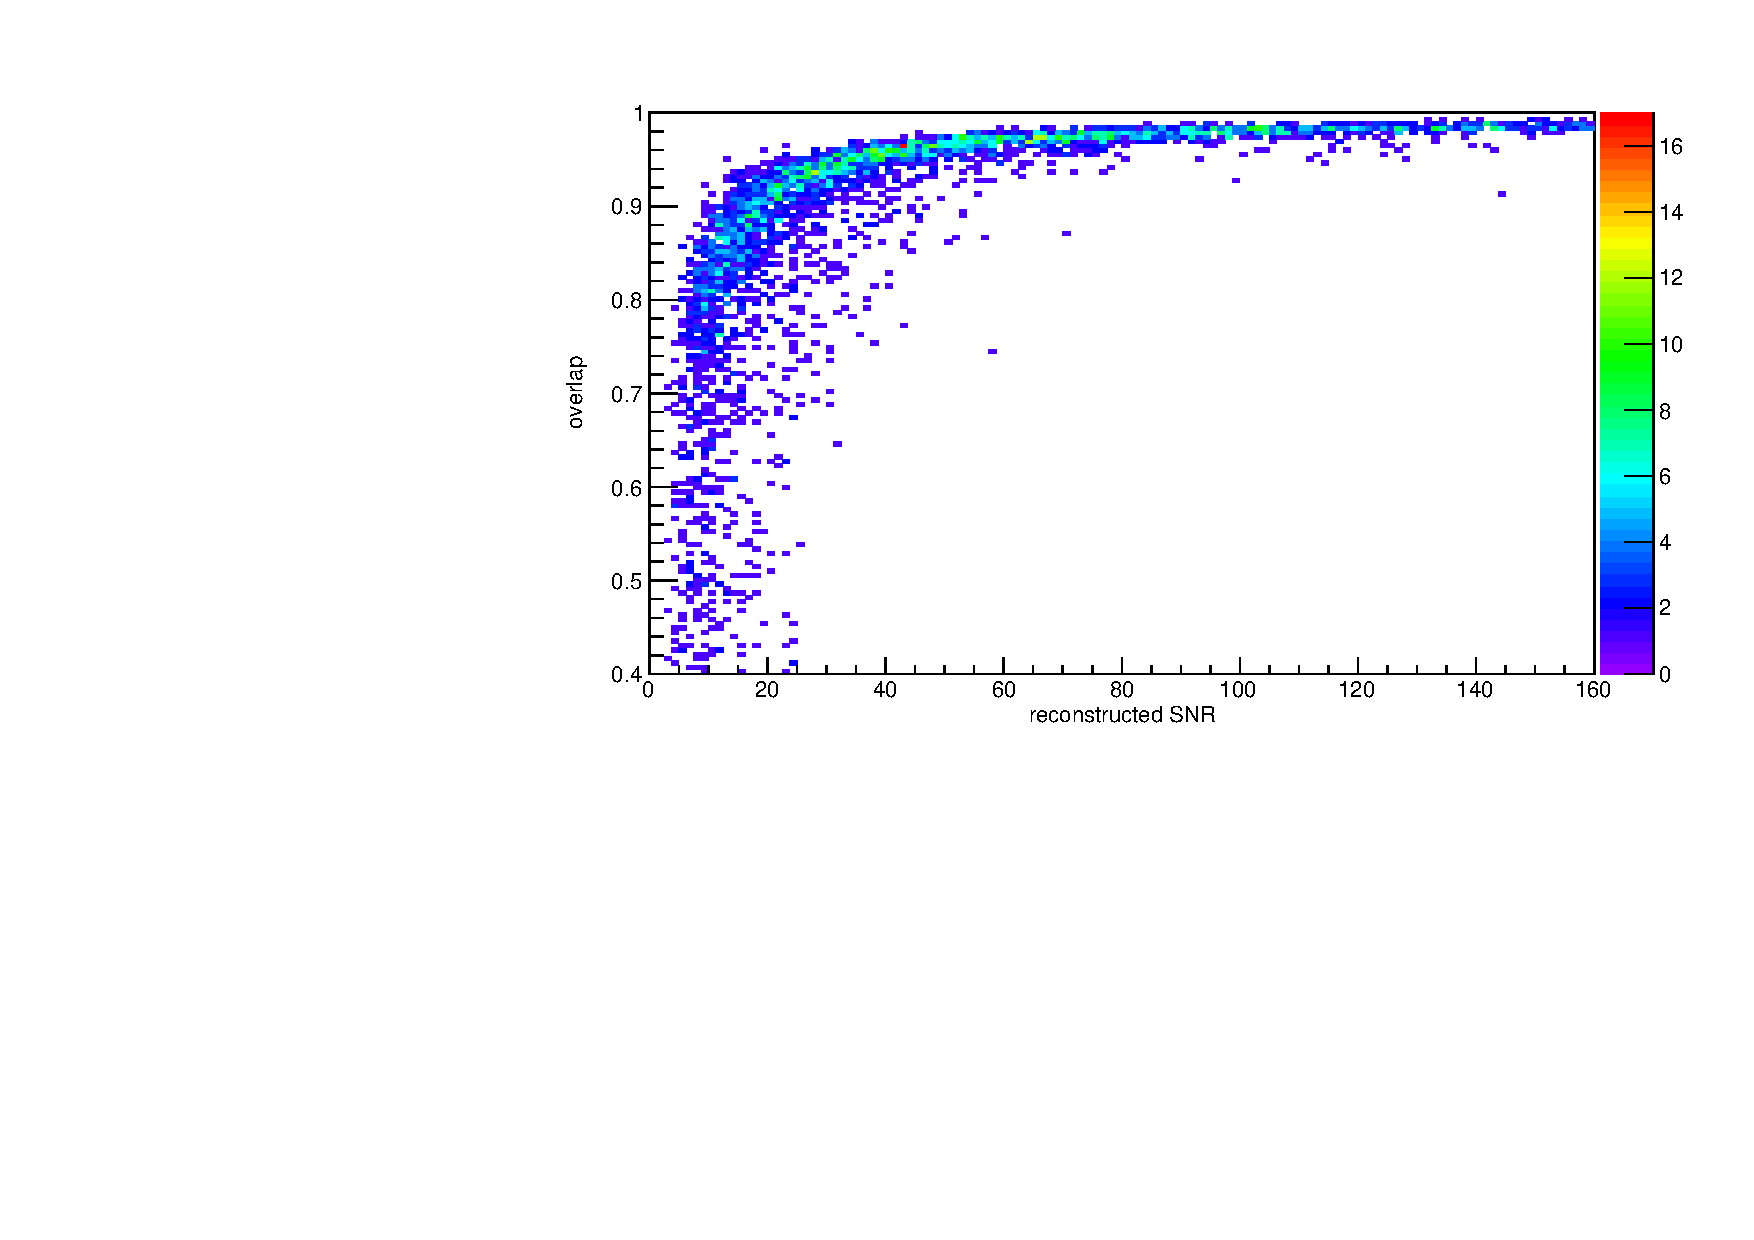
\includegraphics[width=.33\textwidth]{figures/Capitolo_4/report/OverlapDistributionDetector3SHT2_2spin1.pdf}}
	\vspace{-13pt}
	\subfloat[][\emph{APR4 per LIGO-Hanford}]
	{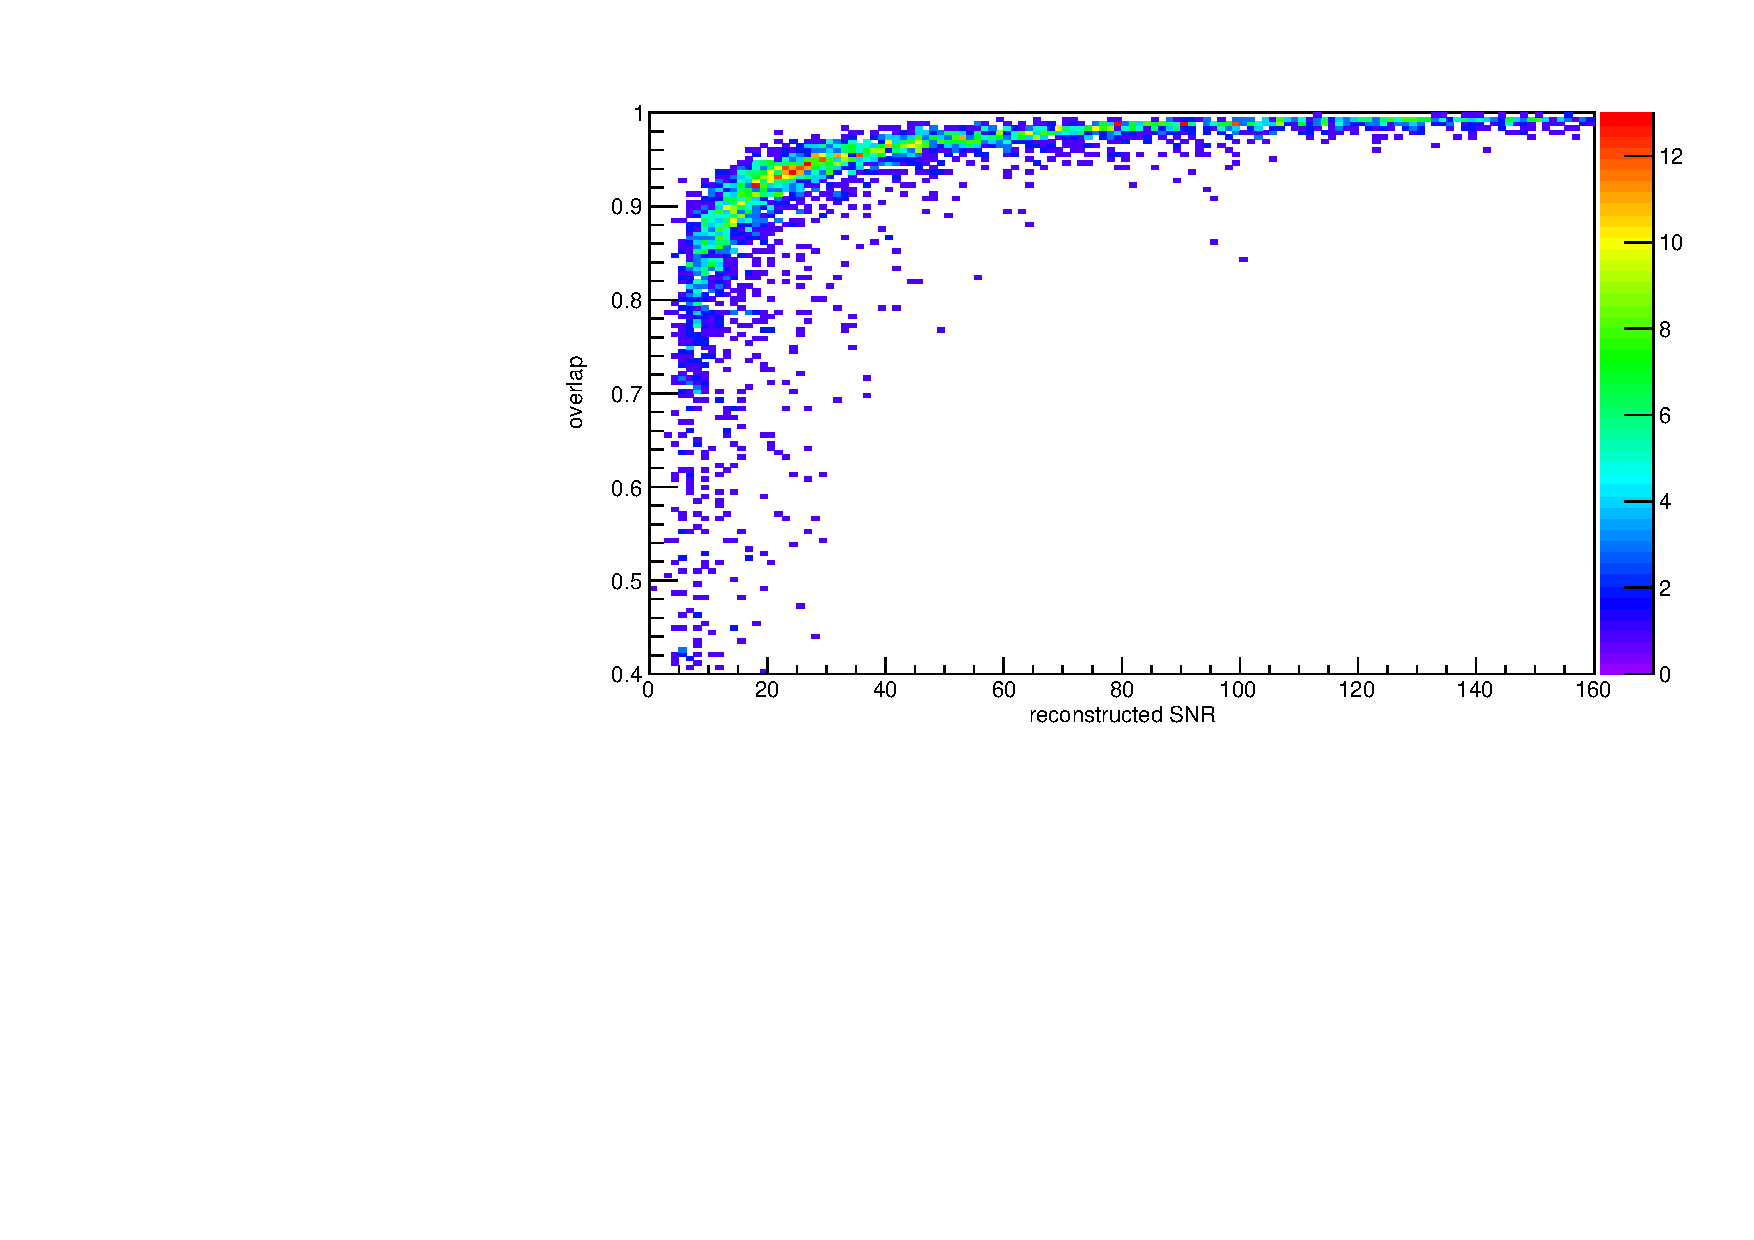
\includegraphics[width=.33\textwidth]{figures/Capitolo_4/report/OverlapDistributionDetector1APR4_q09.pdf}}
	\subfloat[][\emph{APR4 per LIGO-Livingston}]
	{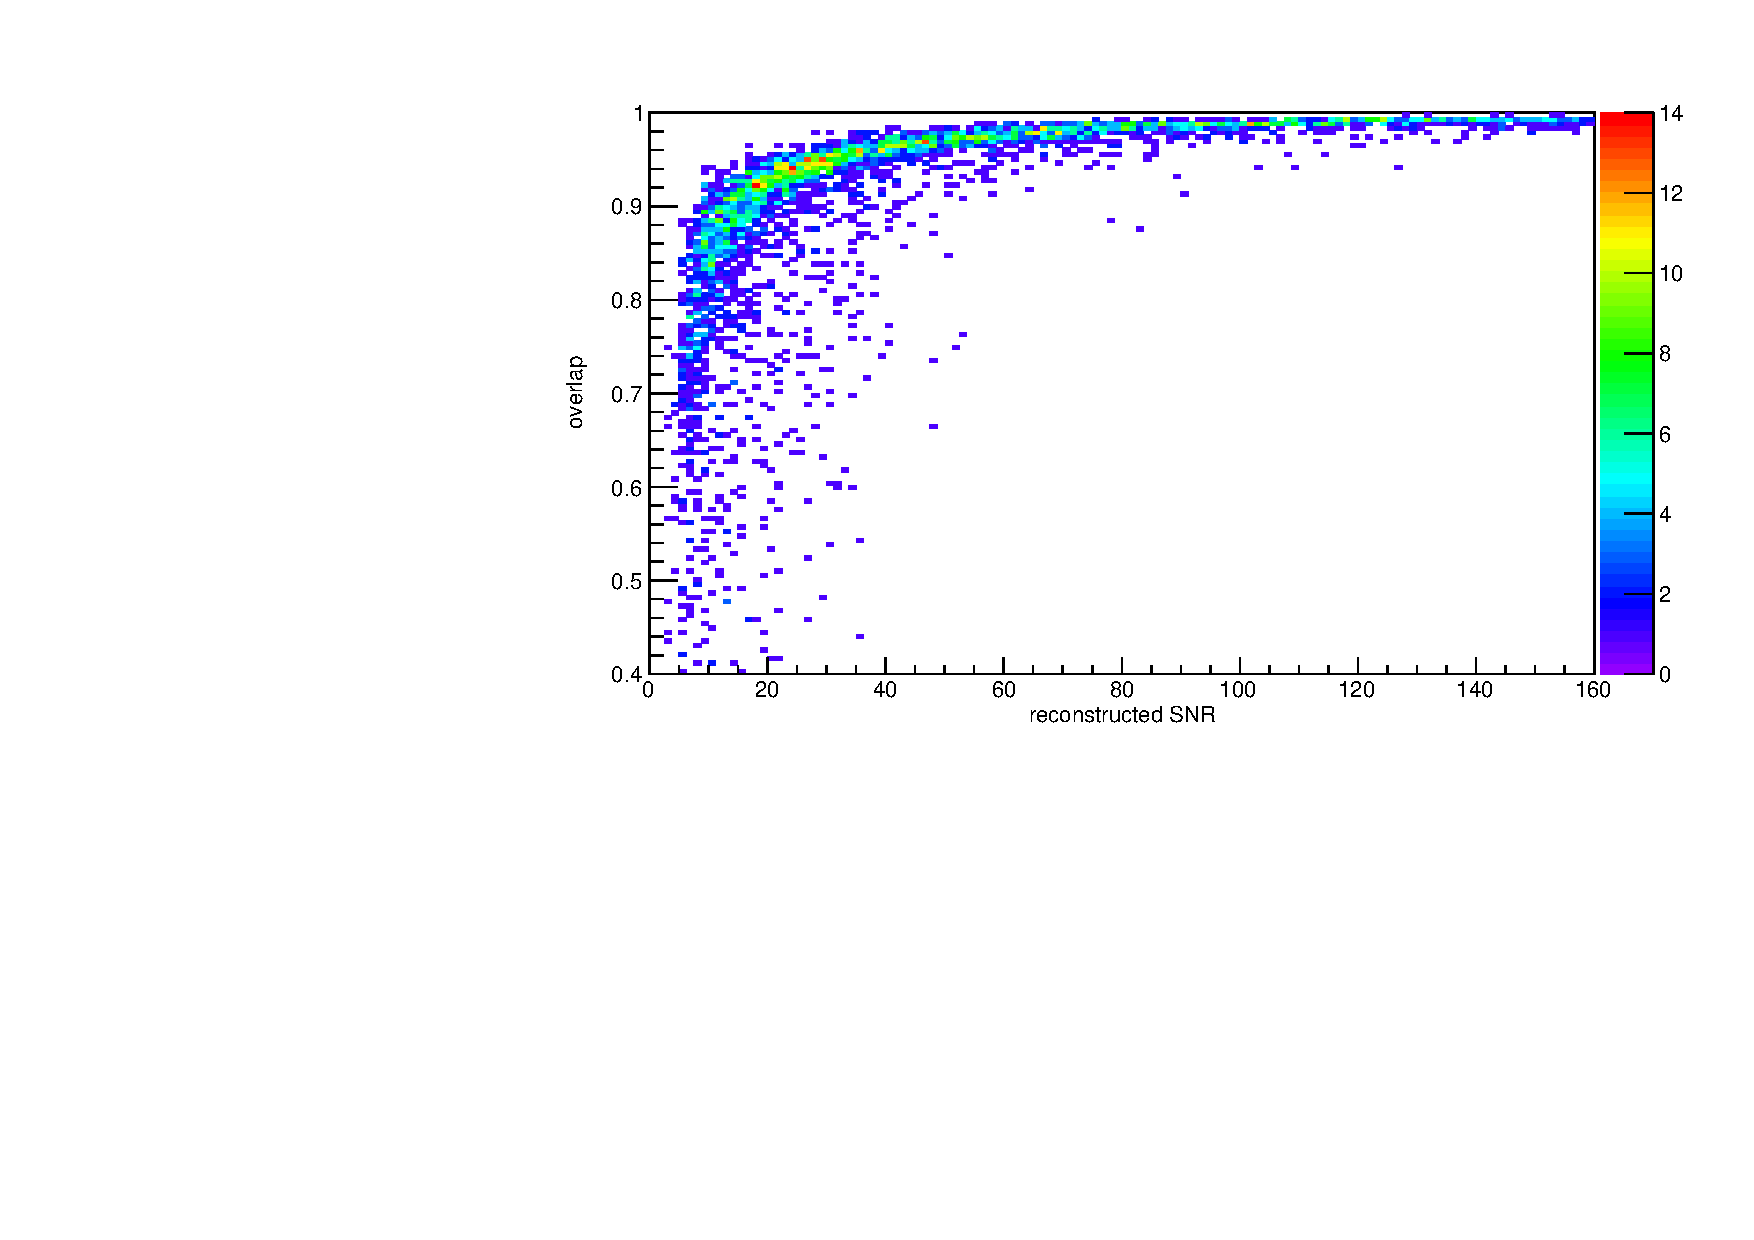
\includegraphics[width=.33\textwidth]{figures/Capitolo_4/report/OverlapDistributionDetector2APR4_q09.pdf}}
	\subfloat[][\emph{APR4 per Virgo}]
	{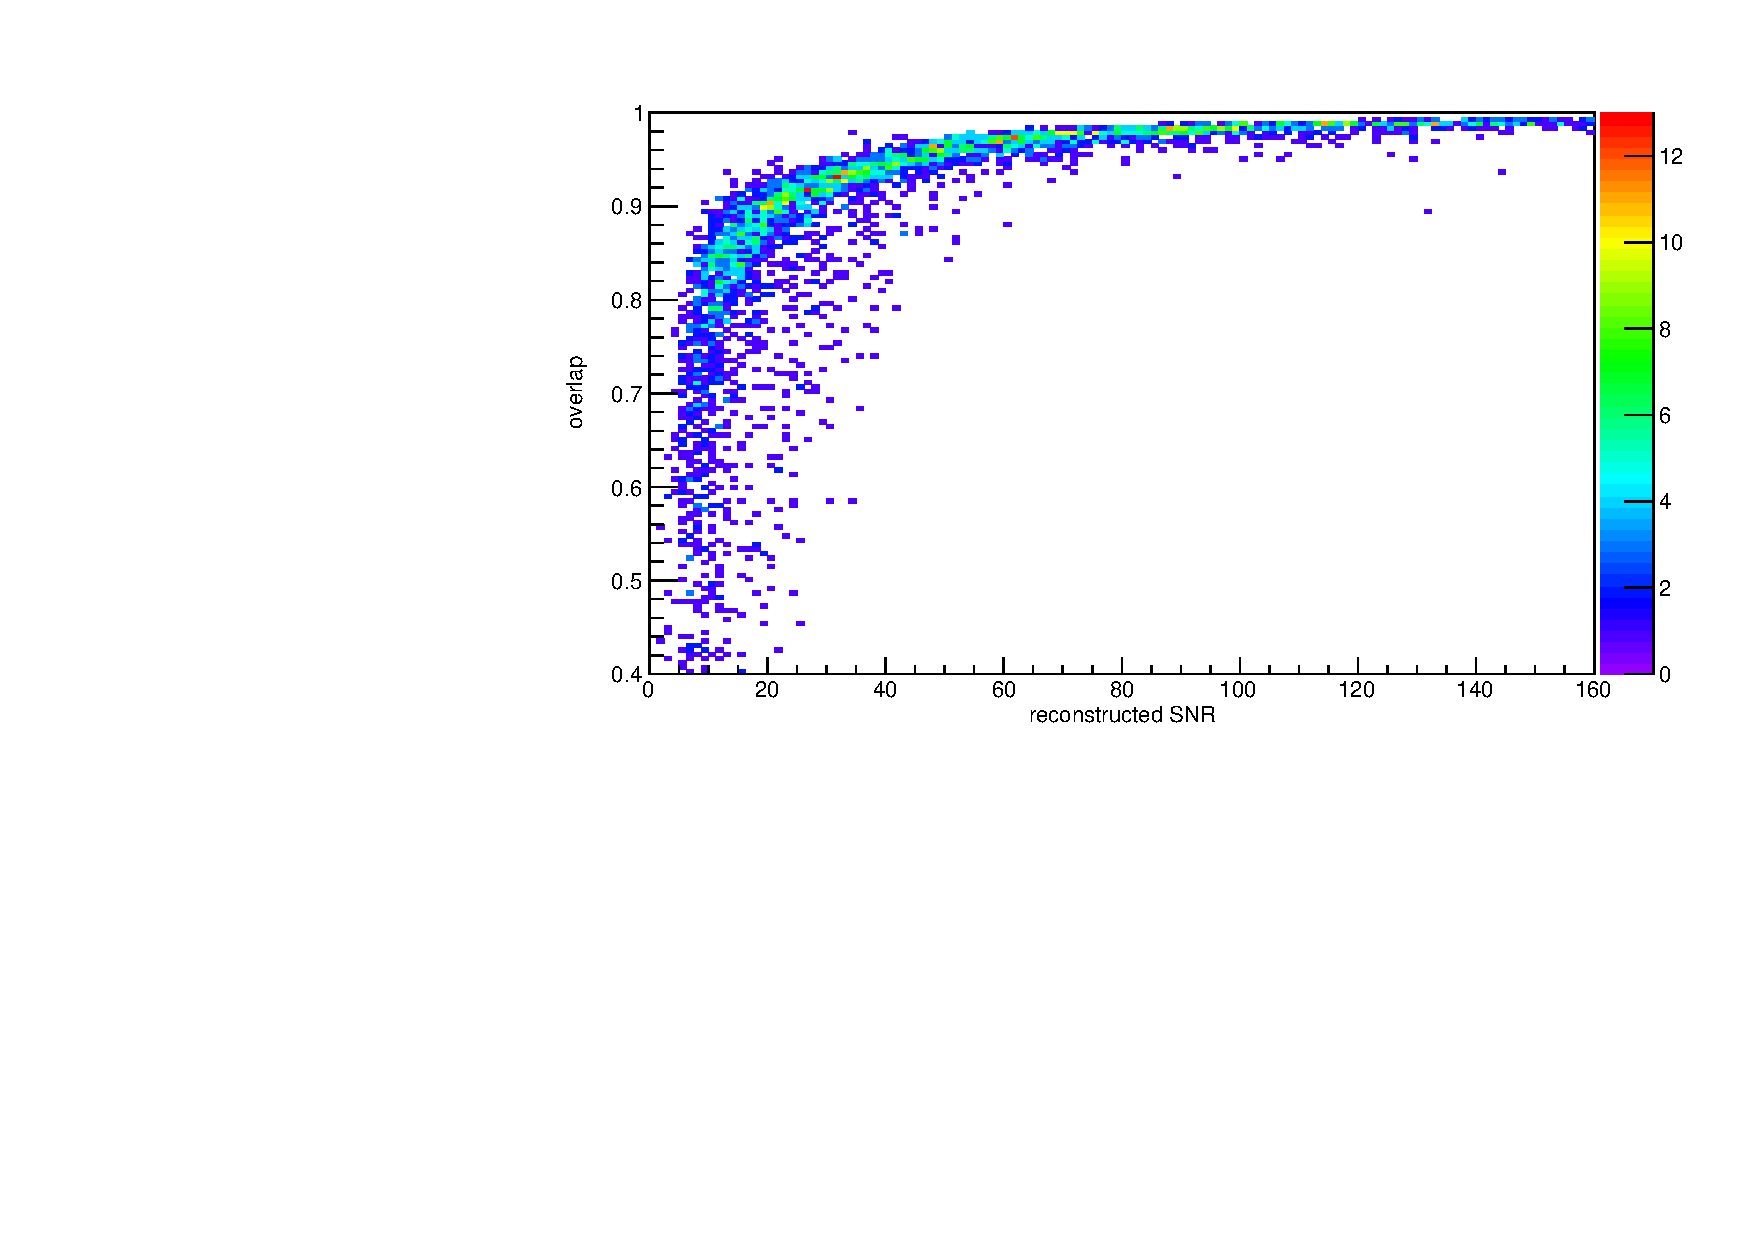
\includegraphics[width=.33\textwidth]{figures/Capitolo_4/report/OverlapDistributionDetector3APR4_q09.pdf}}
	\vspace{-5pt}
	\caption{Overlap in funzione dell'energia del rivelatore}
	\label{fig:Overlap_SHT2_APR4}
	\vspace{-15pt}
\end{figure}
%Il problema si ripresenta anche in questi grafici dove è possibile notare come vi sia per la EOS APR4 una certa quantità che non presenta l'andamento atteso. Si sono isolati gli eventi problematici e si è individuata la ragione della discrepanza: gli eventi che sporcano le distribuzioni sono tali perché vengono spezzati in fase di ricostruzione, c'è infatti una soglia in tempo e in frequenza dopo la quale due eccessi di potenza vengono spezzati in due eventi separati e può accadere, in particolare per la EOS APR4 che, come si è visto in \ref{subsection:APR4}, presenta un post merger a frequenze molto alte. Poiché la fase tra i due segnali, a bassa energia, non sempre viene ricostruita può accadere che il segnale venga spezzato in uno più energetico riguardante l'inspiral e uno meno, legato al post-merger. Questo si nota in particolar modo andando a confrontare la distribuzione delle frequenze minime e massime per le due EOS:
%\begin{figure}[H]
%	\vspace{-25pt}
%	\centering
%	\subfloat[][\emph{SHT2.0}]
%	{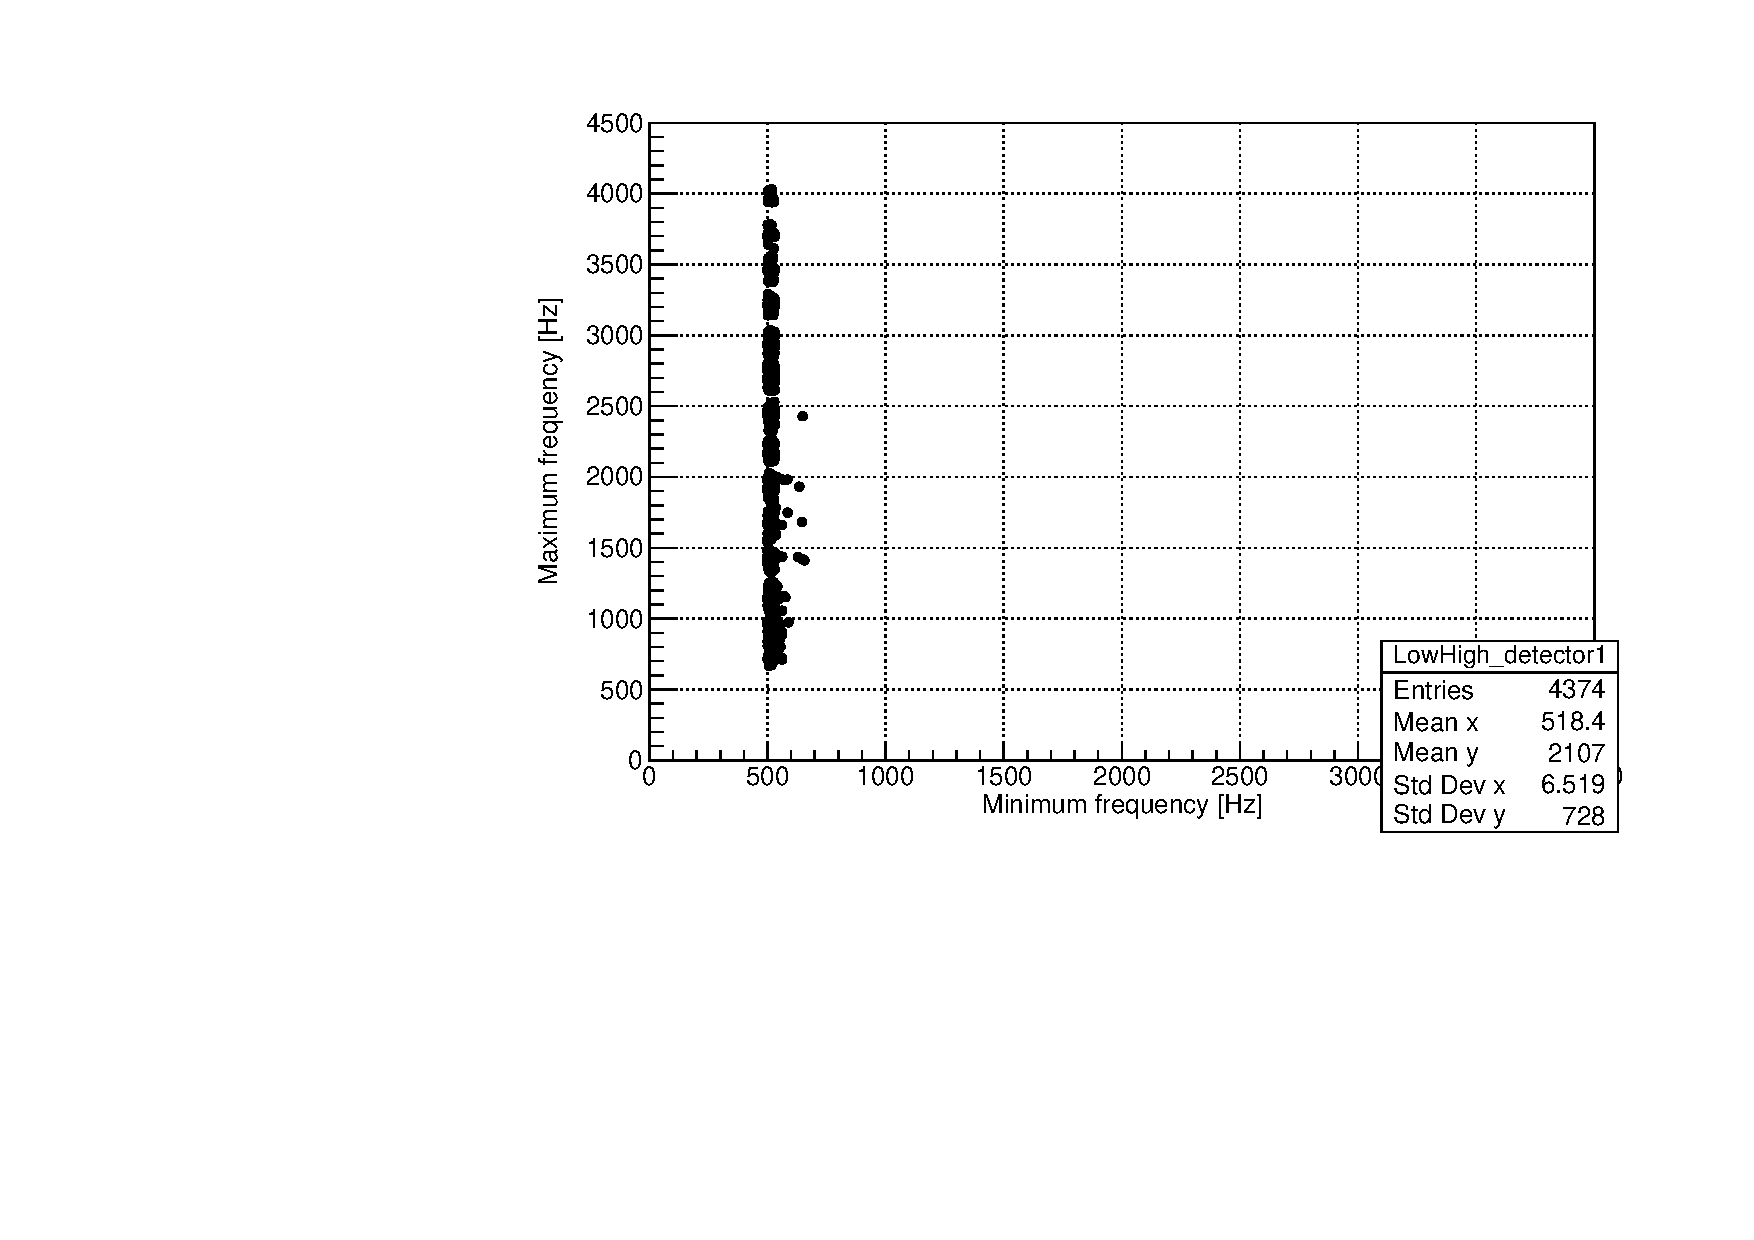
\includegraphics[width=.5\textwidth]{figures/Capitolo_4/FrequencyLHDistributionDetector1SHT2_0spin1.pdf}}% \quad\quad
%	\subfloat[][\emph{APR4}]
%	{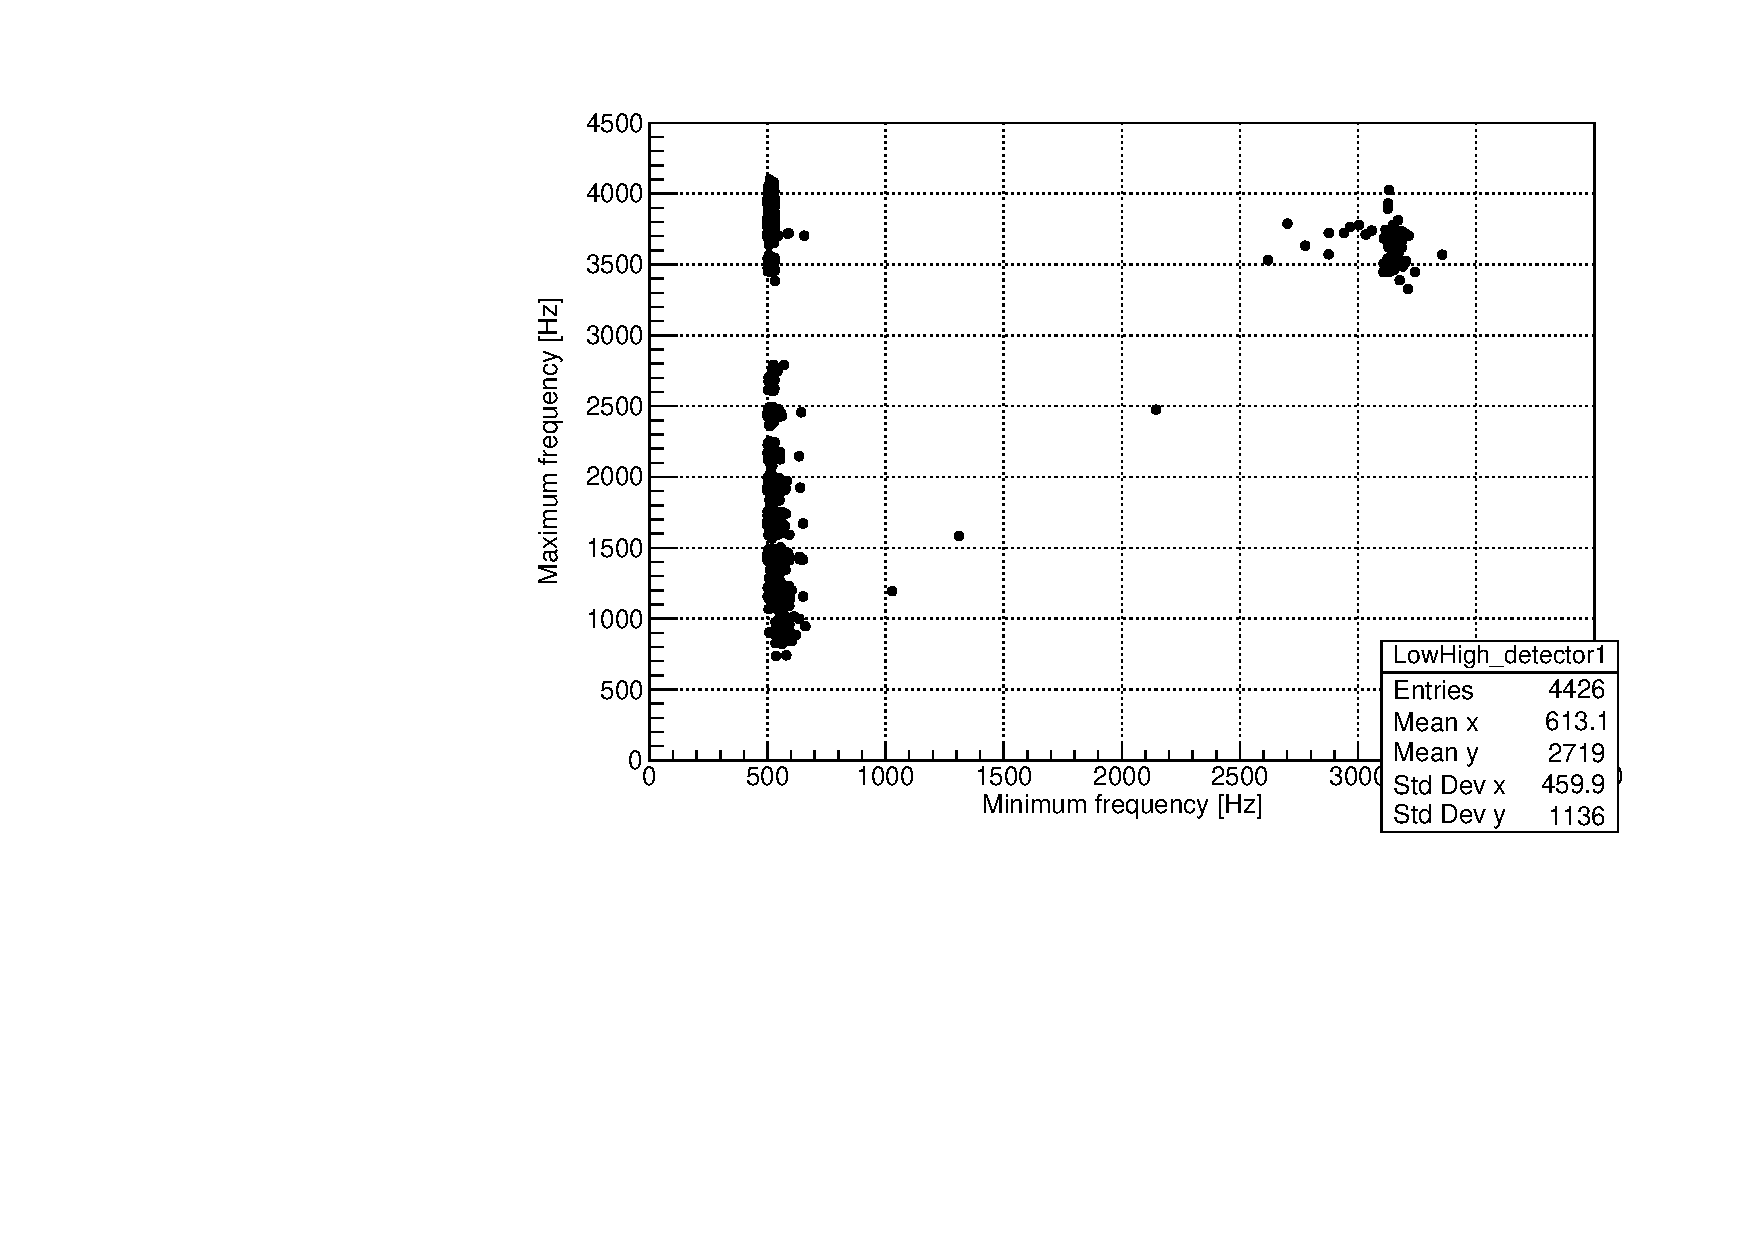
\includegraphics[width=.5\textwidth]{figures/Capitolo_4/FrequencyLHDistributionDetector1APR4_q09.pdf}}
%	\vspace{-5pt}
%	\caption{Distribuzione della frequenza massima e minima per le due EOS}
%	\label{fig:Ffrequency_max_min}
%	\vspace{-15pt}
%\end{figure}
%Si nota immediatamente per la EOS APR4 un cluster di eventi che presenta frequenza minima estremamente alta, incompatibile con l'andamento che assume un evento ricostruito in modo completo, che come descritto in precedenza dovrebbe avere l'andamento di un chirp, partendo da frequenza basse fino a un picco. Vengono quindi tagliati gli eventi ricostruiti nel solo post-merger. 
%Ripetendo le precedenti analisi con il set di ricostruzioni tagliato si ottiene:
%\begin{figure}[H]
%	\vspace{-5pt}
%	\centering
%	\subfloat[][\emph{FIT}]
%	{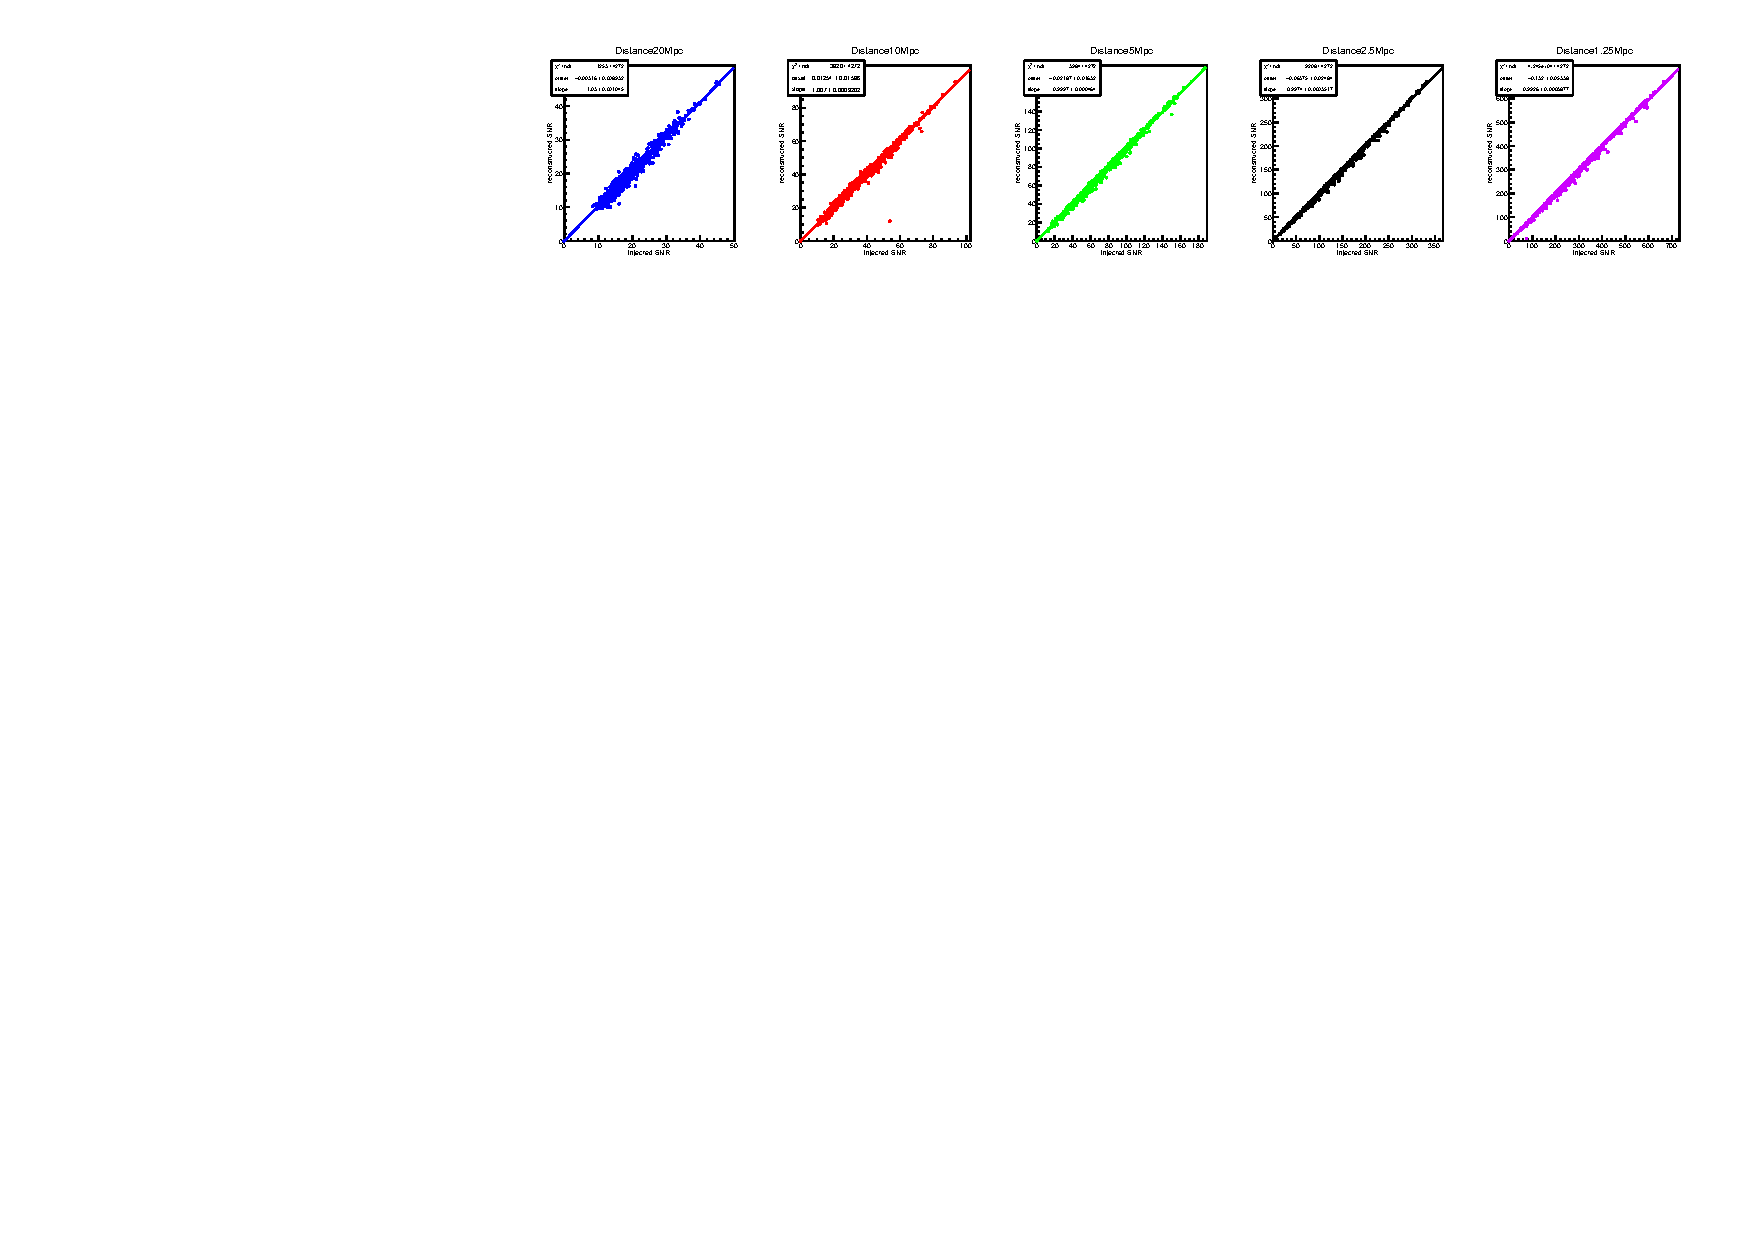
\includegraphics[width=1\textwidth]{figures/Capitolo_4/FITAPR4_q09_CUT.pdf}}\\
%	\vspace{-10pt}
%	\subfloat[][\emph{Energia residua per LIGO-Hanford}]
%	{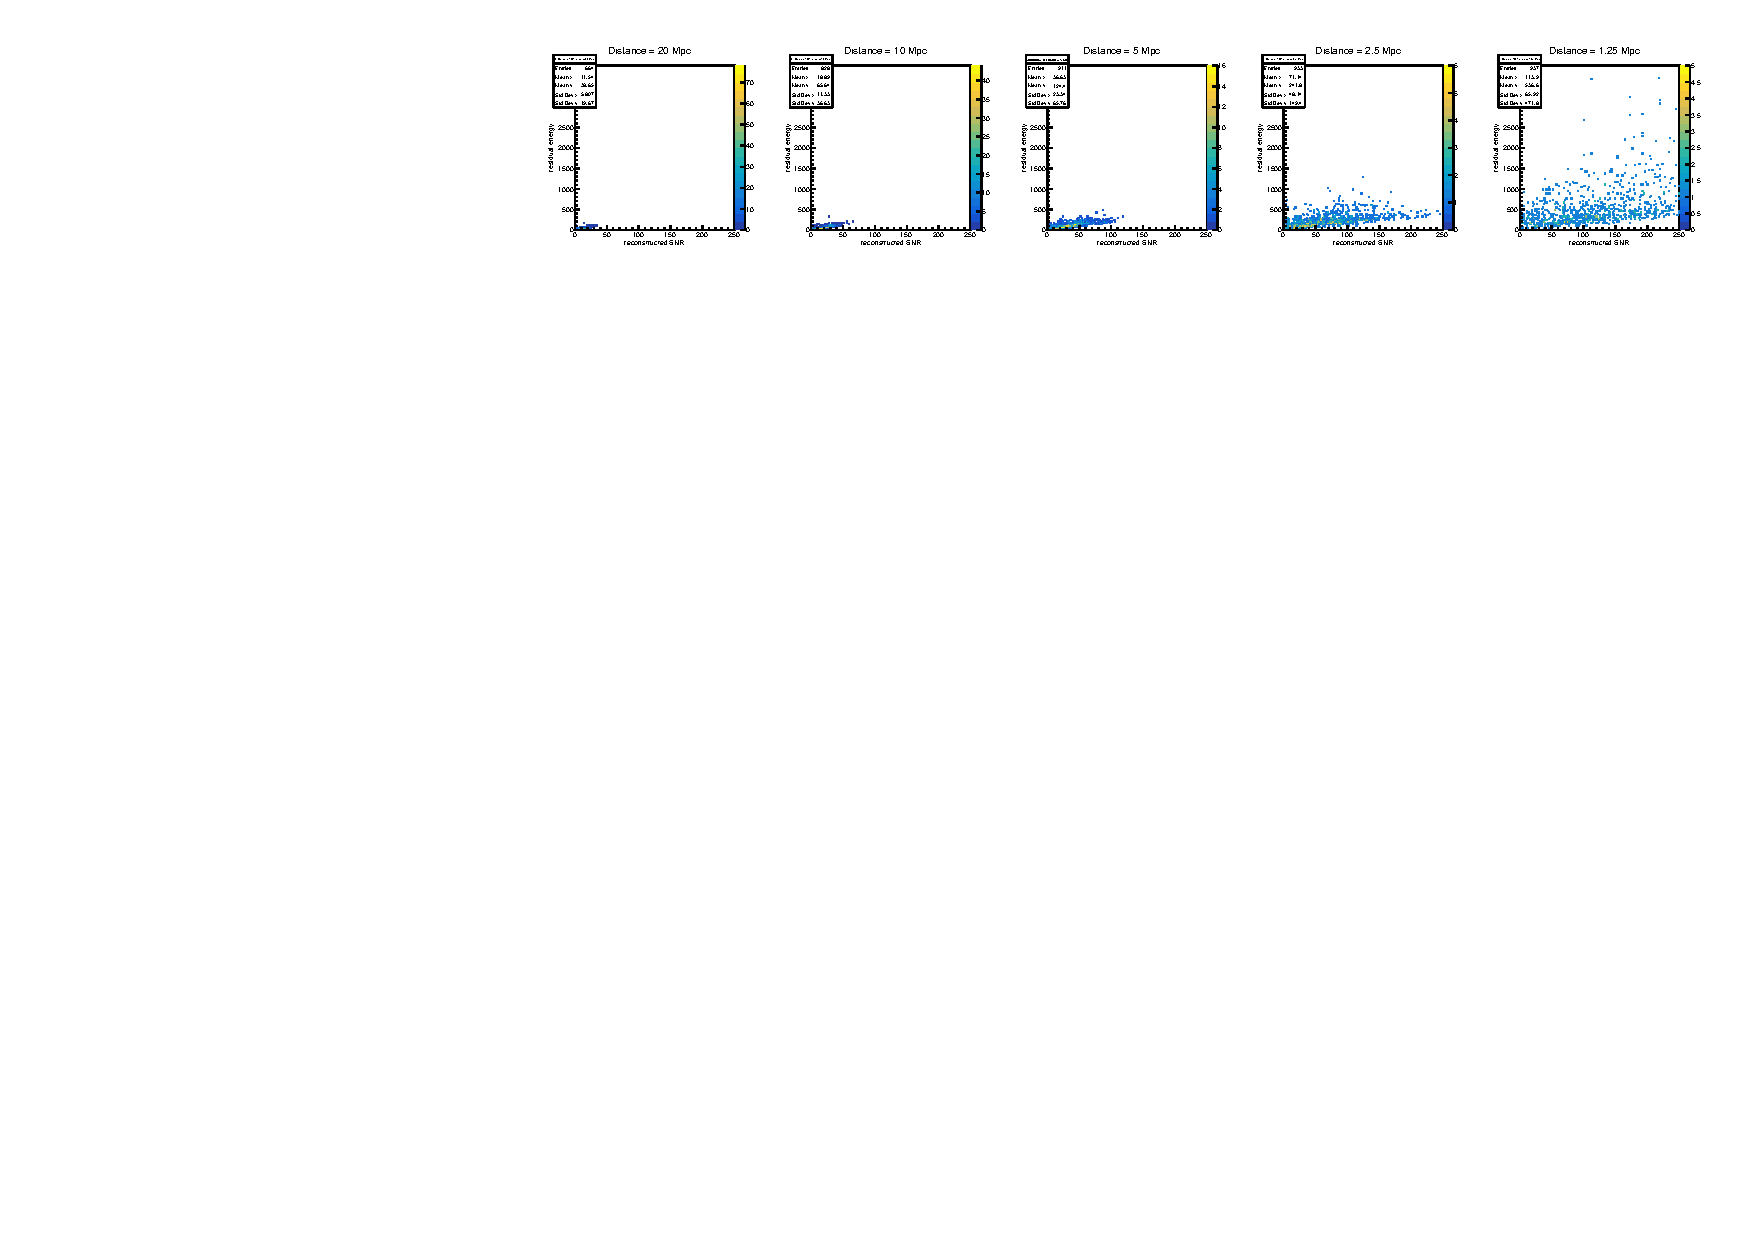
\includegraphics[width=1\textwidth]{figures/Capitolo_4/EnergyDistributionFactorDetector1APR4_q09_CUT.pdf}} \\
%	\vspace{-10pt}
%	\subfloat[][\emph{Overlap per LIGO-Hanford}]
%	{\includegraphics[width=1\textwidth]{figures/Capitolo_4/OverlapDistributionFactorDetector2APR4_q09_CUT.pdf}} 
%	\vspace{-5pt}
%	\caption{Analisi per APR4, fatta escludendo le ricostruzioni separate di uno stesso evento}
%	\label{fig:apr4_cut}
%	\vspace{-15pt}
%\end{figure}
%che presenta risultati non ottimali, come avviene per la EOS SHT2, ma comunque decisamente migliori rispetto ai dati non tagliati.
\begin{wrapfigure}{r}{0.33\textwidth}
	\vspace{-10pt}
	\begin{center}
		\includegraphics[width=.33\textwidth]{figures/Capitolo_4/report/OverlapDistributionsALLDetector1APR4_q09.pdf}
	\end{center}
	\vspace{-12pt}
	\caption{Distribuzioni degli overlap divisi per SNR ricostruito, NON SI CAPISCE}
	\label{fig:overlaps_histo}
	\vspace{-15pt}
\end{wrapfigure}
Gli overlap sono poi stati divisi in bin di SNR ricostruito di larghezza fissata per osservare la distribuzione con la quale i segnali sono ricostruiti, che è riportata in Figura \ref{fig:overlaps_histo}, quindi viene riportato in Figura \ref{fig:Overlap_distribution} l'andamento dei valori medi, con la disperione di ogni bin, rappresentata della deviazione standard.\\
%\begin{figure}[H]
%	\vspace{-15pt}
%	\centering
%	\subfloat[][\emph{SHT2.0}]
%	{\includegraphics[width=.485\textwidth]{figures/Capitolo_4/OverlapDistributionsDetector1SHT2_0spin1.pdf}} \quad
%	\subfloat[][\emph{APR4}]
%	{\includegraphics[width=.485\textwidth]{figures/Capitolo_4/OverlapDistributionsDetector1APR4_q09_CUT.pdf}}
%	\vspace{-5pt}
%	\caption{Distribuzione degli overlap per le due EOS}
%	\label{fig:Distributions_overlap}
%	\vspace{-15pt}
%\end{figure}
%\begin{figure}[H]
%	\vspace{-10pt}
%	\centering
%	\includegraphics[width=1\textwidth]{figures/Capitolo_4/report/OverlapDistributionsDetector1APR4_q09.pdf}
%	\vspace{-15pt}
%	\caption{Distribuzione degli overlap per la EOS APR4 per il solo detector LIGO-Hanford, non si riportano, per ragioni di spazio, i grafici per gli altri detector e per l'altra EOS}
%	\label{fig:Distributions_overlap}
%	\vspace{-15pt}
%\end{figure}
%\begin{figure}[H]
%	\vspace{-15pt}
%	\centering
%	\subfloat[][\emph{SHT2.0}]
%	{\includegraphics[width=.5\textwidth]{figures/Capitolo_4/Overlaps_GrapgDetector1SHT2_0spin1.pdf}}
%	\subfloat[][\emph{APR4}]
%	{\includegraphics[width=.5\textwidth]{figures/Capitolo_4/Overlaps_GrapgDetector1APR4_q09_CUT.pdf}}
%	\vspace{-5pt}
%	\caption{Distribuzione degli overlap per le due EOS}
%	\label{fig:Overlap_distribution}
%	\vspace{-15pt}
%\end{figure}
\begin{figure}[ht]
	\vspace{-10pt}
	\centering
	\subfloat[][\emph{SHT2.0}]
	{\includegraphics[width=.3333333333333333\textwidth]{figures/Capitolo_4/report/overlaps_Colors_GrapgSHT2_0spin1.pdf}}
	\subfloat[][\emph{SHT2.2}]
	{\includegraphics[width=.3333333333333333\textwidth]{figures/Capitolo_4/report/overlaps_Colors_GrapgSHT2_2spin1.pdf}}
	\subfloat[][\emph{APR4}]
	{\includegraphics[width=.3333333333333333\textwidth]{figures/Capitolo_4/report/overlaps_Colors_GrapgAPR4_q09.pdf}}
	\vspace{-5pt}
	\caption{Distribuzione degli overlap per le tre EOS}
	\label{fig:Overlap_distribution}
	\vspace{-15pt}
\end{figure}
Si può notare come le ricostruzioni per Virgo risultino avere una curva di Overlap sistematicamente sottostante a quelle dei due rivelatori LIGO: questo è dovuto alla minore sensibilità di Virgo a frequenze intermedie (Fig.\ref{fig:sensitivity_O4}), dove si manifesta il contributo più energetico che è ottenuto dai rivelatori, per cui la ricostruzione di Virgo, nel contesto di uniformità della posizione celeste e della polarizzazione, sarà necessariamente peggiore.
\paragraph{EOS APR4} Si sottolinea che, in realtà, l'analisi svolta per gli eventi con equazione di stato APR4 ha richiesto un passaggio ulteriore: essendo per questa EOS il segnale di post-coalescenza a frequenze particolarmente elevate si genera un problema nella ricostruzione: i segnali di coalescenza e quelli di post-coalescenza venivano spezzati in due eventi separati, generando incongruenze. L'effetto descritto si può notare nei grafici in Figura \ref{fig:Overlap_problem}, dove si vede un inconsistenza nella curva di overlap (a sinistra) che viene spiegata dagli eventi spezzati: nel grafico delle frequenze massime e minime si vede infatti un bunch di dati che ha frequenza minima estremamente alta, comportamento incompatibile con l'andamento che assume un evento ricostruito in modo completo, che come descritto in precedenza dovrebbe avere l'andamento di un chirp, partendo da frequenza basse fino a un picco.\\
Per ovviare a tale problematica la strategia adottata ha previsto inizialmente il tentativo di allargare la forbice delle frequenze aumentando il valore di soglia da 128Hz fino a 512Hz, con il rischio, però di andare a raccogliere eccessi di rumore e avendo come risultato un segnale non pulito. Il tentativo non ha tuttavia risolto il problema: nella maggioranza dei casi il segnale di coalescenza viene ricostruito a partire da una frequenza più distante di 512Hz rispetto alla fine del segnale di coalescenza, causando una stima peggiore del segnale complessivo senza un significativo miglioramento sul segnale di post-coalescenza. \\
Il problema è invece stato risolto utilizzando un comando di cWB che permette, a partire dalle ricostruzioni, di tagliare, tra gli eventi spezzati, l'evento meno energetico. In questo modo si perde parte degli eventi ricostruiti ma vengono risolte le incongruenze.
\begin{figure}[ht]
	\vspace{-20pt}
	\centering
	\subfloat[][\emph{Overlap}]
	{\includegraphics[width=.4\textwidth]{figures/Capitolo_4/OverlapDistributionDetector1APR4_q09.pdf}}
	\subfloat[][\emph{Frequenza minima e massima}]
	{\includegraphics[width=.4\textwidth]{figures/Capitolo_4/FrequencyLHDistributionDetector1APR4_q09.pdf}}
	\vspace{-5pt}
	\caption{Distribuzione degli overlap e della frequenza massima ricostruita in funzione della minima}
	\label{fig:Overlap_problem}
	\vspace{-10pt}
\end{figure}
\section{Ricerca frequenza post-merger}
\label{section:Frequenza_PM}
%\begin{minipage}{0.65\textwidth}
%	Per valutare la frequenza della post-coalescenza del segnale ricostruito l'analisi, sviluppata in \cite{Puecher_2018} e \cite{Tringali_2017}, segue alcuni step fondamentali. Partendo dalla mappa tempo-frequenza del segnale, questa viene divisa in 4 quadranti, tagliando il piano sia in tempo che in frequenza. In particolare la mappa tempo-frequenza è ottenuta con una trasformazione di wavelet andando a combinare vari layer con diverse larghezze dei bin in frequenza $df$ e in tempo $dt$, definendo l'area dei pixel $df\times dt$ con energia data dall'ampiezza del pixel. Per questa analisi, poiché il segnale si sviluppa su scale temporali estremamente ridotte, per poter distinguere in modo adeguato la parte finale dello spiraleggiamento e della post-coalescenza si utilizza la minima divisione in tempo, corrispondente a 1 ms, che però, essendo l'area del pixel costante porta ad un'estrema imprecisione nella divisione in frequenza pari 512 Hz.\\
%	Il taglio in frequenza è deciso in modo arbitrario in $f = 1792$Hz, comunque al di sotto della soglia di minima 2KHz. In questo modo, facendo un taglio opportuno nell'asse dei tempi, si potrà isolare il segnale di post-coalescenza e la parte finale della coalescenza nel quadrante con $t>t_{cut}$ e $f>f_{cut}$. Per decidere l'istante di tempo in cui produrre il taglio viene fatta una media pesata con l'energia dei pixel per ogni layer.\\
%	Il taglio in frequenza è deciso in modo arbitrario in $f = 1792$Hz, comunque al di sotto della soglia di minima 2KHz. In questo modo, facendo un taglio opportuno nell'asse dei tempi, si potrà isolare il segnale di post-coalescenza e la parte finale della coalescenza nel quadrante con $t>t_{cut}$ e $f>f_{cut}$. Per decidere l'istante di tempo in cui produrre il taglio viene fatta una media pesata con l'energia dei pixel per ogni layer 
%	\begin{equation}
%	\bar{t}_j = \frac{\sum_{i=1}^Nt_{j,i}e_{i,j}}{E_{j}}
%	\end{equation}
%	dove j e i iterano sul layer e sul bin temporale rispettivamente, N è il numero di bin, $t_{j,i}$ e $e_{i,j}$ sono il tempo e l'energia del pixel (j, i) e infine $E_{j} = \sum_{i}e_{j,i}$ è l'energia totale del layer. Il taglio è preso quindi come $t_{cut} = \bar{t}_2 + dt$ con $\bar{t}_2$ tempo stimato per il merger, poiché quest'ultimo ha generalmente frequenze comprese tra 768Hz e 1280Hz corrispondenti al layer 2. Per gli eventi con SNR ricostruito limitato, non avendo segnale nel layer 2, il tempo per il taglio è preso a $t_{cut} = \bar{t}_1 + 5dt$. Si osserva comunque che questo metodo non è ottimale, andando a raccogliere anche parte del late-merger portando a una sottostima sistematica.
%\end{minipage}
%È poi interessante valutare il peso relativo del segnale di post coalescenza al rapporto segnale su rumore, rispetto al segnale complessivo. Per fare questo è utile mostrare l'SNR cumulativo in funzione del tempo: si può notare come il contributo della post-coalescenza risulti estremamente ridotto in rapporto alla fase di spiraleggiamento, a prova dell'estrema difficoltà nel rivelare questa fase del segnale.

%\begin{wrapfigure}{r}{0.4\textwidth}
%	\vspace{-25pt}
%	\begin{center}
%		\includegraphics[width=0.4\textwidth]{figures/Capitolo_4/dump/501/wdm64_501_2_layers64_rec_cut.png}
%	\end{center}
%	\vspace{-5pt}
%	\caption{Mappa tempo frequenza del segnale ricostruito per Virgo per EOS SHT2.0}
%	\label{fig:tfm_intero}
%	\vspace{-5pt}
%\end{wrapfigure}
Per valutare la frequenza della post-coalescenza del segnale ricostruito l'analisi, sviluppata in \cite{Puecher_2018} e \cite{Tringali_2017}, segue alcuni step fondamentali: partendo dalla mappa tempo-frequenza del segnale, questa viene divisa in 4 quadranti, tagliando il piano sia in tempo che in frequenza. In particolare la mappa tempo-frequenza è ottenuta con una trasformazione di wavelet andando a combinare vari layer con diverse larghezze dei bin in frequenza $df$ e in tempo $dt$, definendo l'area dei pixel $df\times dt$ con energia data dall'ampiezza del pixel. Per questa analisi, poiché il segnale si sviluppa su scale temporali estremamente ridotte, per poter distinguere in modo adeguato la parte finale dello spiraleggiamento e della post-coalescenza si utilizza la minima divisione in tempo, corrispondente a 1 ms, che però, essendo l'area del pixel costante porta ad un'estrema imprecisione nella divisione in frequenza pari 512 Hz.

\begin{figure}[ht]
	\vspace{-20pt}
	\centering
	\subfloat[][\emph{Segnale completo}]
	{\includegraphics[width=.4\textwidth]{figures/Capitolo_4/dump/501/wdm64_501_2_layers64_rec_cut.png}}\quad\quad
	\subfloat[][\emph{Segnale post-coalescenza}]
	{\includegraphics[width=.4\textwidth]{figures/Capitolo_4/dump/501/wdm64_501_2_layers64_recPM2.png}}
	\vspace{-8pt}
	\caption{Distribuzione delle energie della post coalescenza in funzione dell'energia totale ricostruita in Virgo}
	\label{fig:time_freq_pm}
	\vspace{-8pt}
\end{figure}
%\begin{wrapfigure}{r}{0.46\textwidth}
%	\vspace{-35pt}
%	\begin{center}
%		\includegraphics[width=0.46\textwidth]{figures/Capitolo_4/dump/476/V1_476.png}
%	\end{center}
%	\vspace{-5pt}
%	\caption{Forma d'onda ricostruita per Virgo per EOS SHT2.0}
%	\label{fig:segnale_tempo}
%	\vspace{-10pt}
%\end{wrapfigure}
%\begin{wrapfigure}{r}{0.4\textwidth}
%	\vspace{-45pt}
%	\begin{center}
%		\includegraphics[width=0.4\textwidth]{figures/Capitolo_4/dump/501/wdm64_501_2_layers64_recPM2.png}
%	\end{center}
%	\vspace{-5pt}
%	\caption{Rappresentazione tempo-frequenza del segnale per Virgo per EOS SHT2.0, terzo quadrante}
%	\label{fig:3quadrante}
%	\vspace{-25pt}
%\end{wrapfigure}
Il taglio in frequenza è deciso in modo arbitrario in $f = 1792$Hz, comunque al di sotto della soglia di minima 2KHz. In questo modo, facendo un taglio opportuno nell'asse dei tempi, si potrà isolare il segnale di post-coalescenza e la parte finale della coalescenza nel quadrante con $t>t_{cut}$ e $f>f_{cut}$. \\ 
\begin{wrapfigure}{r}{0.4\textwidth}
	\vspace{-30pt}
	\begin{center}
		\includegraphics[width=0.4\textwidth]{figures/Capitolo_4/dump/501/V1_snr_cum_SHTdfdt_501.png}
	\end{center}
	\vspace{-8pt}
	\caption{SNR cumulativo}
	\label{fig:snr_cum}
	\vspace{-10pt}
\end{wrapfigure}
Per decidere l'istante di tempo in cui produrre il taglio viene fatta una media pesata con l'energia dei pixel per ogni layer
\begin{equation}
	\bar{t}_j = \frac{\sum_{i=1}^Nt_{j,i}e_{i,j}}{E_{j}}
\end{equation}
dove j e i iterano sul layer e sul bin temporale rispettivamente, N è il numero di bin, $t_{j,i}$ e $e_{i,j}$ sono il tempo e l'energia del pixel (j, i) e infine $E_{j} = \sum_{i}e_{j,i}$ è l'energia totale del layer. Il taglio è preso quindi come $t_{cut} = \bar{t}_2 + dt$ con $\bar{t}_2$ tempo stimato per il merger, poiché quest'ultimo ha generalmente frequenze comprese tra 768Hz e 1280Hz corrispondenti al layer 2. Per gli eventi con SNR ricostruito limitato, non avendo segnale nel layer 2, il tempo per il taglio è preso a $t_{cut} = \bar{t}_1 + 5dt$. Si osserva comunque che questo metodo non è ottimale, andando a raccogliere anche parte della fine dello spiraleggiamento portando a una sottostima sistematica della frequenza.

È poi interessante valutare il peso relativo del segnale di post coalescenza all'energia ricostruita, rispetto al segnale complessivo. Per fare questo è utile mostrare l'SNR cumulativo in funzione del tempo, in Figura \ref{fig:snr_cum}, si può notare come il contributo della post-coalescenza risulti estremamente ridotto in rapporto alla fase di spiraleggiamento, a prova dell'estrema difficoltà nel rivelare questa fase del segnale.

Questo procedimento è stato fatto, come per l'analisi precedente, sistematicamente su un grande numero di eventi ricostruiti in modo da poterne valutare l'efficienza e studiare i risultati. Si riporta in Figura \ref{fig:energy_pm_colz} l'energia stimata per il segnale di post-coalescenza, in funzione dell'energia totale per le diverse distanze: è facile intuire che per gli eventi a distanza maggiore il segnale di post-coalescenza viene rivelato in casi molto limitati, avvicinandosi il segnale diventa invece sempre più energetico. \\
Si osserva inoltre che per la EOS SHT2.2, in cui non è atteso alcun segnale di post-coalescenza, poiché come si osserva in Figura \ref{fig:forme_onda} il sistema ha un ringdown e non c'è emissione di segnali dopo la coaelescenza, si registra energia significativa anche nella post-coalescenza. Questo risulta quindi un importante limite del metodo utilizzato: non permette di distinguere segnali con e senza post-coalescenza. Si osserva comunque che gli eventi ricostruiti sono meno numerosi e meno energetici.
\begin{figure}[ht]
	\vspace{-10pt}
	\centering
	\subfloat[][\emph{SHT2\_0}]
	{\includegraphics[width=1.\textwidth]{figures/Capitolo_4/report/EnergyDistributionFactorDetector3SHT2_0spin1.pdf}}\\
	\vspace{-13pt}
	\subfloat[][\emph{SHT2\_2}]
	{\includegraphics[width=1.\textwidth]{figures/Capitolo_4/report/EnergyDistributionFactorDetector3SHT2_2spin1.pdf}}\\
	\vspace{-13pt}
	\subfloat[][\emph{APR4}]
	{\includegraphics[width=1.\textwidth]{figures/Capitolo_4/report/EnergyDistributionFactorDetector3APR4_q09.pdf}}
	\caption{Distribuzione delle energie della post coalescenza in funzione dell'energia totale ricostruita in Virgo}
	\label{fig:energy_pm_colz}
\end{figure}\\
Con una costruzione analoga a quella fatta per l'overlap, quindi con la divisione degli eventi in bin di SNR, si costruisce la distribuzione delle energie della post-coalescenza, riportata in Figura \ref{fig:energy_pm_Distrib}. Si nota che il segnale ricostruito da Virgo è sistematicamente più energetico del segnale ricostruito da LIGO, grazie alla maggior sensibilità del primo ad alte frequenza. Si sottilinea che comunque la sensibilità di Virgo è sovrastimata per l'assenza della caratterizzazione di risonanze e altri fenomeni che ne comprometterebbero la sensibilità.
\begin{figure}[ht]
	\vspace{-15pt}
	\centering
	\subfloat[][\emph{SHT2\_0}]
	{\includegraphics[width=.33333333333\textwidth]{figures/Capitolo_4/report/energy_pm_Colors_GrapgSHT2_0spin1.pdf}}
	\subfloat[][\emph{SHT2\_2}]
	{\includegraphics[width=.33333333333\textwidth]{figures/Capitolo_4/report/energy_pm_Colors_GrapgSHT2_2spin1.pdf}}
	\subfloat[][\emph{APR4}]
	{\includegraphics[width=.33333333333\textwidth]{figures/Capitolo_4/report/energy_pm_Colors_GrapgAPR4_q09.pdf}}
	\caption{Distribuzione delle energie della post coalescenza in funzione dell'energia totale ricostruita nei tre rivelatori}
	\label{fig:energy_pm_Distrib}
\end{figure}

Si valuta poi la frequenza alla quale vengono ricostruiti i segnali di post-coalescenza, in Figura \ref{fig:frequency_pm_colz}, e le distribuzioni divendo per bin di SNR a larghezza fissata, in Figura \ref{fig:frequency_pm_Distrib}. Quello che si osserva è che la frequenza ricostruita risulta generalmente superiore per Virgo, rispetto ai rivelatori LIGO, per motivi analoghi a quello che porta segnali più energetici per il primo. È interessante anche osservare l'andamento che non è strettamente crescente in funzione dell'energia ricostruita, ma parte da frequenze più alte e dopo un minimo risale: questa peculiarità è spiegata dalla distribuzione dell'energia nella post-coalesenza, che risulta avere un picco corrispondente anche al picco di frequenza. Essendo quindi il picco più energetico, sarà la parte che verrà ricostruita prima, e quindi eventi meno energetici, in cui si ricostruisce la post-coalescenza, faranno riferimento al solo picco. Superata questa fase, la ricostruzione avviene come atteso.\\
Si osserva inoltre, come atteso, che le frequenze ricostruite, essendo frequenze pesate, risultano sottostimate poiché nella ricostruzione viene considerata la parte finale dello spiraleggiamento, a frequenze evidentemente inferiori.
%\begin{figure}[ht]
%	\vspace{-15pt}
%	\centering
%	\subfloat[][\emph{SHT2\_0}]
%	{\includegraphics[width=1.\textwidth]{figures/Capitolo_4/report/Freq_PM_DistributionFactorDetector1SHT2_0spin1.pdf}}\\
%	\vspace{-13pt}
%	\subfloat[][\emph{SHT2\_2}]
%	{\includegraphics[width=1.\textwidth]{figures/Capitolo_4/report/Freq_PM_DistributionFactorDetector1SHT2_2spin1.pdf}}\\
%	\vspace{-13pt}
%	\subfloat[][\emph{APR4}]
%	{\includegraphics[width=1.\textwidth]{figures/Capitolo_4/report/Freq_PM_DistributionFactorDetector1APR4_q09.pdf}}
%	\caption{Distribuzione delle energie della post coalescenza in funzione dell'energia totale ricostruita in Virgo}
%	\label{fig:frequency_pm_colz}
%\end{figure}
\begin{figure}[ht]
	\vspace{-15pt}
	\centering
	\subfloat[][\emph{SHT2\_0}]
	{\includegraphics[width=.333333333333333333\textwidth]{figures/Capitolo_4/report/Freq_PM_DistributionDetector3SHT2_0spin1.pdf}}
	\subfloat[][\emph{SHT2\_2}]
	{\includegraphics[width=.333333333333333333\textwidth]{figures/Capitolo_4/report/Freq_PM_DistributionDetector3SHT2_2spin1.pdf}}
	\subfloat[][\emph{APR4}]
	{\includegraphics[width=.333333333333333333\textwidth]{figures/Capitolo_4/report/Freq_PM_DistributionDetector3APR4_q09.pdf}}
	\caption{Distribuzione delle energie della post coalescenza in funzione dell'energia totale ricostruita in Virgo}
	\label{fig:frequency_pm_colz}
\end{figure}
\begin{figure}[ht]
	\vspace{-15pt}
	\centering
	\subfloat[][\emph{SHT2\_0}]
	{\includegraphics[width=.33333333333\textwidth]{figures/Capitolo_4/report/frequencies_Colors_GrapgSHT2_0spin1.pdf}}
	\subfloat[][\emph{SHT2\_2}]
	{\includegraphics[width=.33333333333\textwidth]{figures/Capitolo_4/report/frequencies_Colors_GrapgSHT2_2spin1.pdf}}
	\subfloat[][\emph{APR4}]
	{\includegraphics[width=.33333333333\textwidth]{figures/Capitolo_4/report/frequencies_Colors_GrapgAPR4_q09.pdf}}
	\caption{Distribuzione delle frequenze della post coalescenza in funzione dell'energia totale ricostruita nei tre rivelatori}
	\label{fig:frequency_pm_Distrib}
\end{figure}

Si riporta poi, in Figura \ref{fig:bandwidth_pm_Distrib}, la distribuzione della larghezza di banda dei segnali ricostruiti, ovvero la differenza tra la frequenza massima e minima rivelate. Si nota che essa ha un andamento analogo a quello della frequenza, motivo per il quale la probabilità di rivelare il segnale aumenta con l'aumentare dell'SNR.
\begin{figure}[ht]
	%	\vspace{-15pt}
	\centering
	\subfloat[][\emph{SHT2\_0}]
	{\includegraphics[width=.33333333333\textwidth]{figures/Capitolo_4/report/bandwidth_Colors_GrapgSHT2_0spin1.pdf}}
	\subfloat[][\emph{SHT2\_2}]
	{\includegraphics[width=.33333333333\textwidth]{figures/Capitolo_4/report/bandwidth_Colors_GrapgSHT2_2spin1.pdf}}
	\subfloat[][\emph{APR4}]
	{\includegraphics[width=.33333333333\textwidth]{figures/Capitolo_4/report/bandwidth_Colors_GrapgAPR4_q09.pdf}}\\
	\caption{Distribuzione delle larghezze di banda della post coalescenza in funzione dell'energia totale ricostruita nei tre rivelatori}
	\label{fig:bandwidth_pm_Distrib}
\end{figure}

%\begin{figure}[ht]
%	\vspace{-15pt}
%	\centering
%	\subfloat[][\emph{SHT2\_0}]
%	{\includegraphics[width=.33333333333\textwidth]{figures/Capitolo_4/report/hfsnr_Colors_GrapgSHT2_0spin1.pdf}}
%	\subfloat[][\emph{SHT2\_2}]
%	{\includegraphics[width=.33333333333\textwidth]{figures/Capitolo_4/report/hfsnr_Colors_GrapgSHT2_2spin1.pdf}}
%	\subfloat[][\emph{APR4}]
%	{\includegraphics[width=.33333333333\textwidth]{figures/Capitolo_4/report/hfsnr_Colors_GrapgAPR4_q09.pdf}}
%	\caption{Distribuzione delle energie della post coalescenza in funzione dell'energia totale ricostruita nei tre detector}
%	\label{fig:snrhf_Distrib}
%\end{figure}
È interessante anche osservare la distribuzione delle energie della post-coalescenza in funzione della verosimiglianza dell'evento, in Figura \ref{fig:likelihood}.
\begin{figure}[ht]
	\vspace{-15pt}
	\centering
	\subfloat[][\emph{SHT2\_0}]
	{\includegraphics[width=.33333333333\textwidth]{figures/Capitolo_4/report/Likelihood_DistributionDetector1SHT2_0spin1.pdf}}
	\subfloat[][\emph{SHT2\_2}]
	{\includegraphics[width=.33333333333\textwidth]{figures/Capitolo_4/report/Likelihood_DistributionDetector1SHT2_2spin1.pdf}}
	\subfloat[][\emph{APR4}]
	{\includegraphics[width=.33333333333\textwidth]{figures/Capitolo_4/report/Likelihood_DistributionDetector1APR4_q09.pdf}}\\
	\caption{Distribuzione delle energie della post coalescenza in funzione della verosimiglianza dell'evento, per LIGO Livingstone}
	\label{fig:likelihood}
\end{figure}
\section*{Conclusioni}
La rivelazione del primo segnale di onda gravitazionale da un sistema binario di stelle di neutroni nell'Agosto 2017 ha aperto un nuovo ramo di studio della fisica, in particolare per le equazioni di stato delle stelle di neutroni. Dopo la coalescenza, la natura del corpo celeste rimanente è determinata in modo primario dalle masse delle stelle progenitrici e dall'equazione di stato della materia nucleare e questo determina il segnale di post-coalescenza. Purtroppo, a causa della limitata sensibilità dei rivelatori, questa fase del segnale non è stata ancora identificata, nè nel primo segnale rivelato, nè in quello successivo, non permettendo di determinare quale, tra i diversi modelli proposti per le NS, sia quello corretto.

Questa tesi si propone di valutare la capacità di ricostruzione prevista per il run O4, andando a simulare un grande numero di eventi con posizione e polarizzazione casuali e calcolando alcune grandezze che permettono di esprimere quantitativamente l'efficienza dell'algoritmo. In particolare le curve di overlap e di energia residua permettono di fare la caratterizzazione.
La seconda parte dell'analisi si è invece concentrata sulla caratterizzazione del segnale di post-coalescenza che, con il procedimento descritto, viene isolato permettendo di valutarne il contributo in energia, la frequenza pesata e la larghezza di banda pesata. I risultati mostrano che il metodo utilizzato porta a una sottostima sistematica della frequenza, poiché nella media viene considerato anche il contributo della parte finale dello spiraleggiamento, a frequenze significativamente inferiori rispetto alla post-coalescenza. Inoltre il metodo utilizzato non permette di distinguere in modo automatico una coalescenza con stelle progenitrici tali da portare a un buco nero o a stelle di neutroni stabili o instabili. Sarà necessario quindi implementare delle statistiche che permettano di discernere il tipo di segnale che si sta valutando.